

\PassOptionsToPackage{table}{xcolor} % to use colors in tables
\PassOptionsToPackage{pdfa}{hyperref}
\documentclass{unipd-thesis-modern} % src: https://github.com/baronefr/unipd-
\raggedbottom

% additional packages
\usepackage[spanish]{babel}      % Idioma español (separación silábica, etc.)
\usepackage{lipsum} % for DEMO only
\usepackage{threeparttable}
\usepackage{threeparttable}
\usepackage{siunitx}
\usepackage[titles]{tocloft} % to modify spacing in toc chapters
\usepackage{tabularx}
\usepackage{booktabs}
\usepackage{caption}
\usepackage{array}
\usepackage[utf8]{inputenc}
\usepackage{titlesec} % Paquete para controlar espaciado de títulos
\usepackage{graphicx}
\usepackage{float} % para usar [H] si quieres fijar la figura
\usepackage{enumitem}
\usepackage{longtable}
\usepackage{placeins}
\usepackage{adjustbox}
\setlength{\emergencystretch}{3em} % evita Overfull hbox en párrafos con URL y \texttt
%\usepackage{natbib}              % Referencias bibliográficas (comandos \citep, \citet)
\usepackage{tikz}                % Diagramas vectoriales (arquitectura medallón, etc.)
\usetikzlibrary{shapes.geometric, arrows.meta, positioning, calc, babel}
%   IMPORTANTE: la librería 'babel' es OBLIGATORIA cuando se usa babel en español;
%   evita el conflicto entre el carácter '>' activo de babel y la sintaxis '>=stealth' de TikZ.
%
%\usepackage[backend=biber, style=apa]{biblatex}
%   NO cargar natbib junto con biblatex — son incompatibles.
\setlength{\cftbeforechapskip}{7pt}
\setcounter{tocdepth}{4} % ToC depth

% titles
\title{Estimación Municipal Sobre la Tasa de Desempleo en el Cauca y Valle del Cauca: Estimación de Área Pequeña usando Modelos Mixtos y Componentes Espaciales}
\thesisHeader{Pontificia Universidad Javeriana Cali \\Facultad de Ingeniería y Ciencias\\MAESTRÍA EN CIENCIA DE DATOS}
\academicYear{Santiago de Cali, Colombia, 2026}

% student
\author{Samuel Steven Bermúdez Pedraza \\Juan Pablo Rengifo Valencia \\ Felipe Sampedro Giraldo 
}

% supervisor
\advisor{Sandra Milena Ramírez Buelvas}{Pontificia Universidad Javeriana Cali}

% co-advisor (comentar si no hay)
\coadvisor{Iván Gutiérrez}{Universidad Andrés Bello, Chile}


% (optional, comment to remove)
%\otheradvisor{Prof. Paolino Paperino}{University of Padua} % (optional, comment to remove)
% ^ NOTE: you can use optional arg to customize the label "Internal Supervisor"
%   example:   \otheradvisor[The best supervisor!]{Prof. Paolino Paperino}{University of Padua}

% dedication (comment to remove)
\dedication{\textit{A nuestras familias y amigos\\ Samuel, Juan Pablo y Felipe }}

% custom symbols (optional)
%!TEX root = ./main.tex

% Comandos propios del documento.

% Lista de anexos (estructura oficial de la maestría, versión 2025). Cada sección del
% apéndice se abre con \anexo{Título}, que crea la sección y la registra en la lista.
\newlistof{anexos}{loa}{Lista de anexos}
\setlength{\cftanexosnumwidth}{2.8em}
\newcommand{\anexo}[1]{%
  \section{#1}%
  \addcontentsline{loa}{anexos}{\protect\numberline{\thesection}#1}%
}


% bibliography file
\addbibresource{refs.bib}

\sisetup{
  output-decimal-marker = {.},
  group-separator = {,},
  detect-all = true
}


% Ajustes de espacio
\titlespacing*{\subsection}{0pt}{10pt plus 2pt minus 2pt}{5pt}
\titlespacing*{\subsubsection}{0pt}{5pt plus 2pt minus 2pt}{3pt}
% Otros paquetes y configuraciones
\setlength{\intextsep}{6pt}      % Espacio entre texto y figuras
\setlength{\textfloatsep}{6pt}   % Espacio entre texto y flotantes


\begin{document}
\renewcommand{\tablename}{Tabla}
\renewcommand{\listfigurename}{Lista de figuras}
\renewcommand{\listtablename}{Lista de tablas}
    \frontmatter
    % --------------------------
    \chapter*{Introducción}
\addcontentsline{toc}{chapter}{Introducción}

Las encuestas de hogares miden lo que ningún registro administrativo cubre por completo, como la condición de actividad de la población, pero no cubren todo el territorio. Cada dominio para el que se quiere publicar una cifra precisa exige un número mínimo de hogares encuestados, y ese número cuesta en encuestadores, desplazamientos y supervisión. Por eso las encuestas concentran la muestra en los territorios de mayor peso. En Colombia, la Gran Encuesta Integrada de Hogares (GEIH), que realiza el Departamento Administrativo Nacional de Estadística (DANE), es la fuente oficial del mercado laboral, y en 2018 publicaba la tasa de desempleo de 23 ciudades capitales y áreas metropolitanas (A.M.), además de los totales nacional, por zona y por departamento \cite[p.~9]{DANE_GEIH_Metodologia2016}.

El resultado es que no se conoce la tasa de desempleo de los municipios medianos y pequeños. En el Cauca y el Valle del Cauca, 81 de los 84 municipios no tienen ninguna estimación directa, y los tres que la tienen se miden dentro de una ciudad o un área metropolitana. Las políticas de empleo de esos municipios se diseñan con la cifra del departamento o de la capital, aunque la evidencia para Colombia muestra que el desempleo municipal difiere mucho de un lugar a otro y que esas diferencias persisten \cite[pp.~124--125]{Diaz2016}.

La estimación en áreas pequeñas (SAE, por sus siglas en inglés) se desarrolló para este tipo de vacío: combina la encuesta con información auxiliar disponible para todo el territorio y, con un modelo ajustado a los dominios que sí tienen muestra, estima el indicador en los que no la tienen \cite[p.~17]{Molina2019}. Este trabajo usó el modelo de Fay-Herriot \cite{FayHerriot1979}, que tiene dos partes. El modelo de muestreo trata la tasa directa de la GEIH de cada dominio como una medición con error de su valor verdadero, con una varianza conocida. El modelo de enlace relaciona ese valor verdadero con covariables municipales de TerriData, el sistema de estadísticas territoriales del Departamento Nacional de Planeación (DNP), más un efecto aleatorio de área. Se probó además una extensión espacial, en la que los efectos de áreas cercanas pueden estar correlacionados.

La metodología se organizó en 16 etapas. Se integraron la GEIH de 2018, TerriData, la división político-administrativa del DANE y las cifras publicadas por el DANE; se estimó la tasa de desempleo anual de 23 dominios (ciudades o ciudades con su área metropolitana) con su varianza por bootstrap de viviendas; se seleccionaron covariables de un catálogo construido con la literatura mediante un Fay-Herriot univariado y un control de falsos descubrimientos; se eligió un modelo Fay-Herriot clásico como referencia y se comparó con ocho especificaciones espaciales en condiciones controladas; se validó la estimación de cada dominio retirándolo del ajuste; y se estimó la tasa de 83 municipios del Cauca y del Valle del Cauca, con su error, su estado de extrapolación y un ajuste para que las estimaciones agregadas reprodujeran las cifras directas.

Las tasas directas de los 23 dominios reprodujeron las del DANE y todas resultaron confiables, con coeficientes de variación entre 2.01~\% y 3.23~\%. De 18 covariables candidatas, solo la tasa de homicidios quedó en el modelo, con una asociación positiva que depende de un dominio, Quibdó; al repetir la selección sin cada dominio, el procedimiento estimó peor que un modelo sin covariables. No se encontró evidencia de dependencia espacial: ninguna especificación espacial tuvo una prueba de razón de verosimilitudes significativa y las estimaciones de los dominios coincidieron con las del modelo clásico. Ninguno de los 83 municipios quedó con una estimación confiable, 21 de ellos son extrapolación del modelo, y el patrón territorial de las estimaciones reproduce el de la tasa de homicidios. El aporte del trabajo es, por tanto, la metodología: un procedimiento reproducible que informa con qué calidad y bajo qué supuestos se puede estimar el desempleo de un municipio sin encuesta, y que puede repetirse con mejores covariables.

El documento se organiza así. La Sección~\ref{sec:problema} plantea y formula el problema y la Sección~\ref{sec:objetivos} presenta los objetivos. La Sección~\ref{sec:marco-referencia} reúne el marco teórico y los antecedentes. La Sección~\ref{sec:datos} describe las fuentes de información y la Sección~\ref{sec:metodologia}, las 16 etapas de la metodología. La Sección~\ref{sec:resultados} presenta los resultados de cada etapa en el mismo orden. La Sección~\ref{sec:discusion} discute su alcance y el trabajo futuro, y la Sección~\ref{sec:conclusion} cierra con las conclusiones por objetivo.

    \newpage
    % --------------------------
    \mainmatter
    % --------------------------
    \chapter{Definición del problema}
        \label{sec:problema}

\section{Planteamiento del problema}
\label{sec:planteamiento}

La tasa de desempleo de un municipio colombiano mediano o pequeño no se conoce. La fuente oficial del mercado laboral, la GEIH, es una encuesta por muestreo probabilístico, estratificado y de conglomerados, y su diseño fija de antemano los territorios para los que publica resultados: mensualmente, el conjunto de las 13 grandes ciudades con sus áreas metropolitanas, las 11 ciudades intermedias y el total nacional; trimestral y semestralmente, cada ciudad capital con su área metropolitana, las grandes regiones y las zonas de cabecera y resto; y anualmente, además, cada departamento \cite[p.~9]{DANE_GEIH_Metodologia2016}. El municipio no es un dominio de la encuesta. La muestra se asigna para alcanzar una precisión fijada en esos dominios, un error estándar relativo no mayor al 5~\% para una tasa de desempleo del 10~\% \cite[p.~12]{DANE_GEIH_Metodologia2016}, y lo que queda en cada municipio es una muestra pequeña o ninguna.

En el Cauca y el Valle del Cauca la situación es clara. De sus 84 municipios, solo tres tienen una tasa directa de la GEIH en 2018, y ninguno por separado: Popayán, como ciudad capital, y Cali y Yumbo, que la encuesta mide juntos como Cali A.M. Los otros 81 no tienen registros que permitan identificarlos en los microdatos con código de área, y la cifra departamental, que sí existe, no distingue entre un municipio del norte del Cauca y uno de la costa pacífica.

\subsection{Síntomas, causas y consecuencias}

La Tabla~\ref{tab:problema} organiza el problema. El síntoma es la ausencia de una cifra municipal; la causa principal es de diseño y de costo, no un defecto de la encuesta; y la consecuencia es que las diferencias de desempleo dentro de un departamento quedan sin medir.

\begin{table}[!htbp]
\centering
\small
\caption{Síntomas, causas y consecuencias del problema.}
\label{tab:problema}
\renewcommand{\arraystretch}{1.15}
\begin{tabularx}{\linewidth}{>{\raggedright\arraybackslash}p{2.4cm} >{\raggedright\arraybackslash}X}
\toprule
Componente & Descripción \\
\midrule
Síntomas & No hay tasa de desempleo oficial para 81 de los 84 municipios del Cauca y del Valle del Cauca; la más desagregada disponible es la departamental o la de la ciudad capital con su área metropolitana \\
Causas & El costo de la encuesta crece con el número de dominios, así que el diseño concentra la muestra en ciudades y departamentos; el último censo de población es de 2018 y no se repite cada año; los registros administrativos municipales no miden el desempleo directamente \\
Consecuencias & Los programas de empleo y las políticas locales se diseñan con la cifra del departamento o de la capital; las diferencias entre municipios, que la literatura documenta como grandes y persistentes, no se ven; un municipio con desempleo alto no se distingue de uno con desempleo bajo en el mismo departamento \\
\bottomrule
\end{tabularx}
\end{table}

Las diferencias que quedan ocultas no son menores. Con los censos de 1993 y 2005, Díaz analizó la tasa de desempleo de 522 áreas urbanas del país y encontró un proceso de polarización: los municipios con tasas muy altas o muy bajas frente al promedio nacional tendieron a mantenerse así, y municipios cercanos formaron clústeres con tasas parecidas \cite[pp.~124--125]{Diaz2016}. Las diferencias en la demanda de trabajo, la inmigración y la urbanización explican parte de esas disparidades \cite[p.~124]{Diaz2016}. Si esa heterogeneidad existe entre municipios, una cifra departamental la promedia y la esconde. La demanda por información desagregada tampoco es solo local: el marco de indicadores de los Objetivos de Desarrollo Sostenible pide desagregar por área geográfica, entre otras dimensiones \cite[p.~9]{Molina2019}.

Aumentar la muestra de la GEIH hasta cubrir cada municipio no es una salida viable: multiplicaría el costo del operativo sin que la precisión por municipio llegue a la exigida. Repetir un censo cada año, tampoco. El problema es, por tanto, cómo obtener una estimación municipal a partir de la información que ya existe.

\subsection{El problema desde la ciencia de datos}

Visto desde la ciencia de datos, el problema tiene tres partes. La primera es de integración: la información útil está repartida en fuentes con unidades distintas. La GEIH mide personas en ciudades y áreas metropolitanas, TerriData publica más de 1,500 indicadores por municipio con cortes y denominadores diferentes, la DIVIPOLA codifica los municipios y el DANE publica sus cifras oficiales en anexos separados. Ninguna de ellas, por sí sola, permite estimar el desempleo de un municipio sin muestra.

La segunda parte es de modelación con pocos datos. Las ciudades con estimación directa son pocas, unas dos decenas, y de ellas debe salir la relación entre el desempleo y las características del territorio que luego se aplica a los municipios que no tienen muestra. Con tan pocas observaciones, elegir las variables con los mismos datos que sirven para estimar la relación puede producir asociaciones que no se sostienen fuera de la muestra, y los municipios objetivo pueden tener valores de esas variables que las ciudades nunca toman. La cercanía geográfica entre municipios es una fuente de información adicional, pero no se sabe de antemano si aporta.

La tercera parte es de incertidumbre. Una cifra municipal sin una medida de su error, o con una que no advierta cuándo depende de supuestos que los datos no pueden verificar, puede llevar a decisiones peores que no tener cifra. La estimación en áreas pequeñas ya se usa en Colombia, sobre todo en trabajos académicos, y su uso en la producción oficial es reciente \cite[pp.~407, 413]{OrtizTellezRamirez2024}; el DANE, por ejemplo, la aplica a la pobreza municipal partiendo de estimaciones directas municipales de la GEIH \cite[pp.~21--22]{DANE_SAE_2025}. Para el desempleo de municipios que no tienen ninguna estimación directa, en un territorio con la diversidad del Cauca y del Valle del Cauca, no hay una metodología documentada que integre las fuentes, construya el modelo con estas restricciones y reporte la calidad de cada cifra.

        \section{Formulación del problema}
\label{sec:formulacion}

La pregunta general del trabajo es la siguiente: ¿cómo estimar la tasa de desempleo en los municipios de los departamentos del Cauca y Valle del Cauca que no tienen información directa, mediante técnicas de estimación de áreas pequeñas basadas en modelos mixtos con componentes espaciales, de modo que se superen las limitaciones de cobertura y costo de los métodos tradicionales?

Las preguntas de sistematización, una por cada objetivo específico, son:

\begin{itemize}
    \item ¿Qué modelos de estimación de áreas pequeñas basados en modelos mixtos con componentes espaciales ofrecen mejor desempeño para estimar la tasa de desempleo en los municipios de los departamentos del Cauca y Valle del Cauca, con las fuentes de información disponibles (encuestas de hogares, registros administrativos, censos y otras)?

    \item ¿Cuáles variables explicativas, según los resultados de los modelos de estimación de áreas pequeñas y la evidencia previa disponible, tienen mayor incidencia en la tasa de desempleo en los municipios de los departamentos del Cauca y Valle del Cauca?

    \item ¿Cómo se explican la distribución y los patrones espaciales del desempleo en los municipios de los departamentos del Cauca y Valle del Cauca a partir de las estimaciones obtenidas mediante los modelos de estimación de áreas pequeñas?
\end{itemize}

    % --------------------------
    \chapter{Objetivos del proyecto} % 
        



\label{sec:objetivos}

\section{Objetivo general}
Desarrollar una metodología para estimar la tasa de desempleo en los municipios de los departamentos del Cauca y Valle del Cauca mediante métodos de estimación de áreas pequeñas basados en modelos mixtos con componentes espaciales, integrando diversas fuentes de información y covariables definidas a partir de la evidencia disponible, con el fin de superar las limitaciones de cobertura y costo de los métodos tradicionales de medición.

        

\section{Objetivos específicos}

\begin{itemize}
    \item Evaluar el desempeño de distintos modelos de estimación de áreas pequeñas basados en modelos mixtos con componentes espaciales para la estimación de la tasa de desempleo en los municipios de los departamentos del Cauca y Valle del Cauca.

    \item Determinar a partir de los resultados de los modelos de estimación de áreas pequeñas, las variables explicativas con mayor incidencia en la tasa de desempleo en los municipios de los departamentos del Cauca y Valle del Cauca.

    \item Analizar la distribución y los patrones espaciales del desempleo en los municipios de los departamentos del Cauca y Valle del Cauca a partir de las estimaciones obtenidas mediante los modelos de estimación de área pequeña.
\end{itemize}



    % --------------------------
    \chapter{Marco de referencia}
        

\label{sec:marco-referencia}

%--------------------------------------------------------------------------------------
\section{Marco teórico}
\label{sec:marco-teorico}

El análisis y la estimación de parámetros en dominios con tamaños muestrales reducidos han sido objeto de estudio en diversas áreas. Este marco de referencia presenta los conceptos fundamentales, las técnicas estadísticas y los antecedentes que sustentan la propuesta metodológica del presente trabajo. 

%---------------------------------------------------------------------------------------
\subsection{Tasa de desempleo}
\label{subsec:tasa-desempleo}

    La tasa de desempleo es un indicador central para evaluar la dinámica del mercado laboral y el bienestar económico de una población. En Colombia, su medición oficial se realiza a través de la GEIH, que permite estimarla para las ciudades principales del país porque recoge las variables necesarias para clasificar la condición de actividad de cada persona encuestada. 

    \begin{description}
        \item[Población económicamente activa (PEA).] Personas en edad de trabajar que se encuentran trabajando o buscando empleo. También se denomina fuerza laboral, y es el denominador del indicador \cite{DANE_GEIH_Glosario}. 
        \item[Población desempleada (DS).] Personas que en la semana de referencia se encontraban en alguna de las siguientes situaciones. La primera es el desempleo abierto, que exige simultáneamente no tener empleo en la semana de referencia, haber realizado diligencias de búsqueda en el último mes y estar disponible para trabajar. La segunda es el desempleo oculto, que exige no tener empleo en la semana de referencia, no haber realizado diligencias en el último mes pero sí en los últimos doce, tener una razón válida de desaliento y estar disponible para trabajar \cite{DANE_GEIH_Glosario}.
    \end{description}

    La tasa de desempleo (TD), como se menciona en \cite{DANE_GEIH_Glosario} es la relación porcentual entre el número de personas que buscan trabajo y el número de personas que integran la fuerza laboral, como se expresa en la ecuación~\ref{eq:tasa_desempleo}.

        \begin{equation}
            \text{TD} = \frac{\text{DS}}{\text{PEA}} \times 100,
            \label{eq:tasa_desempleo}
        \end{equation}

    donde DS es el número de personas desempleadas y PEA el número de personas económicamente
    activas, ambos referidos al mismo dominio geográfico y al mismo período de referencia. En este trabajo el dominio es el municipio y el período de referencia es diciembre de 2018, y ambos agregados se obtienen expandiendo los registros de la GEIH mediante el factor de expansión de la encuesta, procedimiento que se formaliza en la sección~\ref{subsec:hajek}.


%---------------------------------------------------------------------------------------
\subsection{Encuestas y censos en Colombia}
\label{subsec:encuestas-censos}

    La estimación en áreas pequeñas requiere dos insumos de naturaleza distinta, una encuesta que provea estimaciones directas en los dominios donde hay muestra, y una fuente de cobertura exhaustiva que provea covariables para todos los dominios, incluidos aquellos sin muestra. En el caso colombiano, el primer insumo es la GEIH y el segundo se apoya en el Censo Nacional de Población y Vivienda de 2018 y en los sistemas de información territorial del Departamento Nacional de Planeación (DNP).

    La GEIH es la principal encuesta de hogares del país, producida mensualmente por el DANE. Su objetivo es medir las condiciones del mercado laboral, y su diseño muestral es complejo, probabilístico, estratificado, de conglomerados y bietápico; las unidades primarias de muestreo son segmentos cartográficos y las unidades secundarias son los hogares dentro de cada segmento.
    A cada individuo se le asigna un factor de expansión que representa el número de personas de la población que dicha observación representa. La encuesta publica resultados para el total nacional, para las zonas de cabecera y resto, para 13 áreas metropolitanas, para 24 ciudades principales y para los departamentos. Este conjunto de dominios de publicación es el que delimita el problema abordado en este trabajo, de los más de mil municipios del país, únicamente las ciudades capitales cuentan con muestra suficiente para sostener una estimación directa, y son estos dominios los que conforman el conjunto sobre el que se ajusta el modelo.

%--------------------------------------------------------------------------------------
\subsubsection{Fuentes de información auxiliar}
\label{subsec:fuentes-auxiliares}

    Las variables auxiliares son información externa a la encuesta, típicamente obtenida de censos, registros administrativos o bases de datos oficiales. Para ser útiles en un modelo SAE deben cumplir dos condiciones; estar disponibles para todos los dominios de interés, incluidos aquellos sin muestra, y estar correlacionadas con el parámetro que se desea estimar. Su incorporación reduce el error de las estimaciones al permitir que el modelo explique parte de la variabilidad entre dominios \cite{ColeyTellez2024}. Entre las más utilizadas en la literatura se encuentran los datos censales de población, educación y vivienda; los registros administrativos de afiliación a seguridad social o de empresas registradas; los indicadores socioeconómicos como los índices de pobreza o de informalidad laboral; y la información geoespacial de distancia a centros urbanos y densidad poblacional.

    En este trabajo la fuente de información auxiliar es TerriData, el sistema de estadísticas territoriales desarrollado por el Departamento Nacional de Planeación (DNP). TerriData consolida, en un formato estandarizado y comparable entre entidades territoriales, indicadores provenientes de distintas entidades del Estado, con el propósito de apoyar la planeación, el monitoreo y la evaluación de la gestión pública. 

    La característica que hace a TerriData apropiada como fuente auxiliar para este estudio es su cobertura exhaustiva a nivel municipal. A diferencia de la GEIH, que solo observa las ciudades capitales, TerriData reporta sus indicadores para la totalidad de los municipios del Cauca y del Valle del Cauca, incluidos aquellos donde la encuesta no tiene presencia. Esta cobertura completa es la condición que permite evaluar el modelo de enlace del Fay-Herriot, descrito en la Ecuación~\ref{eq:fh_enlace_a}, en dominios sin muestra: el vector de covariables $\mathbf{x}_d$ de un municipio no encuestado se obtiene de TerriData, y al multiplicarlo por los coeficientes estimados se produce la estimación sintética de su tasa de desempleo. El procedimiento mediante el cual se selecciona, de entre el conjunto completo de indicadores, el subconjunto que efectivamente ingresa al modelo se describe en las Secciones~\ref{sec:met_prefiltrado},
    \ref{sec:met_descriptivo} y~\ref{sec:met_eda}.

%---------------------------------------------------------------------------------------
\subsection{Análisis descriptivo y medidas de asociación}
\label{subsec:analisis-descriptivo}

    Antes de especificar el modelo es necesario caracterizar los datos disponibles, tanto la
    variable respuesta y su medida de precisión como las covariables auxiliares candidatas. Esta subsección reúne los estadísticos y las medidas de asociación que sustentan esa
    caracterización, cuya aplicación concreta se detalla en la Sección~\ref{sec:met_descriptivo}.

    Conviene fijar desde el marco teórico una distinción que se mantiene a lo largo del trabajo. Los procedimientos de esta subsección tienen una finalidad \emph{descriptiva}, comprender cómo se distribuyen las variables y cómo se relacionan entre sí, y no constituyen por sí mismos un criterio de inclusión o exclusión de covariables. Una variable asimétrica no se descarta por ser asimétrica y un valor extremo no se elimina por ser extremo; la descripción identifica patrones y los diagnósticos posteriores, definidos en la Subsección~\ref{subsec:evaluacion-desempeno}, determinan si esos patrones tienen consecuencias sobre la estimación.

%---------------------------------------------------------------------------------------
\subsubsection{Estadísticos descriptivos univariados}
\label{subsec:descriptivos-univariados}

    La caracterización individual de cada variable se apoya en los estadísticos habituales de
    tendencia central, dispersión y posición. Se formalizan a continuación únicamente los tres cuyo uso exige precisar su interpretación o su criterio de aplicación en este trabajo.

        \paragraph{Coeficiente de variación descriptivo.}
            Expresa la dispersión de una variable en relación con su propia magnitud, según la
            Ecuación~\ref{eq:cv_descriptivo}.
                \begin{equation}
                    \text{CV}(X) = \frac{s_X}{|\bar{X}|} \times 100,
                    \label{eq:cv_descriptivo}
                \end{equation}
            donde $s_X$ es la desviación estándar muestral y $\bar{X}$ la media. Al ser adimensional permite comparar la variabilidad de indicadores medidos en unidades distintas, propiedad que un umbral sobre la varianza no posee. Su interpretación exige que la variable sea estrictamente positiva y esté medida en una escala de razón; cuando la media se aproxima a cero el cociente carece de sentido.

            Esta medida no debe confundirse con el coeficiente de variación estimado de la
            Ecuación~\ref{eq:cve}. Aquélla describe la dispersión de una variable entre dominios;  ésta cuantifica la precisión de un estimador y su denominador es la propia estimación.

        \paragraph{Asimetría.}
            El coeficiente de asimetría muestral resume la falta de simetría de una distribución respecto de su media, según la Ecuación~\ref{eq:asimetria}.
                \begin{equation}
                    g_1 = \frac{\frac{1}{n}\sum_{i=1}^{n}\left(X_i - \bar{X}\right)^3}
                    {\left[\frac{1}{n}\sum_{i=1}^{n}\left(X_i - \bar{X}\right)^2\right]^{3/2}}.
                    \label{eq:asimetria}
                \end{equation}
            Valores positivos indican una cola derecha más extensa y valores negativos una cola izquierda más extensa. En este trabajo la asimetría cumple una función descriptiva y no constituye un requisito del modelo: el Fay-Herriot supone normalidad de los efectos aleatorios y de los errores de muestreo, según las Ecuaciones~\ref{eq:fh_muestreo_a} y~\ref{eq:fh_enlace_a}, pero no impone ninguna distribución a las covariables.

        \paragraph{Rango intercuartílico e identificación de valores extremos.}
            El rango intercuartílico, $\text{IQR} = Q_3 - Q_1$, mide la dispersión del cincuenta por ciento central de las observaciones y, a diferencia de la desviación estándar, no se ve afectado por los valores de los extremos. Sobre él se define el criterio de la  Ecuación~\ref{eq:iqr} para señalar observaciones alejadas del cuerpo de la distribución
            \cite{Cochran1977}.
                \begin{equation}
                    X_i \notin \left[\, Q_1 - 1.5\,\text{IQR}\;,\;\; Q_3 + 1.5\,\text{IQR} \,\right].
                    \label{eq:iqr}
                \end{equation}
            El criterio es descriptivo. Señalar una observación como extrema no equivale a
            calificarla de errónea ni justifica su eliminación: en este trabajo los dominios son territorios reales y sus valores extremos corresponden a características sustantivas del territorio. Determinar si una de esas observaciones altera de forma apreciable la relación entre una covariable y la variable respuesta es una cuestión distinta, que se  resuelve con la distancia de Cook de la Ecuación~\ref{eq:cook}.

%---------------------------------------------------------------------------------------
\subsubsection{Medidas de asociación bivariada}
\label{subsec:asociacion-bivariada}

    La relación entre una covariable auxiliar y la variable respuesta se describe mediante dos coeficientes de correlación que capturan aspectos distintos de la asociación.

        \paragraph{Coeficiente de correlación de Pearson.}
            Mide la intensidad y el sentido de la asociación \emph{lineal} entre dos variables, según la Ecuación~\ref{eq:pearson}.
                \begin{equation}
                    r_{XY} = \frac{\sum_{i=1}^{n}\left(X_i - \bar{X}\right)
                    \left(Y_i - \bar{Y}\right)}
                    {\sqrt{\sum_{i=1}^{n}\left(X_i - \bar{X}\right)^2}
                     \sqrt{\sum_{i=1}^{n}\left(Y_i - \bar{Y}\right)^2}}.
                    \label{eq:pearson}
                \end{equation}
            Toma valores en $[-1,1]$. Es la medida que corresponde a la forma funcional supuesta por el componente sintético $\mathbf{x}_d^\top\boldsymbol{\beta}$ del modelo de enlace de la Ecuación~\ref{eq:fh_enlace_a}, y por esa razón es la de interpretación preferente cuando la relación observada es aproximadamente lineal. Su desventaja es la sensibilidad a observaciones alejadas: con pocos dominios, un solo punto puede determinar su magnitud.

        \paragraph{Coeficiente de correlación de Spearman.}
            Es el coeficiente de Pearson calculado sobre los rangos de las observaciones, y mide por tanto la asociación \emph{monótona} sin exigir linealidad, según la
            Ecuación~\ref{eq:spearman}.
                \begin{equation}
                    \rho_{XY} = 1 - \frac{6\sum_{i=1}^{n} d_i^2}{n\left(n^2 - 1\right)},
                    \label{eq:spearman}
                \end{equation}
            donde $d_i$ es la diferencia entre el rango de $X_i$ y el rango de $Y_i$, y la expresión es válida cuando no hay empates. Al operar sobre rangos, la distancia entre un valor extremo y el resto de las observaciones deja de influir en el resultado, lo que lo hace robusto frente a los valores extremos que Pearson acusa.

        Ambos coeficientes describen la misma relación desde supuestos distintos, de modo que su comparación es informativa, una discrepancia apreciable entre $r$ y $\rho$ en una variable que presenta valores extremos según la Ecuación~\ref{eq:iqr} indica que la asociación lineal está condicionada por esas observaciones, y en tal caso la medida interpretable es la de rangos. Cuando ambos coinciden, la relación es aproximadamente lineal y se interpreta Pearson.

        Un coeficiente de correlación no establece causalidad, y su magnitud puntual comunica más certeza de la que autoriza un número reducido de dominios. Por ello se acompaña de un intervalo de confianza construido mediante la transformación de Fisher, $z_r = \operatorname{arctanh}(r)$, cuya distribución es aproximadamente normal con varianza $1/(n-3)$; su expresión se presenta en la Ecuación~\ref{eq:ic_fisher}.
        Un intervalo que contiene el cero indica que la evidencia disponible no determina siquiera  el sentido de la asociación.

%---------------------------------------------------------------------------------------
\subsubsection{Estructura multivariada de las covariables}
\label{subsec:estructura-multivariada}

    El análisis por pares no revela qué grupos de covariables miden conjuntamente un mismo aspecto del territorio. Para describir esa estructura se organiza la matriz de correlaciones mediante  agrupamiento jerárquico, tomando como distancia entre dos covariables la cantidad definida en la Ecuación~\ref{eq:distancia_correlacion}.
        \begin{equation}
            d(X_j, X_k) = 1 - \left| r_{X_j X_k} \right|.
            \label{eq:distancia_correlacion}
        \end{equation}
    Dos covariables fuertemente asociadas, en cualquiera de los dos sentidos, quedan a distancia próxima a cero. Aplicando enlace promedio sobre esta distancia y reordenando filas y columnas según el recorrido del dendrograma resultante, las covariables que comparten información quedan contiguas y los bloques se hacen visibles.

    El procedimiento es descriptivo y no transforma los datos, no crea variables nuevas ni sustituye a las originales, y no introduce ninguna decisión sobre cuántas dimensiones retener. Los bloques que identifica son el insumo del criterio de redundancia descrito en la Sección~\ref{sec:met_eda}, donde sí producen una decisión sobre qué covariables pueden coexistir en el modelo.

%---------------------------------------------------------------------------------------
\subsection{Métodos y modelos}
\label{subsec:metodos-modelos}

    Esta subsección presenta el aparato estadístico del trabajo. Cada método se acompaña de su formulación y de la especificación del significado de sus términos en el contexto de la estimación del desempleo municipal.

%---------------------------------------------------------------------------------------
\subsubsection{Estimación en áreas pequeñas}
\label{subsec:sae}

    La estimación en áreas pequeñas  es una metodología estadística para obtener información confiable sobre subpoblaciones o áreas geográficas en las que el diseño muestral original no garantiza tamaños de muestra suficientes. Cuando el dominio de interés es pequeño, los estimadores directos presentan errores estándar inaceptablemente altos. La SAE resuelve esta situación mediante modelos estadísticos que incorporan información auxiliar y toman prestada información de otras áreas, al tiempo que permiten realizar diagnósticos del modelo y obtener medidas estables de variabilidad para cada dominio \cite{BernalGonzalez2017}.
    La creciente demanda de esta metodología está impulsada, entre otros factores, por la necesidad de monitorear indicadores de los Objetivos de Desarrollo Sostenible (ODS) a niveles de desagregación elevados \cite{Molina2019}.

    Existen dos enfoques principales según el nivel de agregación de los datos disponibles.

    \begin{itemize}
        \item \textit{Modelos basados en unidades:} utilizan microdatos de la encuesta con
              covariables individuales. Son adecuados cuando se dispone de registros desagregados tanto en la encuesta como en la fuente auxiliar.
        \item \textit{Modelos basados en áreas:} emplean estimadores agregados por dominio y
              covariables a nivel geográfico. El más representativo es el modelo Fay-Herriot, que incorpora efectos aleatorios para capturar la variabilidad no explicada por las covariables \cite{Molina2019}.
    \end{itemize}

    El presente trabajo adopta el enfoque basado en áreas. La razón es que las covariables
    auxiliares de TerriData están publicadas únicamente como agregados municipales, sin microdatos por hogar o persona, lo que impide vincularlas a los registros individuales de la GEIH y, por tanto, descarta un modelo a nivel de unidad.

%---------------------------------------------------------------------------------------
\subsubsection{Estimadores directos}
\label{subsec:estimadores-directos}

    Los estimadores directos son aquellos propuestos por la teoría clásica del muestreo. Su
    característica definitoria es que se basan únicamente en la información muestral obtenida de las unidades seleccionadas dentro del dominio de interés \cite{BernalGonzalez2017}. Aunque son insesgados y consistentes cuando el tamaño de la muestra es grande, su limitación en el contexto de SAE es que, al enfrentarse a áreas pequeñas, los tamaños de muestra son insuficientes, lo que provoca errores estándar inaceptablemente altos \cite{ColeyTellez2024}. Un ejemplo de estos estimadores es el de Horvitz-Thompson. Como se menciona en \cite{BernalGonzalez2017}, la estimación asistida por modelos, aunque incorpora modelos de regresión, se sigue basando en el diseño muestral para la evaluación de sus propiedades y por lo tanto se considera también un tipo de estimador directo.

    La relación entre este concepto y el indicador de interés de este trabajo es directa. El
    estimador directo de la tasa de desempleo de un municipio no es otra cosa que la aplicación de la Ecuación~\ref{eq:tasa_desempleo} restringida a la submuestra de la GEIH correspondiente a ese municipio se cuentan las personas desempleadas y las personas económicamente activas observadas allí, ponderadas por su factor de expansión, y se calcula su cociente porcentual. Todo lo que entra en ese cálculo proviene del propio municipio, sin recurrir a información de otros dominios, y es precisamente esa autosuficiencia la que lo hace insostenible cuando la submuestra municipal es pequeña. La forma concreta que adopta este estimador bajo el diseño de la GEIH se presenta a continuación.

%---------------------------------------------------------------------------------------
\subsubsection{Estimador de Hájek}
\label{subsec:hajek}

    La tasa de desempleo poblacional en un dominio $d$, que en este trabajo corresponde a un
    municipio en un mes específico, se define como la proporción de la PEA que se encuentra
    desocupada, según la Ecuación~\ref{eq:tasa_poblacional}.

        \begin{equation}
            \theta_d = \frac{\sum_{i \in U_d} D_i}{\sum_{i \in U_d} A_i},
            \label{eq:tasa_poblacional}
        \end{equation}

    donde $U_d$ es el conjunto de todos los individuos del dominio $d$, $D_i \in \{0,1\}$ es el indicador de que la persona $i$ está desempleada y $A_i \in \{0,1\}$ es el indicador de que la persona $i$ pertenece a la PEA. La correspondencia con la Ecuación~\ref{eq:tasa_desempleo} es exacta, el numerador $\sum_{i \in U_d} D_i$ es el agregado DS y el denominador $\sum_{i \in U_d} A_i$ es el agregado PEA, ambos referidos al municipio $d$.

    Dado que la GEIH es una encuesta y no un censo, $\theta_d$ no puede calcularse directamente porque no se observan todos los individuos de $U_d$, sino solo los seleccionados en la muestra. Su estimador muestral es el estimador de razón de Hájek de la Ecuación~\ref{eq:hajek}.

        \begin{equation}
            \hat{\theta}_d^{\text{H}} = \frac{\sum_{i \in s_d} w_i D_i}{\sum_{i \in s_d} w_i A_i},
            \label{eq:hajek}
        \end{equation}

    donde $s_d \subset s$ es el subconjunto de la muestra correspondiente al dominio $d$ y $w_i$ es el factor de expansión del individuo $i$. Cada término tiene una lectura concreta en este trabajo: $w_i$ es la columna de factor de expansión de la GEIH, $D_i$ es el indicador de desocupado construido a partir del módulo de fuerza de trabajo, y $A_i$ es el indicador de pertenencia a la PEA. Puesto que el cálculo se restringe a la submuestra que cumple $A_i = 1$, el denominador se reduce a $\sum_{i \in s_d} w_i$, que es la PEA expandida del municipio, y el numerador $\sum_{i \in s_d} w_i D_i$ es el número expandido de personas desempleadas. En otras palabras, la Ecuación~\ref{eq:hajek} es la versión ponderada por diseño de la Ecuación~\ref{eq:tasa_desempleo}, y multiplicada por 100 entrega la tasa en puntos porcentuales.

    De acuerdo con \cite{morales2021smallarea}, el estimador de Hájek es consistente y
    aproximadamente insesgado para muestras grandes en el dominio. Se recomienda para la tasa de  desempleo por tratarse de un parámetro de tipo razón, lo que otorga estabilidad frente a muestras variables, compensa valores extremos y reduce el sesgo relativo al utilizar un denominador estimado en lugar de una constante.

%---------------------------------------------------------------------------------------
\subsubsection{Varianza del estimador de Hájek}
\label{subsec:varianza-hajek}

    La varianza del estimador de Hájek bajo un diseño muestral complejo es analíticamente difícil de calcular, porque su expresión exacta requiere conocer las probabilidades de inclusión de segundo orden, es decir, la probabilidad conjunta de que dos unidades cualesquiera de la población sean seleccionadas simultáneamente. Los microdatos públicos de la GEIH no publican los identificadores de estrato y de unidad primaria de muestreo necesarios para reconstruir esas probabilidades. Como alternativa se emplea el método de bootstrap simple, siguiendo el procedimiento descrito en \cite{Molina2019} ante la misma restricción de información.

    El bootstrap sustituye el cálculo analítico por uno empírico. La idea es tratar la muestra observada como si fuera la población y extraer de ella $B$ nuevas muestras del mismo tamaño, con reemplazo. En cada una de esas remuestras, indexadas por $b = 1, \ldots, B$, se recalcula el estimador de Hájek de la Ecuación~\ref{eq:hajek}, obteniendo una réplica $\hat{\theta}_d^{(b)}$. El conjunto de las $B$ réplicas constituye una aproximación empírica de la distribución muestral del estimador, es decir, de cómo variaría la estimación si el operativo de campo se repitiera muchas veces. La dispersión de ese conjunto de réplicas es entonces una estimación de la variabilidad del estimador, como se expresa en la Ecuación~\ref{eq:var_bootstrap}.

        \begin{equation}
            \widehat{\text{Var}}_B(\hat{\theta}_d) = \frac{1}{B-1}
            \sum_{b=1}^{B} \left(\hat{\theta}_d^{(b)} - \bar{\theta}_d^{(B)}\right)^2,
            \label{eq:var_bootstrap}
        \end{equation}

    donde $\bar{\theta}_d^{(B)} = B^{-1}\sum_{b=1}^{B} \hat{\theta}_d^{(b)}$ es el promedio de las réplicas. El error estándar bootstrap es su raíz cuadrada, según la Ecuación~\ref{eq:se}.

        \begin{equation}
            \widehat{\text{SE}}_B(\hat{\theta}_d) = \sqrt{\widehat{\text{Var}}_B(\hat{\theta}_d)}.
            \label{eq:se}
        \end{equation}

    El intervalo de confianza del 95\% se construye por el método de percentiles, como en la
    Ecuación~\ref{eq:ic_bootstrap}.

        \begin{equation}
            \text{IC}_{95\%}(\theta_d) = \left[Q_{2.5}\!\left(\hat{\theta}_d^{(1)},
            \ldots, \hat{\theta}_d^{(B)}\right),\;
            Q_{97.5}\!\left(\hat{\theta}_d^{(1)}, \ldots,
            \hat{\theta}_d^{(B)}\right)\right],
            \label{eq:ic_bootstrap}
        \end{equation}

    donde $Q_{\alpha}(\cdot)$ denota el percentil de orden $\alpha$ del conjunto de réplicas. Una vez que las $B$ réplicas se interpretan como una muestra de la distribución muestral del estimador, el intervalo de confianza deja de requerir un supuesto distribucional y pasa a leerse directamente sobre esa distribución empírica, basta ordenar las réplicas de menor a mayor y recortar una fracción igual en cada cola. Los percentiles 2.5 y 97.5 son los que dejan por fuera el 2.5\% de las réplicas más bajas y el 2.5\% de las más altas, de modo que entre ellos queda contenido el 95\% central de la distribución empírica, que es exactamente el nivel de confianza buscado. El reparto simétrico del 5\% restante, con 2.5\% en cada extremo, corresponde a un intervalo de dos colas con igual probabilidad de error por exceso y por defecto. La ventaja de este procedimiento sobre el intervalo tradicional basado en la distribución normal es que no impone simetría, si la distribución de las réplicas es asimétrica, situación esperable en una razón calculada sobre submuestras pequeñas, el intervalo resultante también lo será, reflejando esa asimetría en lugar de forzarla.

%---------------------------------------------------------------------------------------
\subsubsection{Modelos mixtos}
\label{subsec:modelos-mixtos}

    Los modelos lineales mixtos son modelos estadísticos con estructura jerárquica que resultan especialmente adecuados para la SAE, ya que permiten capturar el efecto de conglomeración de las unidades dentro de un mismo dominio. Se denominan mixtos porque incorporan dos fuentes de variación: los efectos fijos $\boldsymbol{\beta}$, que explican la variación sistemática asociada a las variables auxiliares, y los efectos aleatorios $\mathbf{u}$, que representan la variabilidad adicional entre áreas no capturada por los predictores. Estos modelos asumen que tanto $\mathbf{u}$ como los errores del modelo $\boldsymbol{\epsilon}$ siguen distribuciones normales con media cero y son independientes entre sí.

    La técnica de estimación asociada a este marco es el mejor predictor lineal insesgado empírico (EBLUP, por sus siglas en inglés), cuya estimación de la varianza del efecto aleatorio se obtiene típicamente mediante máxima verosimilitud restringida (REML) \cite{Montoya2019}.

%---------------------------------------------------------------------------------------
\subsubsection{Modelo Fay-Herriot}
\label{subsec:fay-herriot}

    El modelo de Fay y Herriot \cite{FayHerriot1979} es el más influyente dentro de las técnicas de estimación en áreas pequeñas basadas en modelos a nivel de área \cite{Montoya2019}. Opera sobre estimadores directos agregados por dominio, vinculándolos con covariables auxiliares observables e incorporando un efecto aleatorio de área para capturar la variabilidad no explicada.

    El modelo consta de dos partes articuladas, y esa articulación es lo que le permite estimar en dominios sin muestra. La primera parte es el modelo de muestreo, también llamado modelo directo, el cual aporta la estimación directa de la tasa de desempleo de cada ciudad capital encuestada junto con su varianza. La segunda parte es el modelo de enlace, que se construye a partir de las covariables municipales. El modelo de muestreo solo existe donde hay encuesta, mientras que el modelo de enlace puede evaluarse en cualquier municipio del Cauca y del Valle del Cauca, y es esa asimetría la que hace posible la estimación en dominios sin cobertura muestral. Un supuesto clave del modelo es que las varianzas muestrales $\psi_d$ se consideran conocidas; en la práctica se utilizan las varianzas estimadas por bootstrap de la Ecuación~\ref{eq:var_bootstrap}.

        \paragraph{Formulación del modelo.}
            El modelo opera en dos niveles jerárquicos.

           \subparagraph{Nivel 1, modelo de muestreo.}
               La estimación directa $\hat{\theta}_d$ del dominio $d$ es una observación con error del parámetro poblacional verdadero $\theta_d$, según la
               Ecuación~\ref{eq:fh_muestreo_a}.
                    \begin{equation}
                        \hat{\theta}_d = \theta_d + e_d, \quad e_d \sim \mathcal{N}(0,\, \psi_d),
                        \quad d=1,\ldots,D,
                        \label{eq:fh_muestreo_a}
                    \end{equation}
                donde $\psi_d > 0$ es la varianza de muestreo del dominio $d$ y los errores $e_d$ son independientes entre dominios. En este trabajo $\hat{\theta}_d$ es la tasa de desempleo estimada por Hájek en la ciudad capital $d$, $\psi_d$ es el cuadrado de su error estándar bootstrap y $D$ es el número de dominios con encuesta.

            \subparagraph{Nivel 2, modelo de enlace.}
                El parámetro verdadero $\theta_d$ se modela como una función lineal de covariables observables $\mathbf{x}_d \in \mathbb{R}^p$ más un efecto aleatorio de área, según la Ecuación~\ref{eq:fh_enlace_a}.
                    \begin{equation}
                        \theta_d = \mathbf{x}_d^\top \boldsymbol{\beta} + u_d, \quad
                        u_d \stackrel{\text{iid}}{\sim} \mathcal{N}(0,\, \sigma_u^2), \quad
                        d=1,\ldots,D,
                        \label{eq:fh_enlace_a}
                    \end{equation}
                donde $\boldsymbol{\beta} \in \mathbb{R}^p$ es el vector de coeficientes de
                regresión, $\sigma_u^2 > 0$ es la varianza del efecto aleatorio, y los $u_d$ son independientes de los $e_d$. En este trabajo $\mathbf{x}_d$ es el vector de indicadores de TerriData del municipio $d$, y $u_d$ recoge la parte de la tasa de desempleo municipal que las covariables territoriales no logran explicar.
                Sustituyendo la Ecuación~\ref{eq:fh_enlace_a} en la                Ecuación~\ref{eq:fh_muestreo_a}, el modelo marginal queda como en la
                Ecuación~\ref{eq:fh_marginal_a}.
                    \begin{equation}
                        \hat{\theta}_d = \mathbf{x}_d^\top \boldsymbol{\beta} + u_d + e_d, \qquad
                        \text{Var}(\hat{\theta}_d) = \sigma_u^2 + \psi_d.
                        \label{eq:fh_marginal_a}
                    \end{equation}

        \paragraph{Los predictores BLUP y EBLUP.}
            Bajo el modelo de la Ecuación~\ref{eq:fh_marginal_a} y dado $\sigma_u^2$ conocido, el mejor predictor lineal insesgado (BLUP) de $\theta_d$ está dado por la Ecuación~\ref{eq:blup}.
                \begin{equation}
                    \tilde{\theta}_d^{\text{BLUP}} = \gamma_d \hat{\theta}_d +
                    (1 - \gamma_d)\, \mathbf{x}_d^\top \tilde{\boldsymbol{\beta}},
                    \label{eq:blup}
                \end{equation}
            donde el factor de contracción es $\gamma_d = \sigma_u^2 / (\sigma_u^2 + \psi_d) \in(0,1)$, y $\tilde{\boldsymbol{\beta}}$ es el estimador de mínimos cuadrados
            generalizados dado en la Ecuación~\ref{eq:gls}.
                \begin{equation}
                    \tilde{\boldsymbol{\beta}} = \left(\sum_{d=1}^{D}
                    \frac{\mathbf{x}_d \mathbf{x}_d^\top}{\sigma_u^2 + \psi_d}\right)^{-1}
                    \sum_{d=1}^{D} \frac{\mathbf{x}_d \hat{\theta}_d}{\sigma_u^2 + \psi_d}.
                    \label{eq:gls}
                \end{equation}

            La interpretación del factor $\gamma_d$ es fundamental: cuando $\sigma_u^2 \gg \psi_d$ se confía en la estimación directa y $\gamma_d \to 1$; cuando $\psi_d \gg \sigma_u^2$, situación típica en dominios pequeños, se toma prestada información del modelo auxiliar
            y $\gamma_d \to 0$. En este trabajo, $\gamma_d$ indica cuánto peso conserva la encuesta  frente al modelo territorial en cada ciudad capital.

            En la práctica $\sigma_u^2$ es desconocido y se reemplaza por un estimador
            $\hat{\sigma}_u^2$, dando lugar al EBLUP de la Ecuación~\ref{eq:eblup_a}.
                \begin{equation}
                    \hat{\theta}_d^{\text{EBLUP}} = \hat{\gamma}_d \hat{\theta}_d +
                    (1 - \hat{\gamma}_d)\, \mathbf{x}_d^\top
                    \hat{\boldsymbol{\beta}}(\hat{\sigma}_u^2), \qquad
                    \hat{\gamma}_d = \frac{\hat{\sigma}_u^2}{\hat{\sigma}_u^2 + \psi_d}.
                    \label{eq:eblup_a}
                \end{equation}

            En los dominios sin cobertura muestral no existen $\hat{\theta}_d$ ni $\psi_d$, por lo que la Ecuación~\ref{eq:eblup_a} se reduce a su componente sintético
            $\hat{\theta}_d^{\text{SIN}} = \mathbf{x}_d^\top \hat{\boldsymbol{\beta}}$, que
            corresponde a fijar $\hat{\gamma}_d = 0$. Este es el mecanismo mediante el cual se obtiene la estimación para los municipios del Cauca y del Valle del Cauca que la GEIH no visita, y su varianza se compone de la incertidumbre del predictor lineal más la varianza del efecto aleatorio no observado, según la Ecuación~\ref{eq:var_sintetica}.
                \begin{equation}
                    \widehat{\text{Var}}(\hat{\theta}_d^{\text{SIN}}) = \mathbf{x}_d^\top
                    \widehat{\text{Cov}}(\hat{\boldsymbol{\beta}})\, \mathbf{x}_d +
                    \hat{\sigma}_u^2 .
                    \label{eq:var_sintetica}
                \end{equation}

        \paragraph{Estimación de \texorpdfstring{$\sigma_u^2$}{la varianza del efecto aleatorio}.}
            Los métodos más utilizados en la literatura SAE para estimar $\sigma_u^2$ son los
            siguientes.
            \begin{description}
                \item[Método de Fay-Herriot de momentos.] Propuesto en el artículo original,
                      resuelve iterativamente la Ecuación~\ref{eq:momentos}.
                      \begin{equation}
                          \hat{\sigma}_u^2 = \max\!\left(0,\;
                          \frac{\sum_{d=1}^D \tilde{e}_d^2 - (D-p)}
                          {\sum_{d=1}^D (\sigma_u^2 + \psi_d)^{-1} /
                          \sum_{d=1}^D (\sigma_u^2 + \psi_d)^{-2}}\right),
                          \label{eq:momentos}
                      \end{equation}
                      donde $\tilde{e}_d = \hat{\theta}_d - \mathbf{x}_d^\top
                      \tilde{\boldsymbol{\beta}}$.
                \item[Máxima verosimilitud restringida (REML).] Maximiza la verosimilitud
                      restringida de los residuos, produciendo un estimador con menor sesgo que el de máxima verosimilitud ordinaria. Es el método empleado en este trabajo para estimar $\sigma_u^2$.
                \item[Máxima verosimilitud (ML).] Maximiza la log-verosimilitud del modelo marginal, que bajo normalidad está dada por la Ecuación~\ref{eq:loglik}. En este trabajo se utiliza únicamente para el cálculo del criterio de información de Akaike, que requiere una verosimilitud comparable entre modelos con distinto número de covariables.
                      \begin{equation}
                          \ell(\boldsymbol{\beta}, \sigma_u^2) = -\frac{D}{2}\log(2\pi)
                          -\frac{1}{2}\sum_{d=1}^D
                          \left[\log(\sigma_u^2 + \psi_d) +
                          \frac{(\hat{\theta}_d - \mathbf{x}_d^\top \boldsymbol{\beta})^2}
                          {\sigma_u^2 + \psi_d}\right].
                      \label{eq:loglik}
                      \end{equation}
            \end{description}

        \paragraph{Error cuadrático medio del EBLUP.}
            El error cuadrático medio (ECM) del BLUP dado $\sigma_u^2$ está dado por la
            Ecuación~\ref{eq:ecm_blup}.
                \begin{equation}
                    \text{ECM}(\tilde{\theta}_d^{\text{BLUP}}) = g_{1d}(\sigma_u^2) =
                    \gamma_d \psi_d = \frac{\sigma_u^2 \psi_d}{\sigma_u^2 + \psi_d}.
                    \label{eq:ecm_blup}
                \end{equation}

            Para el EBLUP, la aproximación de Prasad-Rao \cite{PrasadRao1990,morales2021smallarea} descompone el ECM en tres términos que cuantifican, respectivamente, la incertidumbre del efecto aleatorio, la de $\hat{\boldsymbol{\beta}}$ y la de $\hat{\sigma}_u^2$, como en la Ecuación~\ref{eq:ecm_eblup}.
                \begin{equation}
                    \text{ECM}(\hat{\theta}_d^{\text{EBLUP}}) \approx g_{1d}(\sigma_u^2) +
                    g_{2d}(\sigma_u^2) + 2\,g_{3d}(\sigma_u^2),
                    \label{eq:ecm_eblup}
                \end{equation}
                donde los tres componentes están dados por la Ecuación~\ref{eq:ecm_componentes}.
                \begin{equation}
                \begin{aligned}
                    g_{1d}(\sigma_u^2) &= \gamma_d \psi_d, \\
                    g_{2d}(\sigma_u^2) &= (1-\gamma_d)^2 \mathbf{x}_d^\top
                        \left(\sum_{d'} \frac{\mathbf{x}_{d'}\mathbf{x}_{d'}^\top}
                        {\sigma_u^2 + \psi_{d'}}\right)^{-1}\!\!\mathbf{x}_d, \\
                    g_{3d}(\sigma_u^2) &= \frac{\psi_d^2}{(\sigma_u^2+\psi_d)^3}\,
                        \text{Var}(\hat{\sigma}_u^2), \qquad
                    \text{Var}(\hat{\sigma}_u^2) = 2\left(\sum_{d'=1}^{D}
                        \frac{1}{(\sigma_u^2+\psi_{d'})^{2}}\right)^{-1}.
                \end{aligned}
                \label{eq:ecm_componentes}
                \end{equation}
            El factor 2 que acompaña a $g_{3d}$ en la Ecuación~\ref{eq:ecm_eblup} corresponde a la corrección de segundo orden por el hecho de estimar $\sigma_u^2$ en lugar de conocerlo.

%---------------------------------------------------------------------------------------
\subsubsection{Extensiones del modelo Fay-Herriot}
\label{subsec:extensiones-fh}

    La necesidad de incluir correlación geográfica surge porque municipios cercanos tienden a
    compartir características socioeconómicas; ignorar esta dependencia puede comprometer el
    supuesto de independencia de los efectos aleatorios del modelo clásico. El modelo Fay-Herriot espacial (SEBLUP) extiende la versión clásica sustituyendo el supuesto
    $u_d \stackrel{\text{iid}}{\sim} \mathcal{N}(0, \sigma_u^2)$ de la    Ecuación~\ref{eq:fh_enlace_a} por una estructura de dependencia entre áreas. En la
    especificación autorregresiva simultánea (SAR), el vector de efectos aleatorios $\mathbf{u}$ satisface la Ecuación~\ref{eq:sar}.
        \begin{equation}
            \mathbf{u} = \rho\, \mathbf{W} \mathbf{u} + \boldsymbol{\varepsilon}, \qquad
            \boldsymbol{\varepsilon} \sim \mathcal{N}(\mathbf{0}, \sigma_u^2 \mathbf{I}),
            \label{eq:sar}
        \end{equation}
    donde $\mathbf{W}$ es una matriz de proximidad que codifica la vecindad entre dominios y $\rho$ es el parámetro de autocorrelación espacial, de modo que la matriz de covarianza de $\mathbf{u}$ pasa a ser $\sigma_u^2\left[(\mathbf{I} - \rho \mathbf{W}^\top)(\mathbf{I} - \rho \mathbf{W})\right]^{-1}$. Los modelos condicionales autorregresivos (CAR) definen una estructura análoga a partir de distribuciones condicionales. Ambas familias capturan explícitamente la correlación espacial de los efectos aleatorios, fortaleciendo la coherencia geográfica del modelo y reduciendo el coeficiente de variación estimado \cite{ColeyTellez2024,BernalGonzalez2017}. En el presente trabajo la estructura espacial se evalúa como diagnóstico mediante el índice de Moran descrito en la
    Sección~\ref{subsec:evaluacion-desempeno}, y la especificación de la Ecuación~\ref{eq:sar} se deja planteada como extensión.

    Adicionalmente, la literatura SAE contempla otras extensiones relevantes.

    \begin{itemize}
        \item \textit{Modelos espacio-temporales:} permiten estimar indicadores con series
              históricas, incorporando correlación tanto geográfica como temporal.
        \item \textit{Modelos Fay-Herriot multivariados:} estiman simultáneamente varios indicadores correlacionados para un mismo conjunto de áreas, aprovechando la correlación entre variables respuesta.
        \item \textit{Modelos a nivel de unidad:} el modelo de Battese-Harter-Fuller
              \cite{BatteseHarterFuller1988} utiliza microdatos y permite estimar en unidades no muestreadas, siendo especialmente útil cuando las áreas tienen datos escasos.
    \end{itemize}

%--------------------------------------------------------------------------------------
\subsubsection{Evaluación del desempeño}
\label{subsec:evaluacion-desempeno}

    La validación de un modelo SAE se apoya en un conjunto de métricas que cuantifican la precisión de las estimaciones, la calidad del ajuste y el cumplimiento de los supuestos distribucionales.
    A continuación se presenta la formulación de cada una de las métricas utilizadas en este
    trabajo, junto con el criterio que permite juzgar su valor.

        \paragraph{Coeficiente de variación estimado.}
            El coeficiente de variación estimado (CVE) mide la precisión relativa de una estimación, expresando su error estándar como porcentaje del valor estimado, según la Ecuación~\ref{eq:cve}.
                \begin{equation}
                    \text{CVE}(\hat{\theta}_d) = \frac{\sqrt{\widehat{\text{ECM}}(\hat{\theta}_d)}}
                    {|\hat{\theta}_d|} \times 100.
                    \label{eq:cve}
                \end{equation}
            Su ventaja frente al error estándar es que resulta comparable entre dominios con niveles de desempleo distintos. En este trabajo se calcula tanto sobre la estimación directa, usando el error estándar bootstrap de la Ecuación~\ref{eq:se}, como sobre el EBLUP, usando la raíz del ECM de la Ecuación~\ref{eq:ecm_eblup}, y la comparación entre ambos es la evidencia de la ganancia de precisión aportada por el modelo.

        \paragraph{Raíz del error cuadrático medio.}
            La raíz del error cuadrático medio (RMSE) resume en las unidades de la variable la magnitud del error de estimación, según la Ecuación~\ref{eq:rmse}.
                \begin{equation}
                    \text{RMSE}(\hat{\theta}_d) = \sqrt{\widehat{\text{ECM}}(\hat{\theta}_d)}.
                    \label{eq:rmse}
                \end{equation}
            En el caso del EBLUP, el ECM se obtiene de la aproximación de Prasad-Rao. Su promedio sobre los dominios resume en una sola cifra la precisión alcanzada por una especificación, y permite comparar variantes que comparten la misma variable respuesta y las mismas varianzas de muestreo.

        \paragraph{Sesgo.}
            El sesgo mide la desviación sistemática entre el valor esperado del estimador y el parámetro verdadero, según la Ecuación~\ref{eq:sesgo}.
                \begin{equation}
                    \text{Sesgo}(\hat{\theta}_d) = E[\hat{\theta}_d] - \theta_d.
                    \label{eq:sesgo}
                \end{equation}
            Como $\theta_d$ no es observable, en la práctica se evalúa de forma indirecta a través de la media de los residuos estandarizados del modelo, definidos en la
            Ecuación~\ref{eq:residuos}, cuyo valor esperado bajo un modelo correctamente
            especificado es cero.
                \begin{equation}
                    r_d = \frac{\hat{\theta}_d - \mathbf{x}_d^\top \hat{\boldsymbol{\beta}}}
                    {\sqrt{\psi_d + \hat{\sigma}_u^2}}.
                    \label{eq:residuos}
                \end{equation}
            Bajo el modelo de la Ecuación~\ref{eq:fh_marginal_a}, estos residuos deben tener media cercana a cero y desviación estándar cercana a uno.

        \paragraph{Ganancia de eficiencia frente al estimador directo.}
            El propósito del enfoque SAE es producir estimaciones más precisas que las directas. Esa ganancia se cuantifica mediante la razón de la Ecuación~\ref{eq:ratio_mse}.
                \begin{equation}
                    R_d = \frac{\psi_d}{\widehat{\text{ECM}}(\hat{\theta}_d^{\text{EBLUP}})}.
                    \label{eq:ratio_mse}
                \end{equation}
            Un valor $R_d > 1$ indica que el EBLUP es más preciso que la estimación directa en ese dominio. La significancia estadística del conjunto de ganancias se contrasta mediante la prueba de rangos con signo de Wilcoxon sobre las diferencias $\psi_d - \text{ECM}_d$.

        \paragraph{Normalidad de los residuos.}
            El supuesto de normalidad de las Ecuaciones~\ref{eq:fh_muestreo_a}
            y~\ref{eq:fh_enlace_a} se contrasta mediante la prueba de Shapiro-Wilk, cuyo estadístico se define en la Ecuación~\ref{eq:shapiro}.
                \begin{equation}
                    W = \frac{\left(\sum_{i=1}^{n} a_i r_{(i)}\right)^2}
                    {\sum_{i=1}^{n}\left(r_i - \bar{r}\right)^2},
                    \label{eq:shapiro}
                \end{equation}
            donde $r_{(i)}$ es el $i$-ésimo residuo ordenado y los $a_i$ son constantes derivadas de los valores esperados de los estadísticos de orden de una distribución normal estándar.
            El estadístico toma valores en $(0,1]$ y se acerca a uno cuando la muestra es compatible con la normalidad.

        \paragraph{Dependencia espacial.}
            El supuesto de independencia de los efectos aleatorios puede evaluarse con el índice de Moran, estadístico clásico de dependencia espacial cuyo uso en mercados laborales está documentado \cite{Schworer2004}, definido en la Ecuación~\ref{eq:moran}.
                \begin{equation}
                    I = \frac{n}{\sum_{i}\sum_{j} w_{ij}} \cdot
                        \frac{\sum_{i}\sum_{j} w_{ij}\,(y_i - \bar{y})(y_j - \bar{y})}
                        {\sum_{i}(y_i - \bar{y})^2},
                    \label{eq:moran}
                \end{equation}
            donde $y_i$ es el valor de la variable en el dominio $i$, $\bar{y}$ su media y $w_{ij}$ es el peso de proximidad entre los dominios $i$ y $j$. Valores positivos indican que los dominios vecinos se parecen entre sí, valores cercanos a cero indican independencia y valores negativos indican disimilitud entre vecinos. Bajo la hipótesis nula de independencia espacial, el valor esperado del índice no es cero sino $E[I] = -1/(n-1)$.

        \paragraph{Multicolinealidad.}
            El factor de inflación de la varianza (VIF) mide cuánto se incrementa la varianza del coeficiente de una covariable por su correlación con las demás, según la  Ecuación~\ref{eq:vif}.
                \begin{equation}
                    \text{VIF}_j = \frac{1}{1 - R_j^2},
                    \label{eq:vif}
                \end{equation}
            donde $R_j^2$ es el coeficiente de determinación de la regresión de la covariable $j$ sobre las demás covariables del modelo.

        \paragraph{Influencia de observaciones individuales.}
            Con 23 dominios, una sola observación puede alterar de forma apreciable los coeficientes estimados. La distancia de Cook cuantifica ese efecto según la Ecuación~\ref{eq:cook}.
                \begin{equation}
                    D_i = \frac{\sum_{j=1}^{n}\left(\hat{y}_j -
                    \hat{y}_{j(i)}\right)^2}{p\,\hat{\sigma}^2},
                    \label{eq:cook}
                \end{equation}
            donde $\hat{y}_{j(i)}$ es el valor ajustado para la observación $j$ cuando el modelo se  reestima excluyendo la observación $i$, $p$ es el número de parámetros y $\hat{\sigma}^2$ la varianza residual.

        La Tabla~\ref{tab:criterios_decision} reúne los criterios de decisión asociados a cada una de las métricas anteriores, que son los que se aplican para juzgar los resultados presentados en la Sección~\ref{sec:resultados}.

        \begin{table}[!htbp]
        \centering
        \small
        \caption{Criterios de decisión aplicados a las métricas de evaluación del desempeño. CVE: coeficiente de variación estimado; VIF: factor de inflación de la varianza; AIC: criterio de información de Akaike; $R_d$: razón entre la varianza directa y el  error cuadrático medio del EBLUP en el dominio $d$; $n$: número de dominios; $p$:    valor $p$ de la prueba correspondiente.}
        \label{tab:criterios_decision}
        \renewcommand{\arraystretch}{1.25}
        \begin{tabular}{l p{7.4cm} l}
        \toprule
        \textbf{Métrica} & \textbf{Criterio de decisión} & \textbf{Referencia} \\
        \midrule
        CVE & $<5\%$ estimación confiable; $5\%$ a $20\%$ aceptable; $\geq 20\%$ no confiable & \cite{Molina2019}, \cite{Tellez2020} \\
        $\Delta_{\text{AIC}}$ & $<2$ modelos equivalentes; $2$ a $7$ diferencia moderada;
            $>10$ diferencia sustancial & \cite{morales2021smallarea} \\
        Media de residuos & Compatible con cero, con desviación estándar cercana a uno &
            \cite{RaoMolina2015} \\
        Shapiro-Wilk & $p > 0.05$ no se rechaza la normalidad de los residuos &
            \cite{RaoMolina2015} \\
        VIF & $<5$ colinealidad baja; $5$ a $10$ moderada; $>10$ severa & \cite{RaoMolina2015} \\
        Distancia de Cook & $D_i > 4/n$ observación influyente & \cite{Cochran1977} \\
        Razón $R_d$ & $R_d > 1$ el EBLUP mejora la precisión de la estimación directa &
            \cite{RaoMolina2015} \\
        \bottomrule
        \end{tabular}
        \end{table}
        \FloatBarrier

%--------------------------------------------------------------------------------------
\subsubsection{Parsimonia}
\label{subsec:parsimonia}

    La parsimonia es el principio de seleccionar el modelo más sencillo, con el menor número de parámetros, que explique adecuadamente los datos observados. En SAE su objetivo es evitar el sobreajuste, impidiendo que el modelo reproduzca el ruido de estimaciones directas poco fiables y pierda estabilidad. Un modelo parsimonioso asegura un suavizado eficiente al contraer los valores extremos de la encuesta hacia una tendencia central estadísticamente sólida, y equilibra la capacidad de estimación con la interpretabilidad necesaria para justificar los resultados ante el usuario final \cite{morales2021smallarea}.

    Este principio se operacionaliza de dos maneras complementarias. La primera es una regla
    empírica sobre el número máximo de covariables admisibles. La literatura recomienda disponer de  entre cinco y diez observaciones por parámetro estimado, lo que en el caso de este trabajo, con  $D=23$ dominios, se traduce en la cota de la Ecuación~\ref{eq:pmax}.
        \begin{equation}
            p_{\max} \approx \frac{D}{5} = \frac{23}{5} \approx 4.6,
            \label{eq:pmax}
        \end{equation}
    es decir, a lo sumo cuatro covariables más el intercepto \cite{RaoMolina2015}.

    La segunda es el uso de un criterio de información que penaliza explícitamente la complejidad.  El criterio de información de Akaike (AIC) se define en la Ecuación~\ref{eq:aic}.
        \begin{equation}
            \text{AIC} = -2\,\ell(\hat{\boldsymbol{\beta}}, \hat{\sigma}_u^2) + 2\,(p+1),
            \label{eq:aic}
        \end{equation}
    donde $\ell(\cdot)$ es la log-verosimilitud de la Ecuación~\ref{eq:loglik} evaluada en los estimadores de máxima verosimilitud, $p$ es la dimensión del vector $\boldsymbol{\beta}$, es decir, el número de covariables incluidas más el intercepto, y el término  $p+1$ contabiliza esos coeficientes de regresión más el parámetro de varianza $\sigma_u^2$.

    El criterio combina dos términos de signo opuesto. El primero premia el ajuste, mientras el segundo cobra un costo fijo de dos unidades por cada parámetro adicional. La consecuencia práctica es que una covariable solo mejora el criterio si su aporte al ajuste supera el costo de incorporarla, lo que impide que el modelo crezca indefinidamente y es el mecanismo por el cual el AIC garantiza que el modelo quede bien especificado y no sobreajustado. La comparación entre modelos se realiza sobre la diferencia $\Delta_{\text{AIC}}$ respecto del mejor modelo, con los umbrales de lectura recogidos en la Tabla~\ref{tab:criterios_decision}. Cuando dos especificaciones resultan equivalentes en este criterio, la parsimonia impone elegir la de menor número de covariables.
        

%--------------------------------------------------------------------------------------
%--------------------------------------------------------------------------------------
%--------------------------------------------------------------------------------------
\section{Antecedentes}
\label{sec:antecedentes}
    La creciente necesidad de generar estadísticas confiables y detalladas a niveles de desagregación geográfica o demográfica menores a los inicialmente previstos por los diseños muestrales ha impulsado el desarrollo y la aplicación de los modelos de Estimación en Áreas Pequeñas, consolidándolos como una herramienta metodológica indispensable para la formulación de políticas públicas basadas en evidencia. El problema fundamental que resuelven los modelos SAE es la insuficiencia del tamaño muestral en los dominios de interés, que provoca que los estimadores directos carezcan de la precisión adecuada, presentando errores estándar inaceptablemente altos. La solución radica en el uso de modelos estadísticos que ``toman prestada fuerza'' de otras áreas y utilizan información auxiliar externa altamente correlacionada con el parámetro de interés, logrando predicciones más confiables. A lo largo del tiempo, la aplicación de estos modelos ha sido extensa y diversa, cubriendo desde indicadores económicos hasta variables latentes en la educación.
    %-XXXXXXXXXXXXXXXXXXXXXXXXXXXXXXXXXXXXXXXXXXXXXXXXXXXXXXXXXXXX
    % Esto se repite mucho: Estimación en Áreas Pequeñas (SAE, por sus siglas en inglés)
    % Ya se definió, por tanto solo se usa SAE.
    % Deben revisar el uso de las siglas, porque algunas o no se definen y otras se repiten como en este caso.
    %-XXXXXXXXXXXXXXXXXXXXXXXXXXXXXXXXXXXXXXXXXXXXXXXXXXXXXXXXXXXX

    Los antecedentes históricos comienzan con el fundamental Modelo Fay--Herriot (1979), desarrollado por Fay y Herriot para estimar el ingreso per cápita en áreas pequeñas de Estados Unidos \cite{BernalGonzalez2017}. Este modelo a nivel de área lineal mixto fue pionero al combinar el estimador directo con una regresión sintética, resolviendo el problema de la falta de fiabilidad en estimaciones directas para poblaciones con muestras limitadas.

    Posteriormente, la necesidad de medir la pobreza a nivel desagregado condujo al desarrollo de extensiones del Fay--Herriot y modelos alternativos. Como se menciona en \cite{Molina2019}, la CEPAL aplicó un Modelo Lineal Mixto (similar a Fay--Herriot) para estimar el los ingresos medios y las incidencias de probreza no extrema para las secciones censales y para los dos géneros en Montevideo, superando la escasez de información en municipios no cubiertos  por las fuentes tradicionales. Abordando problemas laborales, en \cite{MendozaZea2019} emplearon un Modelo Fay--Herriot Espacial para estimar la tasa de desempleo y el ingreso medio en Cundinamarca, Colombia. El uso de esta metodología, que incorpora efectos espaciales y variables auxiliares como puntajes de pruebas académicas, demostró ser más efectiva que las estimaciones directas, especialmente para el ingreso medio.

    Para problemas que involucran la estimación de proporciones (como tasas de pobreza, cuyo dominio está restringido al intervalo (0, 1)), se han desarrollado metodologías especializadas. Como se menciona en \cite{BernalGonzalez2017} se implementó un Estimador Completamente Bayesiano Beta (ECBB) con un enfoque Jerárquico de Bayes (HB). Esta metodología novedosa fue aplicada para estimar el porcentaje de hogares con carencias para la población infantil y juvenil en las UPZ de Bogotá, abordando el problema de variables cuya distribución está acotada entre 0 y 1. De manera similar, en Chile, en \cite{MarinTralmaGuerrero2024} aplicaron un Modelo EBLUP a Nivel de Área para estimar indicadores de victimización a nivel comunal, resolviendo el problema de las proporciones mediante una transformación arcoseno para asegurar que las estimaciones se mantuvieran dentro del rango.

    En el campo del rendimiento académico, que a menudo se vincula con la pobreza, las metodologías EAP se han combinado con técnicas de encuestas complejas para resolver el problema de datos faltantes y latentes. Como se menciona en \cite{TellezTrujilloPedraza2020} se enfocaron en la estimación de los coeficientes de regresión ('s) de un modelo lineal en áreas pequeñas (departamentos de Colombia) utilizando la técnica de Valores Plausibles (Imputación Múltiple) y un modelo Fay-Herriot Multivariado. Esta combinación resuelve el problema de las matrices de datos incompletas resultantes de diseños muestrales complejos, como el muestreo de bloques incompletos. Finalmente, en \cite{ColeyTellez2024} propusieron un modelo híbrido que integra la Teoría de Respuesta al Ítem (TRI) con Valores Plausibles y un Modelo Fay-Herriot Espacial. Este modelo se aplicó para estimar el rendimiento promedio de lectura en PISA 2018, utilizando variables auxiliares socioeconómicas como la tasa de incidencia de pobreza. Los resultados de este modelo demostraron una reducción en la variabilidad de las estimaciones en comparación con los datos oficiales.

    En Chile, la Estimación en Áreas Pequeñas ha sido adoptada oficialmente para la formulación de políticas públicas. El Ministerio de Desarrollo Social publicó una metodología para la estimación de la tasa de pobreza por ingresos a nivel comunal. Para resolver la imprecisión de las estimaciones directas de la Encuesta Casen, se empleó un Modelo Compuesto (tipo Fay--Herriot). El proceso implicó el suavizamiento de los factores de expansión por medio del método Potter, la estimación de la varianza sintética y la varianza directa, y la combinación de ambas a través del ponderador o $shrinkage\ factor$ \cite{INEChile2016}.

    %-XXXXXXXXXXXXXXXXXXXXXXXXXXXXXXXXXXXXXXXXXXXXXXXXXXXXXXXXXXXX
    % ADeben revisar la cita [9]
    %-XXXXXXXXXXXXXXXXXXXXXXXXXXXXXXXXXXXXXXXXXXXXXXXXXXXXXXXXXXXX

    Estos estudios demuestran que, ya sea para atacar el problema de la pobreza mediante modelos de micro-nivel (ELL) en Brasil, o para refinar las tasas de pobreza y seguridad utilizando extensiones del modelo Fay--Herriot (con $shrinkage\ factor$ y transformación arcoseno) en Chile, la Estimación en Áreas Pequeñas es una herramienta flexible y esencial para generar estadísticas fiables y desagregadas que orientan la política pública en estos países.

    % --------------------------
    \chapter{Datos}
        
\label{sec:datos} 

El desarrollo metodológico de la presente investigación se sustenta en la integración de diversas fuentes estadísticas oficiales, cuyo propósito es garantizar la solidez y representatividad de los resultados obtenidos. La combinación de encuestas, censos y sistemas de información territorial permite construir un panorama integral de las condiciones sociales, económicas y educativas de la población, con especial énfasis en los departamentos de Cauca y Valle del Cauca.

En primer lugar, la Gran Encuesta Integrada de Hogares (GEIH) constituye la fuente principal para el análisis del mercado laboral, al proporcionar microdatos detallados sobre ocupación, fuerza de trabajo y características sociodemográficas. Sin embargo, dado que su diseño muestral está optimizado para niveles nacionales y departamentales, se hace necesario complementar la información con fuentes auxiliares que permitan mejorar la precisión de las estimaciones a nivel municipal.

En este sentido, se incorporan los indicadores del Sistema de Estadísticas Territoriales – Terridata, desarrollado por el Departamento Nacional de Planeación (DNP), el cual aporta más de 800 indicadores estandarizados y comparables en múltiples dimensiones del desarrollo territorial.

%--------------------------------------------------------------------------------------
%--------------------------------------------------------------------------------------
%--------------------------------------------------------------------------------------
\section{Gran encuesta integrada de hogares}
    La Gran Encuesta Integrada de Hogares (GEIH) es la principal encuesta de hogares de
    Colombia, producida mensualmente por el Departamento Administrativo Nacional de
    Estadística (DANE). Su objetivo es medir las condiciones del mercado laboral a nivel
    nacional, regional (principales áreas metropolitanas) y, con limitaciones de
    representatividad, subnacional.

    La GEIH utiliza un \textit{diseño muestral complejo} de dos etapas con estratificación
    y conglomeración. Las unidades primarias de muestreo (UPM) son segmentos cartográficos,
    y las unidades secundarias son los hogares dentro de cada segmento. Para cada individuo
    se reporta un \textit{factor de expansión} ($w_i$, denominado \texttt{FEX\_C18} en el
    marco nuevo y \textit{FEX\_C\_2011} en el marco antiguo), que representa el número de
    personas de la población que dicha observación representa.

    La encuesta se estructura en \textit{módulos temáticos} que se almacenan en archivos CSV separados:

    \begin{table}[!htbp]
    \centering
    \small
    \caption{Dimensiones y estructura de módulos de la GEIH 2018}
    \label{tab:dimensiones-geih-modulos}
    \renewcommand{\arraystretch}{1.25} 
    \begin{tabular}{c l c p{6.2cm}} 
    \hline
    \textbf{No.} & \textbf{Módulo GEIH} & \textbf{Cantidad de Variables} & \textbf{Descripción Breve} \\ \hline
    
    1  & Vivienda y Hogares
       & 59
       & Datos sobre tipo de vivienda, materiales de construcción y acceso a servicios públicos básicos. \\
    
    2  & Características Generales
       & 59
       & Información demográfica fundamental: sexo, edad, parentesco, estado civil, etnia y seguridad social.\\
    
    3  & Fuerza de Trabajo 
       & 24
       & Estructura de la población (PET, PEA) y filtros iniciales para clasificar el estado laboral. \\
    
    4  & Ocupados
       & 299
       & Módulo más extenso; detalla cargos, ingresos, horas de trabajo, estabilidad y seguridad social laboral. \\
    
    5  & Desocupados
       & 62
       & Información sobre el tiempo de búsqueda de empleo y las causas de la cesantía o inactividad previa. \\
    
    6  & Inactivos
       & 24
       & Causas de no participación laboral y actividades realizadas (estudio, hogar, rentistas). \\
    
    7  & Otras Actividades
       & 29
       & Trabajo no remunerado en el hogar, cuidado de niños o ancianos y servicios a la comunidad.\\
    
    8  & Otros Ingresos
       & 44
       & Rentas, pensiones, intereses, remesas y ayudas gubernamentales o de terceros. \\
    \hline
    \end{tabular}
    \end{table}
    %-XXXXXXXXXXXXXXXXXXXXXXXXXXXXXXXXXXXXXXXXXXXXXXXXXXXXXXXXXXXX
    % Hay que citar la tabla en el texto, usar label y ref para \label{tab:dimensiones-geih-modulos}
    %-XXXXXXXXXXXXXXXXXXXXXXXXXXXXXXXXXXXXXXXXXXXXXXXXXXXXXXXXXXXX

    
    Adicionalmente, la GEIH ha utilizado dos \textit{marcos muestrales distintos}:
    \begin{itemize}
        \item 
            \textit{Marco antiguo}: empleado para los datos hasta 2021. Cada módulo se
                  distribuye en dos archivos separados por sección geográfica:
                  \textit{cabecera} y \textit{resto}, que hacen referencia a la zona urbana y rural respectivamente.
        \item 
            \textit{Marco nuevo}: empleado para datos de 2022 en adelante. Cada módulo
                  se distribuye en un único archivo que cubre todo el territorio, con variables
                  \texttt{PER} y \texttt{MES} explícitas.
    \end{itemize}
    
    Para garantizar la interoperabilidad entre los microdatos de la GEIH y las fuentes auxiliares (Censo y Terridata), se utilizará como identificador único el código de la División Político-Administrativa de Colombia (DIVIPOLA). Este código consta de cinco dígitos: los dos primeros corresponden al departamento (19 para Cauca y 76 para Valle del Cauca) y los tres últimos al municipio. Esta codificación es crítica por dos razones:

    \begin{itemize}
        \item 
            \textit{Vínculo espacial:} Permite asignar a cada registro de la encuesta         las características estructurales de su municipio (como el IPM o la                 ruralidad).
        \item 
            \textit{Análisis de vecindad:} Facilita la construcción de la matriz de           contigüidad (W) necesaria para los modelos mixtos con componentes espaciales,       identificando qué municipios comparten fronteras físicas.
    \end{itemize}

    La variable dependiente del modelo, la Tasa de Desempleo (TDD), se calculará siguiendo los lineamientos internacionales de la OIT adoptados por el DANE.

%--------------------------------------------------------------------------------------
%--------------------------------------------------------------------------------------
%--------------------------------------------------------------------------------------
\section{Sistema de estadísticas territoriales}
    El Sistema de estadísticas territoriales (TerriData) fué desarrollado por el Departamento Nacional de Planeación (DNP) con el objetivo de fortalecer las capacidades de los gobiernos locales. Su propósito central es promover la gestión del conocimiento en la administración pública mediante el uso de datos estadísticos oficiales a nivel municipal, departamental y regional.

    La plataforma facilita la consulta y el aprovechamiento de indicadores estandarizados y comparables que reflejan el desempeño de las entidades territoriales en múltiples dimensiones. Además, cumple una función pedagógica al apoyar las distintas etapas del ciclo de la gestión pública, desde la planeación hasta el monitoreo y la evaluación de resultados.

    TerriData también actúa como un canal de acceso a la información pública, permitiendo que cualquier ciudadano consulte de manera gratuita y ágil la situación de su territorio, lo que contribuye a fortalecer la transparencia y el control social. En este sentido, el sistema busca transformar los datos en información clara y útil que facilite la toma de decisiones informadas y promueva el bienestar de la población.

    La plataforma organiza la información en 22 dimensiones, lo que facilita su análisis a lo largo de las diferentes etapas del ciclo de gestión pública. Estas dimensiones, a su vez, agrupan más de 800 indicadores, tanto simples como compuestos, que permiten monitorear de manera integral el comportamiento y la evolución de los territorios.

    Para el desarrollo del caso de estudio, se extrajeron de la base de datos general los registros correspondientes a los departamentos de Valle del Cauca y Cauca. El conjunto de datos resultante, cuya estructura se presenta en la Tabla ~\ref{tab:tab-variables-originales-terridata}, está conformado por un total de 996{,}292 registros.

    Con el fin de facilitar la comprensión del análisis, y dado que estos conceptos serán utilizados en la construcción de variables auxiliares, es necesario definir algunos elementos clave de la base de datos:

    \begin{itemize}
        \item 
            \textit{Dimensión:} Corresponde a una temática general que agrupa            indicadores         asociados a un sector o aspecto específico del          territorio. TerriData se organiza       en 22 dimensiones como Salud, Educación y Economía y Finanzas Públicas lo       que permite estructurar la información de acuerdo con las necesidades de la             estión pública.
        \item 
            \textit{Subcategoría (o categoría):} Constituye un nivel de clasificación             intermedio dentro de cada dimensión, cuyo propósito es organizar los indicadores       de manera lógica y facilitar consultas más específicas. Este nivel permite             filtrar la información y seleccionar variables relevantes para análisis                particulares.
         \item 
             \textit{Indicador:} Es la unidad básica de información y representa datos             estadísticos agregados, que pueden ser simples o compuestos. TerriData dispone de      más de 800 indicadores estandarizados y comparables entre municipios y           departamentos.
    \end{itemize}
    
    La comprensión de estos elementos es fundamental, ya que los indicadores servirán como insumo para la construcción de las variables necesarias en la estimación de la tasa de desempleo.

    Entre los indicadores más relevantes para el desarrollo del proyecto se destacan:

    \begin{itemize}[noitemsep, topsep=0pt]
        \item Porcentaje de personas ocupadas formalmente con respecto a la población total
        \item Trabajadores cotizantes al Sistema General de Seguridad Social (promedio mensual)
        \item Coeficiente de Gini
        \item Índice de pobreza
        \item Afiliados al Sistema General de Seguridad Social en Salud (SGSSS)
        \item Afiliados al régimen contributivo
    \end{itemize}

    Para sintetizar la información, cada indicador se registra a nivel municipal con periodicidad mensual para cada año. En el presente proyecto, se utilizarán exclusivamente los datos correspondientes al año 2018, con el fin de garantizar la consistencia con la información proporcionada por el censo.
    
    \begin{table}[!htbp]
    \centering
    \small
    \caption{Variables contenidas en la base de datos completa de TerriData}
    \label{tab:tab-variables-originales-terridata}
    \renewcommand{\arraystretch}{1.25} 
    \begin{tabular}{c l c p{6.2cm}} 
    \hline
    \textbf{No.} & \textbf{Nombre de la variable} & \textbf{Tipo de dato} & \textbf{Descripción} \\ \hline
    
    1  & Código Departamento
       & Texto
       & Número asignado al departamento por el DNP. \\
    
    2  & Departamento
       & Texto
       & Nombre del departamento.\\
    
    3  & Código Entidad 
       & Texto
       & Número asignado al municipio por el DNP. \\
    
    4  & Entidad
       & Texto
       & Nombre del municipio. \\
    
    5  & Dimensión
       & Texto
       & Nombre de la dimensión. \\
    
    6  & Subcategoría
       & Texto
       & Nombre de la subcategoría. \\
    
    7  & Indicador
       & Texto
       & Nombre del indicador\\
    
    8  & Dato Numérico
       & Numérico
       & Valor numérico. Este valor solo aplica cuando los indicadores son numéricos. \\
    
    9  & Dato Cualitativo
       & Texto
       & Valor cualitativo. Este valor solo aplica cuando los indicadores son cualitativos. \\
    
    10 & Año
       & Numérico
       & Año al cual corresponde el valor medido. \\
    
    11 & Mes
       & Numérico
       & Mes al cual corresponde el valor medido. \\
    
    12 & Fuente
       & Texto
       & Origen del dato que se encuentra en la base de datos.\\
    
    13 & Unidad de Medida
       & Texto
       & Detalla que se está midiendo en el indicador. \\
    \hline
    \end{tabular}
    \end{table}




    
%--------------------------------------------------------------------------------------
%--------------------------------------------------------------------------------------
%--------------------------------------------------------------------------------------
\section{Censo Nacional de Población y Vivienda 2018}

    El Censo Nacional de Población y Vivienda (CNPV) del 2018, elaborado por el Departamento Administrativo Nacional de Estadística (DANE), el cual consistió en caracterizar a todas las personas residentes de Colombia, las viviendas y hogares. De este modo el CNPV nos muestra el estado del territorio en un momento dado u especifico.
    Por tal motivo, cada registro corresponde a un individuo (persona), la cual incluye información de caracterización general, del hogar y de la vivienda, todo esto acompañado con información georreferenciada, de acuerdo con el Marco Geoestadístico Nacional (MGN) del DANE.
    La base de datos constituida de DANE producto del CNPV 2018 genero un total de 44.164.417 personas efectivamente censadas en todo el territorio nacional, sin embargo, y de la mano con el objetivo de la presente investigación se realizó un subconjuto de la base original, manteniendo solamente los registros de los departamentos del Cauca y Valle del Cauca, la cual nos deja un total de registros de 5.033.377 personas censadas las cuales están distribuidas en 84 municipios.
    En la tabla  ~\ref{tab:tab-variables-censo} se presenta un resumen de las principales variables contenidas en la base de datos original.

\usepackage{longtable} % en el preámbulo

\renewcommand{\arraystretch}{1.25}

% Bloque con tamaño reducido solo para la tabla
{\footnotesize
\begin{longtable}{c l c p{6.2cm}}
\caption{Descripción de las variables} \label{tab:tab-variables-censo} \\

\hline
\textbf{No.} & \textbf{Nombre de la variable} & \textbf{Etiqueta} & \textbf{Descripción} \\ \hline
\endfirsthead

\hline
\textbf{No.} & \textbf{Nombre de la variable} & \textbf{Etiqueta} & \textbf{Descripción} \\ \hline
\endhead

\hline
\endfoot

\hline
\endlastfoot

\multicolumn{4}{l}{\textbf{Características demográficas}} \\ \hline
1 & Edad en grupos quinquenales & P\_EDADR & Edad del individuo censado agrupada por quinquenios (de 00 a 04 años). \\
2 & Lugar de residencia hace 12 meses & PA\_VIVIA\_1ANO & Ubicación del censado 12 meses antes: No había nacido; En este municipio; En otro municipio colombiano; En otro país; No informa; No aplica. \\ \hline

\multicolumn{4}{l}{\textbf{Educación}} \\ \hline
3 & Sabe leer y escribir & P\_ALFABETA & Variable dicótoma que identifica a las personas analfabetas. \\
4 & Nivel educativo más alto alcanzado & P\_NIVEL\_ANOSR & Variable recodificada: Preescolar; Básica primaria; Básica secundaria; Media académica o clásica; Media técnica; Normalista; Técnica profesional o tecnológica; Universitario; Especialización, maestría, doctorado; Ninguno; No aplica. \\ \hline

\multicolumn{4}{l}{\textbf{Actividad económica}} \\ \hline
5 & Qué hizo durante la semana pasada & P\_TRABAJO & Variable recodificada: Trabajó al menos una hora; Ayudó sin pago; No trabajó pero tenía empleo; Buscó trabajo; Vivió de renta/pensión; Oficios del hogar; Incapacitado; Otra situación; No informa; No aplica. \\ \hline

\multicolumn{4}{l}{\textbf{Condiciones de la vivienda y servicios}} \\ \hline
6 & Tipo de vivienda & V\_TIPO\_VIV & Variable recodificada: Casa; Apartamento; Tipo cuarto; Vivienda tradicional indígena; Vivienda étnica; Otro. \\
7 & Servicio de energía eléctrica & VA\_EE & Variable dicótoma sobre acceso a energía eléctrica. \\
8 & Servicio de acueducto & VB\_ACU & Variable dicótoma sobre acceso a acueducto. \\
9 & Servicio de alcantarillado & VC\_ALC & Variable dicótoma sobre acceso a alcantarillado. \\
10 & Servicio de gas natural & VD\_GAS & Variable dicótoma sobre acceso a gas natural. \\
11 & Servicio de recolección de basura & VE\_RECBAS & Variable dicótoma sobre acceso a recolección de basura. \\

\end{longtable}
} % cierre del bloque de \footnotesize

\vspace{2mm}
\normalsize % aquí vuelves al tamaño normal para el resto del documento






    % --------------------------
    \chapter{Metodología}
        
\label{sec:metodologia}

Este capítulo describe el procedimiento: qué se hizo en cada etapa, con qué insumos, con qué regla de decisión y con qué sustento. Las ecuaciones están en el Marco teórico (Sección~\ref{sec:marco-teorico}) y aquí solo se citan; los resultados de cada etapa están en la Sección~\ref{sec:resultados}, que tiene los mismos títulos en el mismo orden. La Figura~\ref{fig:met_flujo} muestra las 16 etapas, agrupadas en cuatro fases: la preparación de los datos (etapas 1 a 4), la construcción de la respuesta y de las covariables (5 a 8), el modelo Fay-Herriot clásico que sirve de benchmark no espacial (9 a 12), y el modelo espacial con la estimación en los municipios (13 a 16).

\begin{figure}[!htbp]
\centering
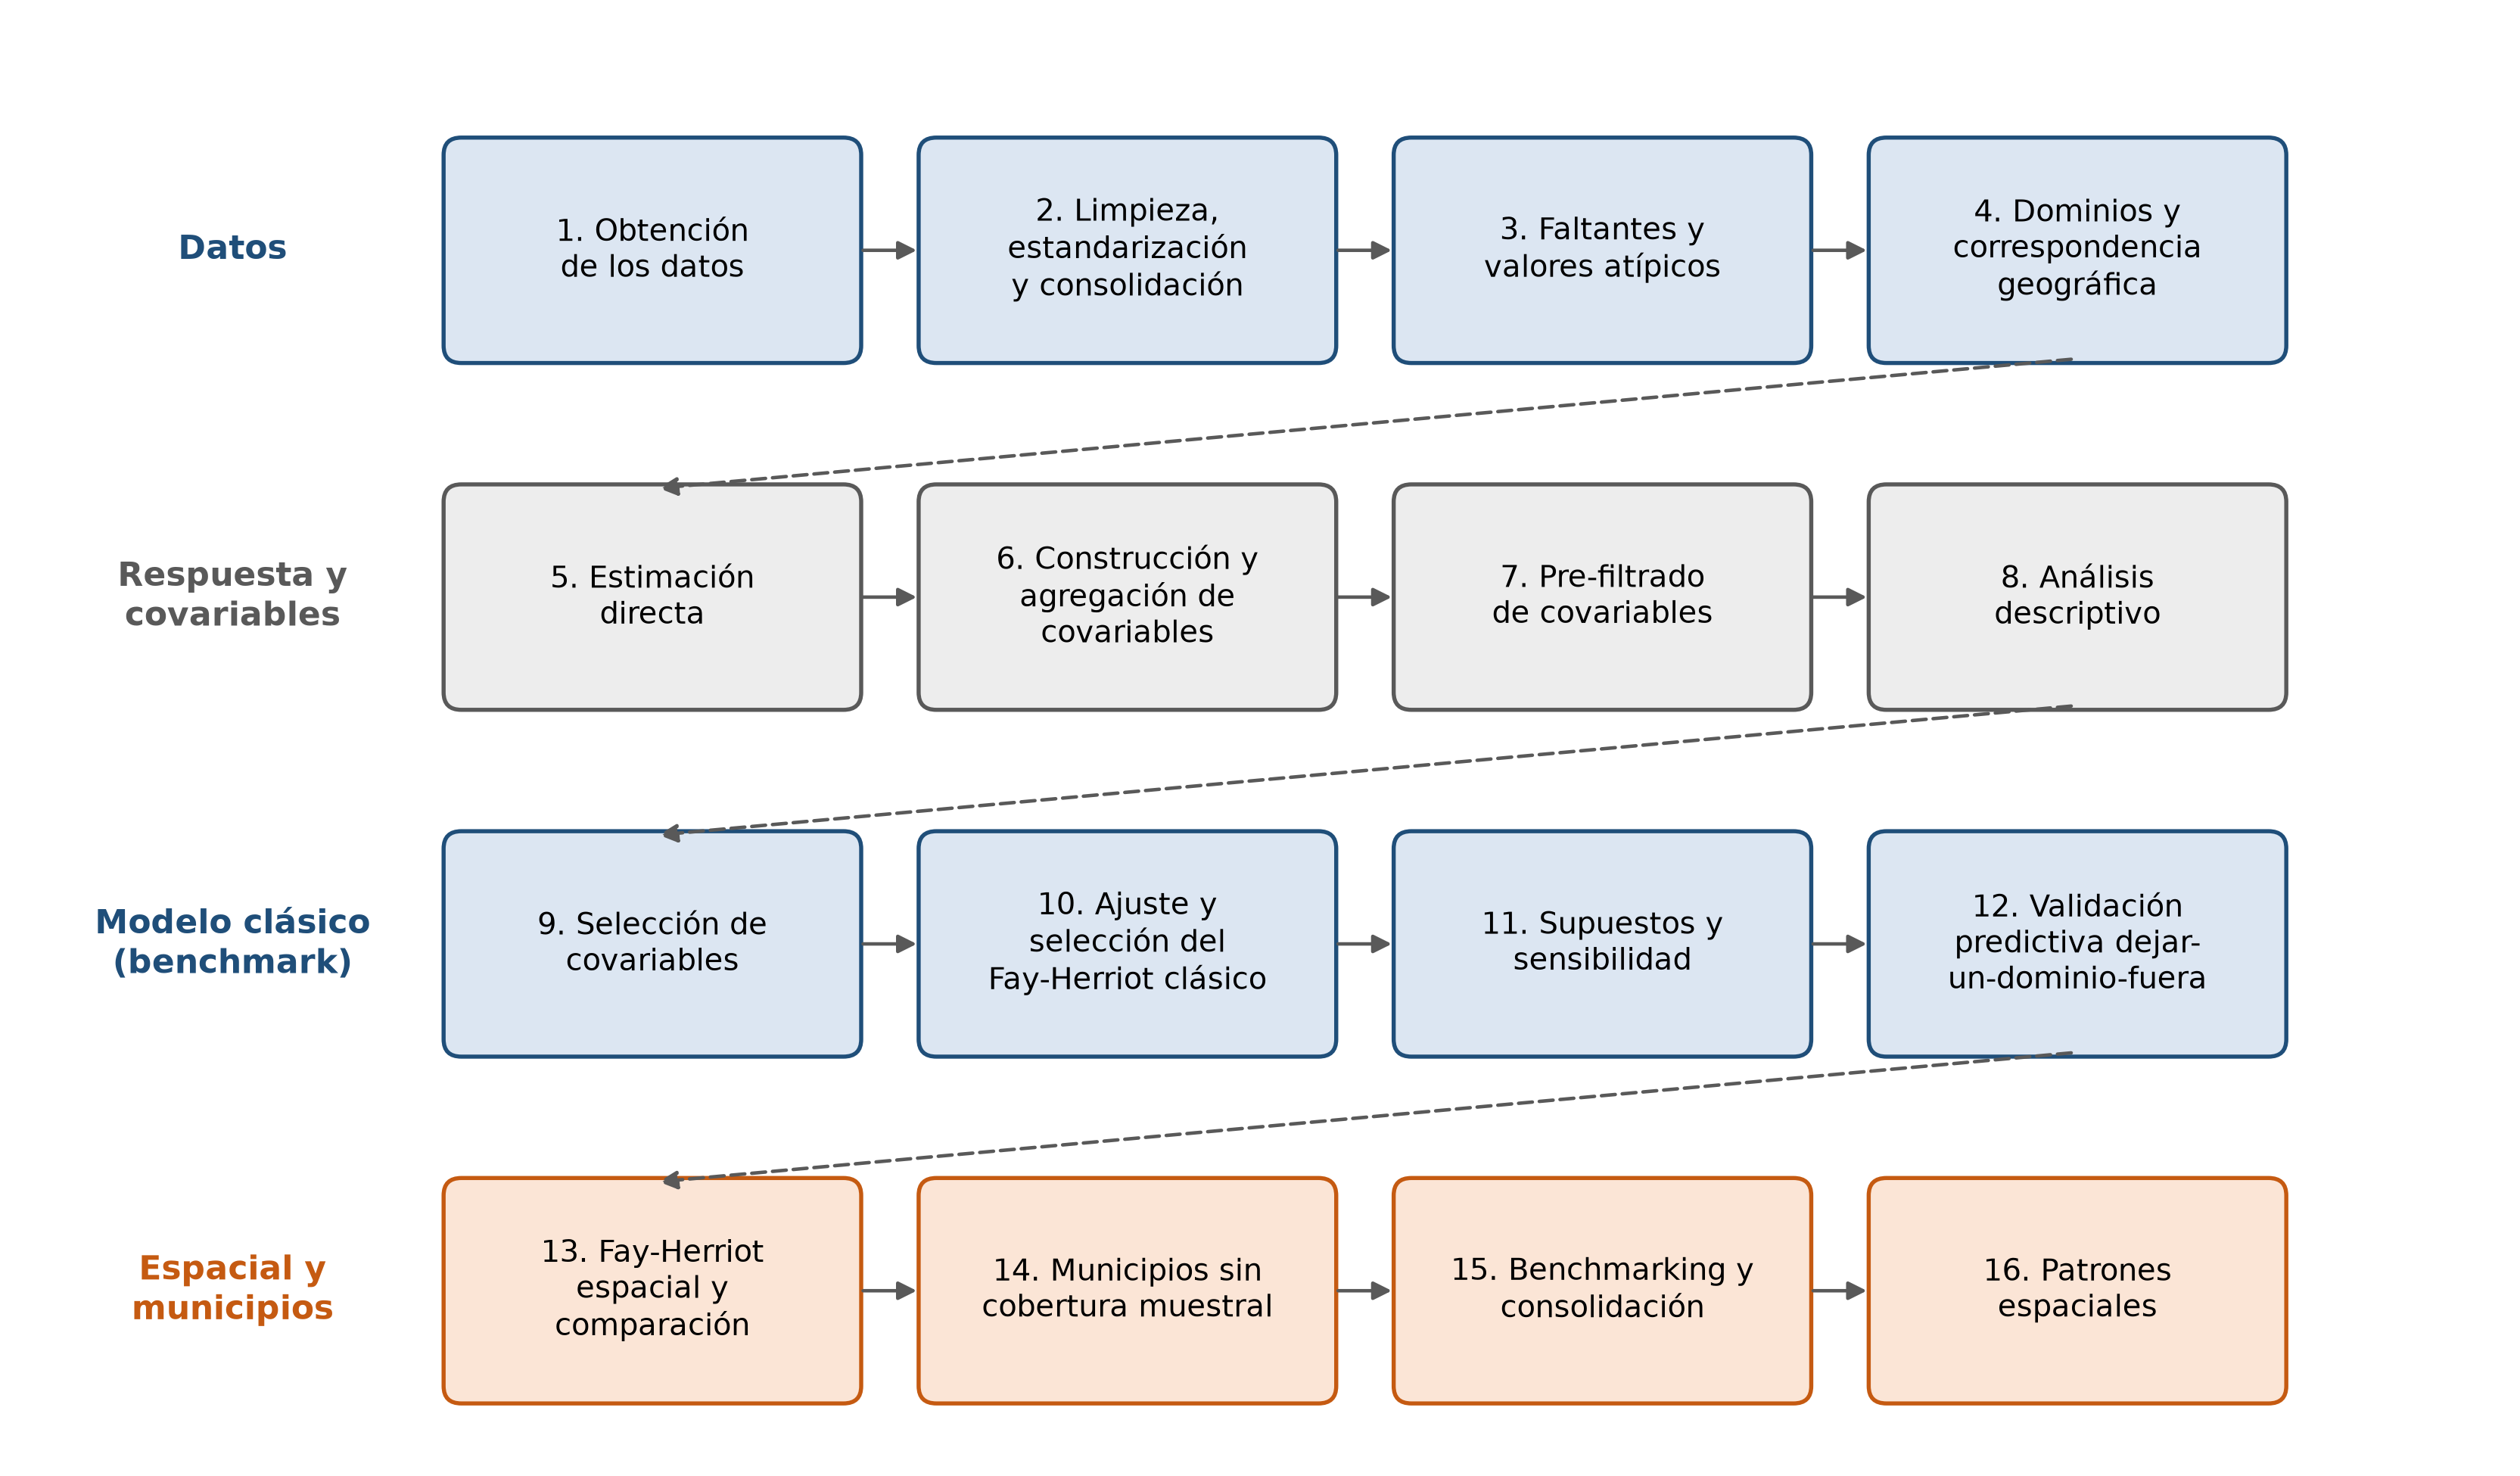
\includegraphics[width=\linewidth]{img/met_flujo_general.png}
\caption{Etapas de la metodología. Las flechas continuas unen etapas de una misma fase y las discontinuas el paso de una fase a la siguiente. Cada etapa tiene una sección con el mismo número en este capítulo y en Resultados.}
\label{fig:met_flujo}
\end{figure}

Cada etapa se presenta con una ficha que reúne sus entradas, las transformaciones, la regla de decisión, los parámetros fijados de antemano, el sustento y la salida. Todo el procesamiento corrió en Databricks, con tablas en un catálogo de Unity Catalog organizado en capas, y se despliega como un conjunto de trabajos programados que repiten la cadena completa; el linaje de tablas y la forma de reproducir cada etapa están en el Apéndice~\ref{app:reproducibilidad}.

%--------------------------------------------------------------------------------------
\section{Obtención de los datos}
\label{sec:met_obtencion}

Las cuatro fuentes de la Sección~\ref{sec:datos} se cargaron sin modificar su contenido, siguiendo una arquitectura de medallón: una capa bronce con los datos como llegan, una capa plata con los datos limpios y consolidados, y una capa oro con la tabla analítica de mercado laboral (Tabla~\ref{tab:met_obtencion}). La capa bronce permite repetir cualquier transformación posterior sin volver a descargar las fuentes.

\begin{table}[!htbp]
\centering
\small
\caption{Ficha de la etapa 1: obtención de los datos.}
\label{tab:met_obtencion}
\renewcommand{\arraystretch}{1.15}
\begin{tabularx}{\linewidth}{>{\raggedright\arraybackslash}p{2.8cm} >{\raggedright\arraybackslash}X}
\toprule
Elemento & Contenido \\
\midrule
Entradas & Archivos de texto de la GEIH 2018 por mes, módulo y sección (cabecera y resto); archivo de factores de expansión recalculados con el CNPV 2018; archivos de TerriData en formato largo; DIVIPOLA; hojas del anexo del DANE \\
Transformaciones & Lectura de cada archivo por separado y unión por nombre de columna; columna con el archivo de origen de cada registro; ningún valor se modifica \\
Regla de decisión & Se cargan solo los módulos necesarios para la condición de actividad (Tabla~\ref{tab:dimensiones-geih-modulos}) \\
Sustento & Definiciones de la encuesta \cite[p.~20]{DANE_GEIH_Metodologia2016} \\
Salida & Capa bronce: una tabla por módulo y sección de la GEIH, una para TerriData y una por hoja del anexo \\
\bottomrule
\end{tabularx}
\end{table}

%--------------------------------------------------------------------------------------
\section{Limpieza, estandarización y consolidación}
\label{sec:met_limpieza}

La GEIH reparte la información de una persona en varios módulos, y en el marco antiguo cada módulo en dos archivos. Esta etapa los une en una tabla con una fila por persona y verifica que la clasificación resultante sea coherente (Tabla~\ref{tab:met_limpieza}). La llave de una persona es la concatenación del período, la vivienda, el hogar y el orden dentro del hogar; la vivienda (período y directorio) se conserva aparte porque es la unidad del bootstrap de la etapa 5.

Dos correcciones de esta etapa cambian las cifras y por eso se describen. Primero, los archivos de enero a marzo de 2018 traen las columnas en otro orden; leerlos todos a la vez asignaba los valores por posición, corría las columnas y dejaba a toda la población en edad de trabajar como activa. Se leyó cada archivo por separado y se unieron por nombre de columna. Segundo, en el marco antiguo el factor de expansión sale solo del archivo recalculado con el CNPV 2018; si una persona queda sin factor o con factor no positivo, el procesamiento se detiene antes de escribir la tabla, en lugar de asignarle cero.

\begin{table}[!htbp]
\centering
\small
\caption{Ficha de la etapa 2: limpieza, estandarización y consolidación.}
\label{tab:met_limpieza}
\renewcommand{\arraystretch}{1.15}
\begin{tabularx}{\linewidth}{>{\raggedright\arraybackslash}p{2.8cm} >{\raggedright\arraybackslash}X}
\toprule
Elemento & Contenido \\
\midrule
Entradas & Capa bronce de la GEIH (identificadores de texto, indicadores binarios de condición, edad entera, factor de expansión continuo) \\
Transformaciones & Nombres de columna y tipos comunes a ambos marcos; separador decimal; unión de cabecera y resto; PEA del marco antiguo como la PET que no figura entre los inactivos; unión de los módulos a características generales por la llave de persona; factor de expansión por marco; código de municipio del área y nombre del departamento desde las tablas de dimensión \\
Regla de decisión & El procesamiento se detiene si alguna persona queda sin factor de expansión o con factor no positivo \\
Verificaciones & Porcentaje de llaves de cada módulo sin pareja en características generales; identidades PEA = OC + DS y PET = PEA + PEI (Ecuación~\ref{eq:identidades}) por año, mes y dominio, con la cuenta de los casos que las rompen; personas sin factor \\
Sustento & Factores CNPV 2018 y salto de serie al mezclar factores \cite[pp.~3, 19]{DANE_GEIH_Series2022} \\
Salida & Tabla de mercado laboral (capa oro) y tablas de reconciliación \\
\bottomrule
\end{tabularx}
\end{table}

En TerriData la limpieza normalizó los nombres de departamento y entidad (mayúsculas y sin tildes), unificó el valor numérico y el cualitativo en un solo campo, clasificó cada indicador como numérico si al menos el 95~\% de sus registros es numérico, y pasó la base a formato ancho, con una fila por entidad, año y mes y una columna por indicador. Cuatro comprobaciones (número de filas antes y después, duplicados de la llave, una muestra aleatoria comparada en ambos formatos y el total de valores no nulos) se imprimen como aprobadas o no, sin detener el proceso.

%--------------------------------------------------------------------------------------
\section{Tratamiento de datos faltantes y valores atípicos}
\label{sec:met_faltantes}

La Tabla~\ref{tab:met_faltantes} reúne qué se hizo con los faltantes y los atípicos según el papel de cada variable. No se imputó ningún valor: los indicadores de condición de actividad se construyen por la pertenencia a un módulo, el factor de expansión faltante detiene el procesamiento y una covariable incompleta queda fuera del modelo. Tampoco se eliminaron dominios ni municipios por ser atípicos: con 23 dominios, cada uno es un territorio real, y su influencia se mide con la distancia de Cook y con el reajuste sin cada dominio (etapa 11).

\begin{table}[!htbp]
\centering
\small
\caption{Ficha de la etapa 3: tratamiento de datos faltantes y valores atípicos.}
\label{tab:met_faltantes}
\renewcommand{\arraystretch}{1.15}
\begin{tabularx}{\linewidth}{>{\raggedright\arraybackslash}p{3.2cm} >{\raggedright\arraybackslash}X}
\toprule
Variable o caso & Tratamiento \\
\midrule
Condición de actividad (PET, PEA, OC, DS, PEI) & Es 1 si la persona está en el módulo que la define y 0 si no; la ausencia en el módulo de ocupados, por ejemplo, significa que no está ocupada \\
Factor de expansión & Sin imputación: si falta o no es positivo, el procesamiento se detiene (etapa 2) \\
Registros sin código de área & No se usan: no pertenecen a ninguno de los 23 dominios (Sección~\ref{sec:datos_geih}) \\
Covariable con faltantes en los dominios & Sale en el pre-filtrado (etapa 7) \\
Covariable con faltantes en los municipios objetivo & No entra al catálogo activo: sin ella no hay estimación sintética (etapa 6) \\
Valores no interpretables en TerriData & Se convierten a nulo y siguen la regla anterior \\
Valores atípicos & No se eliminan ni se recortan; se señalan con la regla del diagrama de caja (Ecuación~\ref{eq:iqr}) y su influencia se mide en la etapa 11 \\
\bottomrule
\end{tabularx}
\end{table}

Algunos criterios habituales no aplican. No hay covariables categóricas ni codificación de variables indicadoras: las 18 candidatas son cuantitativas. No hay una búsqueda de hiperparámetros: los parámetros del procedimiento (umbrales, réplicas, semillas) se fijaron antes de ver los resultados, y en el modelo espacial se comparan cuatro matrices de proximidad como escenarios, no como valores para optimizar.

%--------------------------------------------------------------------------------------
\section{Definición de los dominios de estimación y correspondencia geográfica}
\label{sec:met_dominios}

El dominio de estimación es la unidad que identifica la GEIH: la ciudad capital o la ciudad con su área metropolitana. Así, la tasa directa de Cali es la de Cali A.M., la misma unidad para la que publica el DANE. Cada dominio lleva el código DIVIPOLA de su capital, y una tabla de dimensión enumera sus municipios miembro con la composición de la metodología de la encuesta (Tabla~\ref{tab:met_dominios}). Una tabla de auditoría documenta, para cada dominio, el período, el código de área de la GEIH, el nombre con que lo publica el DANE, la geografía de la tasa (las cabeceras) y la de las covariables (el municipio completo), los municipios miembro con su código, la regla de agregación de las covariables y la tasa directa frente a la del DANE en la misma ventana.

\begin{table}[!htbp]
\centering
\small
\caption{Ficha de la etapa 4: definición de los dominios y correspondencia geográfica.}
\label{tab:met_dominios}
\renewcommand{\arraystretch}{1.15}
\begin{tabularx}{\linewidth}{>{\raggedright\arraybackslash}p{2.8cm} >{\raggedright\arraybackslash}X}
\toprule
Elemento & Contenido \\
\midrule
Entradas & Código de área de la GEIH; DIVIPOLA; lista de capitales y de municipios de cada área metropolitana \\
Transformaciones & Código de área $\to$ código del departamento de la capital $\to$ código DIVIPOLA de la capital; una fila por municipio miembro con el dominio al que pertenece y su tipo (ciudad o ciudad con A.M.) \\
Regla de decisión & Membresía estricta de la GEIH; los registros sin código de área no se usan \\
Sustento & Composición de las áreas metropolitanas \cite[p.~9]{DANE_GEIH_Metodologia2016} \\
Salida & Tabla de dominios (32 capitales, 52 municipios miembro; 23 dominios con muestra en 2018) y tabla de auditoría de los 23 dominios \\
\bottomrule
\end{tabularx}
\end{table}

%--------------------------------------------------------------------------------------
\section{Estimación directa de la tasa de desempleo}
\label{sec:met_directa}

La respuesta del modelo es la tasa directa de cada dominio en el año 2018, con la varianza que el modelo trata como conocida (Tabla~\ref{tab:met_directa}). La ventana de un año calendario se eligió frente al mes y al trimestre porque reúne más viviendas por dominio, lo que reduce la varianza de la estimación; la sensibilidad de la tasa a las tres ventanas se calculó aparte con el mismo estimador y no alimenta el modelo. El DANE no publica la tasa anual por ciudad, así que la cifra de referencia de cada dominio se reconstruye como la suma de desocupados sobre la suma de la PEA de los cuatro trimestres del año que no se superponen.

\begin{table}[!htbp]
\centering
\small
\caption{Ficha de la etapa 5: estimación directa.}
\label{tab:met_directa}
\renewcommand{\arraystretch}{1.15}
\begin{tabularx}{\linewidth}{>{\raggedright\arraybackslash}p{2.8cm} >{\raggedright\arraybackslash}X}
\toprule
Elemento & Contenido \\
\midrule
Entradas & Tabla de mercado laboral: indicador de desocupado (binario), factor de expansión (continuo), vivienda; personas de 15 años y más de la PEA en los 12 meses de 2018; tabla de dominios \\
Transformaciones & Estimador de Hájek por dominio (Ecuación~\ref{eq:hajek}); bootstrap por viviendas con el dominio como estrato (Ecuaciones~\ref{eq:var_bootstrap} y~\ref{eq:ic_bootstrap}); varianza de Taylor con las mismas viviendas (Ecuación~\ref{eq:taylor}); CV (Ecuación~\ref{eq:cve}); PEA expandida media mensual, peso del benchmarking \\
Regla de decisión & Clase del CV: confiable ($<5~\%$), aceptable ($5$ a $<20~\%$), no confiable ($\geq 20~\%$) \\
Parámetros & Ventana de 12 meses con cierre en diciembre (alternativa admitida: trimestre); $B = \num{2000}$ réplicas; semilla 42; edad mínima 15 años \\
Verificaciones & Tasa de cada dominio y tasa conjunta ponderada por la PEA frente a las del DANE en la misma ventana; bootstrap frente a Taylor \\
Sustento & \cite[pp.~21--22, 26--27, 61]{morales2021smallarea}; \cite[pp.~12, 15]{DANE_GEIH_Metodologia2016}; umbral del 20~\%: \cite[pp.~14--15]{Molina2019} \\
Salida & Por dominio: tasa, error estándar bootstrap, intervalo del 95~\%, CV y clase, error estándar de Taylor, personas, desocupados y viviendas de la muestra, PEA expandida \\
\bottomrule
\end{tabularx}
\end{table}

El bootstrap no reproduce el estrato interno ni el segmento, que no vienen en los microdatos. Por eso no se afirma que la varianza obtenida quede por encima ni por debajo de la del diseño, y la etapa 11 evalúa qué pasa con el modelo si se reemplaza.

%--------------------------------------------------------------------------------------
\section{Construcción y agregación de las covariables}
\label{sec:met_covariables}

Las covariables candidatas salen de un catálogo construido con la revisión de literatura del proyecto: entra un indicador solo si un estudio lo relaciona con el desempleo, y cada entrada declara el signo esperado de esa relación y su referencia, antes de calcular ninguna cifra (Tabla~\ref{tab:met_covariables}). La exigencia de una relación interpretable sigue la recomendación de que las variables auxiliares tengan una explicación acorde con la disciplina que estudia el fenómeno \cite[p.~453]{morales2021smallarea}. Las justificaciones del catálogo hablan de asociación, no de causa. El catálogo completo, con el código de TerriData y la referencia de cada entrada, está en el Apéndice~\ref{app:catalogo}.

\begin{table}[!htbp]
\centering
\small
\caption{Ficha de la etapa 6: construcción y agregación de las covariables.}
\label{tab:met_covariables}
\renewcommand{\arraystretch}{1.15}
\begin{tabularx}{\linewidth}{>{\raggedright\arraybackslash}p{2.8cm} >{\raggedright\arraybackslash}X}
\toprule
Elemento & Contenido \\
\midrule
Entradas & TerriData en formato ancho (indicadores cuantitativos: porcentajes, tasas, valores per cápita, puntajes); tabla de dominios; tasas directas \\
Transformaciones & Valor del dominio por razón de totales con el denominador propio de cada indicador (Ecuación~\ref{eq:agregacion}; denominadores en la Tabla~\ref{tab:covariables_datos}); unión con las tasas por dominio, año y mes; tabla de municipios objetivo con sus covariables a nivel municipal y, para Cali y Yumbo, el dominio al que pertenecen \\
Regla de decisión & Entrada activa si tiene referencia, dato para 2018 y valor en todos los municipios objetivo; toda covariable debe tener una regla de agregación, y el valor de un dominio es nulo si le falta a alguno de sus miembros \\
Parámetros & Departamentos objetivo: 19 (Cauca) y 76 (Valle del Cauca) \\
Verificaciones & Sensibilidad de las covariables de las 7 áreas metropolitanas a ponderar todas por la población de 15 años y más en lugar de su denominador propio; el procesamiento se detiene si a un miembro le falta un peso, si falta un miembro de un dominio con A.M. entre los objetivos o si no queda ningún municipio objetivo \\
Sustento & Valor del área \cite[p.~425]{morales2021smallarea}; razón de totales \cite[p.~21]{morales2021smallarea} \\
Salida & Catálogo (18 activas y 6 sin dato utilizable, con su motivo); tabla de 23 dominios con respuesta y covariables; tabla de 83 municipios objetivo \\
\bottomrule
\end{tabularx}
\end{table}

El índice de incidencia del conflicto armado, que estaba en una versión anterior del catálogo, se retiró: mide el conflicto en el propio municipio y no la llegada de población desplazada que motivaba su inclusión, toma 13 valores distintos por redondeo y tiene una correlación de 0.92 con la tasa de homicidios. No se sustituyó por otro indicador. La tasa de tránsito a la educación superior se conservó por decisión del equipo.

%--------------------------------------------------------------------------------------
\section{Pre-filtrado de covariables}
\label{sec:met_prefiltrado}

El pre-filtrado retira las candidatas que no se pueden usar, sin mirar su relación con la tasa de desempleo (Tabla~\ref{tab:met_prefiltrado}). Por eso no se repite dentro de la validación predictiva de la etapa 12.

\begin{table}[!htbp]
\centering
\small
\caption{Ficha de la etapa 7: pre-filtrado de covariables.}
\label{tab:met_prefiltrado}
\renewcommand{\arraystretch}{1.15}
\begin{tabularx}{\linewidth}{>{\raggedright\arraybackslash}p{2.8cm} >{\raggedright\arraybackslash}X}
\toprule
Elemento & Contenido \\
\midrule
Entradas & Tabla de 23 dominios con todas las columnas de TerriData del período \\
Transformaciones & Conversión numérica tolerante a errores de las columnas de texto \\
Regla de decisión & Completitud: sin faltantes en los 23 dominios. Variabilidad: CV descriptivo (Ecuación~\ref{eq:cv_descriptivo}) $\geq 0.001$ y proporción de dominios con el valor modal $\leq 0.90$. Sin filtro por correlación con la respuesta \\
Parámetros & CV mínimo 0.001; proporción modal máxima 0.90; los pares con $|r| \geq 0.999$ se reportan como duplicados, sin decidir \\
Verificaciones & Cascada (candidatas que pasan cada filtro) y sensibilidad del número de sobrevivientes a los dos umbrales de variabilidad \\
Sustento & Una columna constante es colineal con el intercepto y deja singular la matriz de la Ecuación~\ref{eq:gls}; los dos criterios no dependen de la unidad del indicador \\
Salida & Covariables pre-filtradas, cascada y sensibilidad \\
\bottomrule
\end{tabularx}
\end{table}

%--------------------------------------------------------------------------------------
\section{Análisis descriptivo}
\label{sec:met_descriptivo}

El análisis descriptivo caracteriza la tasa directa, su precisión y las candidatas activas, en tres niveles (Tabla~\ref{tab:met_descriptivo}). No decide: una variable asimétrica no se descarta por serlo y un dominio extremo no se retira. No se aplicó análisis de componentes principales, porque sus combinaciones no tienen una lectura territorial y exigen decidir cuántas retener. Tampoco se aplicó la prueba de Shapiro-Wilk a las covariables: el modelo supone normalidad de los efectos y de los errores, no de las covariables.

\begin{table}[!htbp]
\centering
\small
\caption{Ficha de la etapa 8: análisis descriptivo.}
\label{tab:met_descriptivo}
\renewcommand{\arraystretch}{1.15}
\begin{tabularx}{\linewidth}{>{\raggedright\arraybackslash}p{2.8cm} >{\raggedright\arraybackslash}X}
\toprule
Elemento & Contenido \\
\midrule
Entradas & Tasa directa, su error estándar y $\psi_d$; 18 candidatas activas; diccionario de indicadores \\
Univariado & Posición, dispersión, asimetría y CV descriptivo (Ecuación~\ref{eq:cv_descriptivo}); valores señalados por la regla del diagrama de caja (Ecuación~\ref{eq:iqr}) con el dominio al que corresponden; diagramas de caja en escala estandarizada (solo gráfica) \\
Bivariado & Pearson y Spearman con la tasa (Ecuaciones~\ref{eq:pearson} y~\ref{eq:spearman}) e intervalo de Fisher (Ecuación~\ref{eq:ic_fisher}); diagramas de dispersión \\
Multivariado & Matriz de correlaciones reordenada por agrupamiento de enlace promedio con la distancia de la Ecuación~\ref{eq:distancia_correlacion}; pares con $|r| > 0.80$ \\
Regla de decisión & Ninguna: la etapa es descriptiva \\
Salida & Tablas univariada y bivariada; figuras de la respuesta, de su distribución por dominio, de las candidatas y de sus correlaciones; interpretación calculada desde los datos \\
\bottomrule
\end{tabularx}
\end{table}

%--------------------------------------------------------------------------------------
\section{Selección de covariables}
\label{sec:met_seleccion}

La selección elige las covariables del modelo en cinco pasos (Tabla~\ref{tab:met_seleccion}). Cada paso se puede verificar por separado, y el recorrido de cada candidata queda registrado. Decide el modelo Fay-Herriot univariado con las mismas $\psi_d$ del modelo final, no la correlación de Pearson, porque el primero pondera cada dominio por la precisión de su estimación directa.

\begin{table}[!htbp]
\centering
\small
\caption{Ficha de la etapa 9: selección de covariables.}
\label{tab:met_seleccion}
\renewcommand{\arraystretch}{1.15}
\begin{tabularx}{\linewidth}{>{\raggedright\arraybackslash}p{2.8cm} >{\raggedright\arraybackslash}X}
\toprule
Paso & Contenido \\
\midrule
1. Asociación & Fay-Herriot univariado por candidata (REML y GLS), con intervalo de Wald de $\beta_1$, valor $p$ y correlación ponderada $r_w$ (Ecuación~\ref{eq:r_ponderada}), que ordena y fija el signo; valor $q$ de Benjamini-Hochberg sobre las 18 (Ecuación~\ref{eq:bh}). Forma funcional como diagnóstico: término cuadrático y logaritmo frente a lineal por AIC \\
2. Robustez y soporte & Diagnósticos, no filtros: Cook (Ecuación~\ref{eq:cook}) y cambio de $r_w$ al retirar cada dominio (dependencia si Cook $> 4/n$ y el cambio supera 0.10 o invierte el signo); proporción de municipios objetivo dentro del rango de los dominios, con advertencia por debajo de 0.80 \\
3. Redundancia & Grupos por enlace completo con $|r| \geq 0.80$ entre todos sus pares; representante: el primer integrante elegible con menor Cook máximo; si no es elegible, se pasa al siguiente \\
4. Ficha de decisión & Elegible si $q \leq 0.10$; el signo esperado se compara con el observado como diagnóstico; se seleccionan las $\lfloor n/10 \rfloor$ elegibles de mayor $|r_w|$ (Ecuación~\ref{eq:pmax}); si no hay elegibles, el conjunto queda vacío y el modelo usa solo el intercepto \\
5. Verificación & VIF del conjunto (Ecuación~\ref{eq:vif}); si una supera 5, se reemplaza por la siguiente elegible; residuos parciales; repetición de la selección exigiendo el signo esperado, como sensibilidad \\
Parámetros & $q \leq 0.10$; $|r| \geq 0.80$; 10 observaciones por parámetro; VIF $\leq 5$; Cook $4/n$ y cambio 0.10 (inspección); soporte 0.80 (advertencia) \\
Sustento & \cite[pp.~453--454]{morales2021smallarea}; \cite{BenjaminiHochberg1995}; VIF: \cite[sec.~9.4]{MontgomeryPeckVining2012}; cota, 0.80 y $4/n$: convenciones del trabajo \\
Salida & Diagnósticos por candidata, grupos de redundancia, ficha de decisión, verificación, trazabilidad y conjunto seleccionado \\
\bottomrule
\end{tabularx}
\end{table}

En una versión anterior, la robustez descartaba candidatas. Se cambió a diagnóstico porque la regla $4/n$ sirve para inspeccionar observaciones, no para excluir variables, y porque el umbral de 0.10 en el cambio de la correlación queda por debajo del error de muestreo de $r$ con 23 dominios; la literatura de referencia no usa la influencia para seleccionar \cite[pp.~453--454]{morales2021smallarea}. No se hizo una búsqueda exhaustiva de especificaciones por AIC entre las 18 candidatas: con 23 dominios produciría muchas especificaciones equivalentes y reutilizaría los mismos datos que ajustan el modelo.

%--------------------------------------------------------------------------------------
\section{Ajuste y selección del modelo Fay-Herriot clásico (benchmark)}
\label{sec:met_fh_clasico}

Con el conjunto seleccionado se ajustan varias especificaciones candidatas del modelo base Fay-Herriot clásico y se elige una, que es el benchmark no espacial contra el que se compara el modelo espacial (Tabla~\ref{tab:met_fh_clasico}). Las especificaciones se nombran EC1 (el conjunto seleccionado), EC2, EC3 y siguientes (sus subconjuntos no vacíos) y EC0 (solo intercepto). No son los modelos finales del objetivo específico 1: son las variantes entre las que se elige el benchmark.

\begin{table}[!htbp]
\centering
\small
\caption{Ficha de la etapa 10: ajuste y selección del Fay-Herriot clásico.}
\label{tab:met_fh_clasico}
\renewcommand{\arraystretch}{1.15}
\begin{tabularx}{\linewidth}{>{\raggedright\arraybackslash}p{2.8cm} >{\raggedright\arraybackslash}X}
\toprule
Elemento & Contenido \\
\midrule
Entradas & Tasa directa $\hat{\theta}_d$ y $\psi_d$ de los 23 dominios; covariables seleccionadas \\
Transformaciones & Para cada especificación: $\hat{\sigma}_u^2$ por REML, $\hat{\boldsymbol{\beta}}$ por GLS (Ecuación~\ref{eq:gls}), EBLUP (Ecuación~\ref{eq:eblup_a}), ECM de Prasad-Rao (Ecuaciones~\ref{eq:ecm_eblup} y~\ref{eq:ecm_componentes}), CV, AIC y AICc con la verosimilitud ML (Ecuaciones~\ref{eq:loglik} y~\ref{eq:aic}); error de estimación dejar-un-dominio-fuera de cada especificación, como descripción \\
Regla de decisión & Compiten las especificaciones con todas sus covariables con $p < 0.05$ (EC0 cumple de forma trivial); entre ellas, la de menor AIC, y entre las que difieren en $\Delta\text{AIC} \leq 2$, la de menos covariables. Si ninguna con covariables cumple, compiten todas y la elección se reporta como excepción \\
Parámetros & $\alpha = 0.05$; $\Delta\text{AIC} \leq 2$; aviso si $\max_d \hat{\gamma}_d < 0.01$ ($\hat{\sigma}_u^2 \approx 0$) o si alguna tasa cae fuera de $[0, 100]$ \\
Sustento & \cite[pp.~427, 434--441, 453--454]{morales2021smallarea}; AICc: \cite{HurvichTsai1989}; $\Delta\text{AIC} \leq 2$: convención \\
Salida & Diagnósticos y coeficientes de cada especificación; tabla de selección con el criterio aplicado; EBLUP, ECM, CV y $\hat{\gamma}_d$ de los 23 dominios con el benchmark \\
\bottomrule
\end{tabularx}
\end{table}

Los valores $p$ de esta etapa son descriptivos. Los mismos 23 dominios filtran las candidatas, las seleccionan y estiman los coeficientes, así que los coeficientes son asociaciones condicionales a la selección y no se interpretan como efectos causales. La literatura de referencia no trata este punto; el trabajo lo reporta como una limitación y lo examina en las etapas 11 y 12. El ECM y la distancia de Cook no intervienen en la elección: se reportan para el benchmark.

%--------------------------------------------------------------------------------------
\section{Validación de supuestos y sensibilidad del benchmark}
\label{sec:met_supuestos}

Esta etapa revisa los supuestos del benchmark y mide cuánto cambian sus coeficientes y sus estimaciones cuando cambian los datos o la varianza de muestreo (Tabla~\ref{tab:met_supuestos}). Ninguno de estos análisis cambia el modelo elegido ni las tasas publicadas.

\begin{table}[!htbp]
\centering
\small
\caption{Ficha de la etapa 11: validación de supuestos y sensibilidad del benchmark.}
\label{tab:met_supuestos}
\renewcommand{\arraystretch}{1.15}
\begin{tabularx}{\linewidth}{>{\raggedright\arraybackslash}p{2.8cm} >{\raggedright\arraybackslash}X}
\toprule
Análisis & Contenido \\
\midrule
Normalidad & Residuos estandarizados (Ecuación~\ref{eq:residuos}): media (cercana a cero por construcción), desviación, histograma y Shapiro-Wilk (Ecuación~\ref{eq:shapiro}), leído como «sin evidencia fuerte en contra», no como prueba de normalidad \\
Influencia & Distancia de Cook (Ecuación~\ref{eq:cook}) con $\hat{\sigma}_u^2$ fijo; reajuste sin el dominio más influyente \\
Estabilidad de coeficientes & 23 reajustes dejando un dominio fuera (reestimando $\hat{\sigma}_u^2$): mínimo y máximo de cada $\hat{\beta}_j$, dominio que los produce, cambio estandarizado (Ecuación~\ref{eq:dfbeta}), cambios de signo y de significancia; efecto en los EBLUP de los otros dominios, en las estimaciones de los 83 municipios y en su clase de confiabilidad. Bootstrap de dominios con la especificación fija \\
Varianza de muestreo & Varianzas alternativas: bootstrap por personas, Taylor, GVF A y B (Ecuación~\ref{eq:gvf}); nueve escenarios del modelo: base, Taylor, GVF A y $\psi_d \times k$; en cada uno se reajustan todas las especificaciones y se vuelve a elegir con la misma regla; se comparan $\hat{\sigma}_u^2/\bar{\psi}$, $\hat{\gamma}_d$, $\hat{\boldsymbol{\beta}}$, EBLUP, CV, clase, $\lambda_1$ y estimaciones municipales \\
Parámetros & Umbrales de influencia: 1 error estándar y 0.5 puntos porcentuales; \num{1000} réplicas bootstrap, semilla 42; $k \in \{1/3, 1/2, 2/3, 3/2, 2, 3\}$ \\
Sustento & \cite{ShapiroWilk1965, Cook1977}; GVF: \cite[p.~427]{morales2021smallarea}, \cite[pp.~15--16]{MarinTralmaGuerrero2024}, \cite[p.~15]{Tellez2020}; $\hat{\sigma}_u^2/\bar{\psi}$: \cite[p.~143]{Benedetti2024}; umbrales de influencia: convención \\
Salida & Tablas de estabilidad, de influencia por dominio y de escenarios de varianza; mapa de calor de la influencia \\
\bottomrule
\end{tabularx}
\end{table}

%--------------------------------------------------------------------------------------
\section{Validación predictiva dejar-un-dominio-fuera}
\label{sec:met_validacion}

Las cifras del ajuste con los 23 dominios no dicen qué tan bien estima el modelo un lugar sin encuesta, porque el EBLUP de un dominio se apoya en su propia estimación directa. La validación predictiva dejar-un-dominio-fuera imita ese uso: retira un dominio, ajusta con los otros 22 y lo estima como si no tuviera encuesta (Tabla~\ref{tab:met_validacion}). Se hace de dos formas. Con las covariables del benchmark fijas, solo se reestiman $\hat{\boldsymbol{\beta}}$ y $\hat{\sigma}_u^2$; es optimista, porque esas covariables se eligieron viendo al dominio retirado. Con el procedimiento completo, en cada iteración se repiten la selección de la etapa 9 y la elección de la etapa 10 con los 22 dominios que quedan. La diferencia entre ambos errores es el costo de haber seleccionado con los mismos datos.

\begin{table}[!htbp]
\centering
\small
\caption{Ficha de la etapa 12: validación predictiva dejar-un-dominio-fuera.}
\label{tab:met_validacion}
\renewcommand{\arraystretch}{1.15}
\begin{tabularx}{\linewidth}{>{\raggedright\arraybackslash}p{2.8cm} >{\raggedright\arraybackslash}X}
\toprule
Elemento & Contenido \\
\midrule
Entradas & 23 dominios con respuesta, $\psi_d$ y las 18 candidatas pre-filtradas; benchmark de la etapa 10 \\
Transformaciones & Para cada dominio: ajuste sin él y estimación sintética $\mathbf{x}_d^\top\hat{\boldsymbol{\beta}}_{(-d)}$ con tres especificaciones: covariables fijas, procedimiento completo y solo intercepto (referencia) \\
Métricas & RMSE, MAE, sesgo, RMSE corregida por ruido, $Z_\psi$, $Z_{\text{pred}}$ (media, desviación y cobertura) y habilidad frente al modelo de solo intercepto (Ecuación~\ref{eq:metricas_val}); error dentro de muestra para medir el optimismo; conjunto elegido en cada iteración y frecuencia de cada covariable \\
Regla de decisión & Ninguna: la validación no cambia el benchmark. Si el procedimiento completo estima peor que el modelo de solo intercepto (habilidad negativa), se reporta como limitación, con la inestabilidad del conjunto entre iteraciones \\
Verificaciones & Con los 23 dominios, la selección y la elección deben reproducir el conjunto y el benchmark; si no, se advierte y se sigue \\
Parámetros & Cobertura nominal del 95~\% \\
Sustento & Análisis propio; lectura del estimador fuera de muestra: \cite[p.~441]{morales2021smallarea}, \cite[p.~144]{Benedetti2024} \\
Salida & Errores por dominio y ejercicio, métricas por ejercicio, selección por iteración y frecuencia de selección \\
\bottomrule
\end{tabularx}
\end{table}

Con 23 dominios las métricas resultan de 23 estimaciones y se leen como orden de magnitud.

%--------------------------------------------------------------------------------------
\section{Modelo Fay-Herriot espacial y comparación con el benchmark}
\label{sec:met_espacial}

El objetivo específico 1 compara el benchmark con especificaciones espaciales. La comparación es controlada: misma respuesta, mismas $\psi_d$, mismos 23 dominios y las mismas covariables del benchmark, sin volver a seleccionarlas. Cambia solo la estructura de los efectos de área (Ecuación~\ref{eq:sar}). La Tabla~\ref{tab:met_espacial} es la ficha de la etapa y la Tabla~\ref{tab:met_comparacion}, el contenido de la comparación.

\begin{table}[!htbp]
\centering
\small
\caption{Ficha de la etapa 13: modelo Fay-Herriot espacial y comparación con el benchmark.}
\label{tab:met_espacial}
\renewcommand{\arraystretch}{1.15}
\begin{tabularx}{\linewidth}{>{\raggedright\arraybackslash}p{2.8cm} >{\raggedright\arraybackslash}X}
\toprule
Elemento & Contenido \\
\midrule
Entradas & Las mismas del benchmark, más las coordenadas de las cabeceras de los 23 dominios y de los 83 municipios objetivo \\
Matriz de proximidad & Distancia de gran círculo entre cabeceras; cada dominio con A.M. es un solo nodo, ubicado en su capital; cuatro escenarios: 3 y 5 vecinos más cercanos, distancia inversa con potencia 1 y 2; estandarización por filas \\
Estructuras & «Muestra»: solo los 23 dominios. «Completa»: dominios y municipios objetivo, con verosimilitud marginal de los dominios. Ocho especificaciones en total \\
Estimación & $\hat{\sigma}_u^2$ y $\hat{\rho}$ por REML; AIC con ML; LRT de $\rho = 0$ (Ecuación~\ref{eq:lrt}); perfil de verosimilitud de $\rho$; SEBLUP (Ecuación~\ref{eq:seblup}); ECM por bootstrap paramétrico \\
Regla de decisión & Escenario de referencia: menor AIC entre las estructuras «completa» con $|\hat{\rho}| < 0.99$. El espacial se prefiere al clásico solo si $p(\text{LRT}) < 0.05$ en la estructura «muestra» del mismo escenario. El $\Delta$AIC y la validación se reportan, no deciden \\
Parámetros & $k \in \{3, 5\}$; potencias $\{1, 2\}$; $|\rho| \leq 0.99$; 500 réplicas bootstrap, semilla 42; \num{9999} permutaciones para Moran; $\alpha = 0.05$ \\
Sensibilidades & Ubicación del nodo de un A.M. en la media de sus municipios en lugar de la capital; $\hat{\rho}$ de la estructura «completa» con distintos conjuntos de municipios objetivo \\
Sustento & \cite[pp.~490--494]{morales2021smallarea}; \cite[pp.~146--149]{Benedetti2024}; \cite{PetrucciSalvati2006, PratesiSalvati2008}; escenarios de la matriz: convención \\
Salida & Comparación de especificaciones, cuadro comparativo, Moran, perfil de $\rho$, validación, coeficientes y sensibilidades \\
\bottomrule
\end{tabularx}
\end{table}

La vecindad se define por distancia y no por contigüidad porque los 23 dominios son ciudades dispersas y los municipios objetivo no limitan con ellas. El valor de $k$ y la potencia no los identifican los datos: $k = 3$ es la conexión mínima con la que ninguna ciudad queda aislada; con $k > 5$ y 23 nodos la matriz deja de ser local; la potencia 1 decae despacio y la 2 concentra el peso en las ciudades cercanas. Por eso se reportan los cuatro escenarios. El $\hat{\rho}$ de la estructura «completa» depende de qué municipios sin dato se incluyen como nodos, por lo que su signo no se interpreta y la prueba de $\rho = 0$ se hace en la estructura «muestra».

\begin{table}[!htbp]
\centering
\small
\caption{Contenido de la comparación entre el benchmark y el modelo espacial. Las diferencias se reportan sin pruebas adicionales al LRT de $\rho = 0$: con 23 dominios se describen, no se prueban.}
\label{tab:met_comparacion}
\renewcommand{\arraystretch}{1.15}
\begin{tabularx}{\linewidth}{>{\raggedright\arraybackslash}p{2.6cm} >{\raggedright\arraybackslash}X >{\raggedright\arraybackslash}p{2.6cm}}
\toprule
Elemento & Qué se compara & Ecuaciones \\
\midrule
Ajuste & $\hat{\sigma}_u^2$, $\hat{\rho}$, AIC, $\Delta$AIC y LRT del benchmark y de las ocho especificaciones espaciales & \ref{eq:aic}, \ref{eq:lrt} \\
Residuos & I de Moran de los residuos del clásico y del SEBLUP con la misma matriz y la misma estandarización; mapa de residuos & \ref{eq:moran} \\
Fuera de muestra & Validación dejar-un-dominio-fuera con covariables fijas para el sintético clásico, el sintético espacial y el espacial con efecto, con las métricas de la etapa 12 & \ref{eq:metricas_val} \\
Incertidumbre & ECM y CV del EBLUP y del SEBLUP en los 23 dominios; peso de la directa $\hat{\gamma}_d$ y $\hat{\gamma}^{S}_d$; ECM y CV de las estimaciones de los 83 municipios & \ref{eq:ecm_eblup}, \ref{eq:gamma_esp}, \ref{eq:var_sintetica} \\
Estimaciones & Diferencia en puntos porcentuales entre ambas estimaciones en dominios y municipios: media, máximo absoluto, correlación de Pearson y de Spearman; municipios que cambian de clase de confiabilidad & \ref{eq:pearson}, \ref{eq:spearman}, \ref{eq:cve} \\
Coeficientes & $\hat{\beta}_j$ y su error estándar en ambos modelos, y la diferencia medida en errores estándar del clásico & \ref{eq:gls} \\
\bottomrule
\end{tabularx}
\end{table}

Aparte de la comparación controlada, se reporta la comparación entre el benchmark, elegido con la regla de la etapa 10, y la especificación espacial de referencia, elegida con la regla de esta etapa entre los cuatro escenarios de la matriz.

%--------------------------------------------------------------------------------------
\section{Estimación en los municipios sin cobertura muestral}
\label{sec:met_sin_muestra}

Los 83 municipios objetivo reciben la estimación del modelo con sus propias covariables (Tabla~\ref{tab:met_sin_muestra}). En el clásico es el predictor sintético (Ecuación~\ref{eq:sintetico}); en el espacial, el predictor espacial (Ecuación~\ref{eq:pred_espacial}), que agrega el efecto que el modelo asigna a cada municipio a partir de los residuos de los dominios cercanos. Cali y Yumbo no son nodos de la matriz: forman parte del dominio Cali A.M. y reciben la parte sintética con sus propias covariables más el efecto estimado de su dominio. Cada estimación se acompaña de su estado de extrapolación y de una calidad reportada que no se reduce al CV.

\begin{table}[!htbp]
\centering
\small
\caption{Ficha de la etapa 14: estimación en los municipios sin cobertura muestral.}
\label{tab:met_sin_muestra}
\renewcommand{\arraystretch}{1.15}
\begin{tabularx}{\linewidth}{>{\raggedright\arraybackslash}p{2.8cm} >{\raggedright\arraybackslash}X}
\toprule
Elemento & Contenido \\
\midrule
Entradas & Covariables de los 83 municipios; $\hat{\boldsymbol{\beta}}$, $\widehat{\operatorname{Cov}}(\hat{\boldsymbol{\beta}})$ y $\hat{\sigma}_u^2$ del benchmark; ajuste espacial del escenario de referencia \\
Transformaciones & Predictor sintético y su ECM (Ecuaciones~\ref{eq:sintetico} y~\ref{eq:var_sintetica}); predictor espacial con ECM por bootstrap (nodos) o sintético (Cali y Yumbo); rango de cada covariable en los dominios y estado de extrapolación (Ecuación~\ref{eq:hnew}); estimación con covariables recortadas al rango y aporte extrapolado; reajuste sin cada dominio y amplitud de la estimación de cada municipio \\
Regla de decisión & Estado: fuera del rango, combinación atípica o dentro del rango. Calidad reportada: clase de CV, más «condicional al modelo» en todo municipio, más «extrapolado (fuera del rango)» o «extrapolado (combinación atípica)» si corresponde. La estimación publicada no cambia por la extrapolación \\
Sustento & \cite[pp.~3, 441--442, 453]{morales2021smallarea}; \cite[pp.~38--39]{Molina2019}; \cite[p.~144]{Benedetti2024}; \cite[sec.~3.8]{MontgomeryPeckVining2012} \\
Salida & Estimación de cada municipio con ambos modelos, ECM, CV, estado, covariable que más aporta a la extrapolación, aporte extrapolado, rangos y sensibilidad \\
\bottomrule
\end{tabularx}
\end{table}

%--------------------------------------------------------------------------------------
\section{Benchmarking y consolidación de las estimaciones}
\label{sec:met_benchmarking}

El benchmarking hace que las estimaciones del modelo reproduzcan cifras directas confiables de un territorio mayor, en dos niveles (Tabla~\ref{tab:met_benchmarking}). El resto de los municipios conserva la estimación sintética sin ajustar: el departamento tiene estimación directa anual en la GEIH, pero se calcula con los registros sin código de área, que este trabajo no usa; un tercer nivel departamental queda como extensión posible.

\begin{table}[!htbp]
\centering
\small
\caption{Ficha de la etapa 15: benchmarking y consolidación.}
\label{tab:met_benchmarking}
\renewcommand{\arraystretch}{1.15}
\begin{tabularx}{\linewidth}{>{\raggedright\arraybackslash}p{2.8cm} >{\raggedright\arraybackslash}X}
\toprule
Elemento & Contenido \\
\midrule
Entradas & EBLUP y ECM de los 23 dominios; PEA expandida de cada dominio; tasa directa del conjunto de los 23 dominios y cifra del DANE de la misma ventana; estimaciones de Cali y Yumbo y su población de 15 años y más \\
Nivel 1 & Factor $\lambda_1$ (Ecuación~\ref{eq:benchmarking}) para que los 23 EBLUP, ponderados por la PEA, reproduzcan la tasa conjunta \\
Nivel 2 & Factor $\lambda_D$ para que Cali y Yumbo, ponderados por su población de 15 años y más, reproduzcan el EBLUP ajustado de Cali A.M.; se reporta la brecha entre $\bar{\mathbf{x}}_D^\top\hat{\boldsymbol{\beta}}$ y el promedio ponderado de $\mathbf{x}_m^\top\hat{\boldsymbol{\beta}}$, porque las covariables del dominio no se agregan con la población de 15 años y más \\
Error & RMSE y CV ajustados (Ecuación~\ref{eq:rmse_bm}); la clase de confiabilidad se recalcula con el CV ajustado \\
Verificaciones & Consistencia (diferencia menor que $10^{-8}$), razones entre estimaciones conservadas, tasas en $[0, 100]$, miembros completos; aviso si $|\lambda - 1| > 0.20$ o si la tasa conjunta difiere de la del DANE en más de 0.01 puntos; repetición sobre la tabla final redondeada \\
Sustento & \cite{FayHerriot1979}; \cite[pp.~24, 76]{Molina2019}; \cite[pp.~22--23]{MarinTralmaGuerrero2024}; \cite[pp.~25, 33]{DANE_SAE_2025}; \cite[p.~7]{Casen2024} \\
Salida & Tabla final de dos niveles (23 dominios y 83 municipios) con tasa ajustada, tasa sin ajustar, factor, CV, clase, estado de extrapolación, calidad reportada, modelo de origen y estado preliminar \\
\bottomrule
\end{tabularx}
\end{table}

En la tabla final un mismo código puede aparecer como dominio y como municipio (76001 es Cali A.M. y también el municipio de Cali), por lo que la llave es el nivel más el código. Mientras no se cierre la comparación del objetivo específico 1, la tabla se marca como resultado preliminar del benchmark no espacial.

%--------------------------------------------------------------------------------------
\section{Distribución y patrones espaciales de las estimaciones}
\label{sec:met_patrones}

La última etapa describe dónde están las tasas altas y bajas en el Cauca y el Valle del Cauca y qué parte de ese patrón viene del modelo (Tabla~\ref{tab:met_patrones}). La lectura es descriptiva: las estimaciones municipales son funciones de las covariables, de modo que un patrón espacial en ellas refleja en buena parte la distribución espacial de esas covariables.

\begin{table}[!htbp]
\centering
\small
\caption{Ficha de la etapa 16: distribución y patrones espaciales de las estimaciones.}
\label{tab:met_patrones}
\renewcommand{\arraystretch}{1.15}
\begin{tabularx}{\linewidth}{>{\raggedright\arraybackslash}p{2.8cm} >{\raggedright\arraybackslash}X}
\toprule
Elemento & Contenido \\
\midrule
Entradas & Tabla final; estimaciones del espacial y su efecto por municipio; estado de extrapolación y calidad reportada; distancia de cada municipio al dominio más cercano; coordenadas \\
Transformaciones & Mapas municipales de la estimación, de su CV y calidad reportada, del estado de extrapolación y del efecto espacial; resumen por departamento; I de Moran de las 83 estimaciones con la matriz de 3 vecinos más cercanos (Ecuación~\ref{eq:moran}) \\
Regla de decisión & Ninguna: la etapa es descriptiva \\
Parámetros & Los de la etapa 13 para la matriz y las permutaciones \\
Sustento & Clústeres de desempleo municipal en Colombia \cite[pp.~123--124]{Diaz2016}; \cite{Moran1950} \\
Salida & Mapas y lectura territorial; índice de Moran de las estimaciones \\
\bottomrule
\end{tabularx}
\end{table}

%--------------------------------------------------------------------------------------
\section{Correspondencia entre etapas y objetivos}
\label{sec:met_objetivos}

La Tabla~\ref{tab:met_objetivos} relaciona cada etapa con el objetivo general (OG) y los objetivos específicos (OE1 a OE3), y con la evidencia que la responde en Resultados.

\begin{table}[!htbp]
\centering
\small
\caption{Etapa metodológica, objetivo al que responde y evidencia en Resultados. OG: objetivo general; OE: objetivo específico.}
\label{tab:met_objetivos}
\renewcommand{\arraystretch}{1.15}
\begin{tabularx}{\linewidth}{>{\raggedright\arraybackslash}p{4.4cm} >{\raggedright\arraybackslash}p{1.7cm} >{\raggedright\arraybackslash}X}
\toprule
Etapa & Objetivo & Evidencia en Resultados \\
\midrule
1--4. Datos, limpieza, faltantes y dominios & OG & Inventario de tablas, reconciliación y auditoría de dominios (Secciones~\ref{sec:res_obtencion} a~\ref{sec:res_dominios}) \\
5. Estimación directa & OG, OE1 & Tasas, CV y validación frente al DANE (Sección~\ref{sec:res_directa}) \\
6--8. Covariables, pre-filtrado y descriptivo & OG, OE2 & Catálogo, cascada y descripción de las candidatas (Secciones~\ref{sec:res_covariables} a~\ref{sec:res_descriptivo}) \\
9. Selección de covariables & OE2 & Ficha de decisión y conjunto seleccionado (Sección~\ref{sec:res_seleccion}) \\
10. Benchmark clásico & OE1, OE2 & Especificaciones, elección, coeficientes y EBLUP (Sección~\ref{sec:res_fh_clasico}) \\
11. Supuestos y sensibilidad & OE1, OE2 & Normalidad, influencia, estabilidad y escenarios de varianza (Sección~\ref{sec:res_supuestos}) \\
12. Validación predictiva & OE1, OE2 & Métricas de los dos ejercicios y frecuencia de selección (Sección~\ref{sec:res_validacion}) \\
13. Espacial y comparación & OE1, OE2, OE3 & Comparación controlada, Moran, validación y coeficientes (Sección~\ref{sec:res_espacial}) \\
14. Municipios sin cobertura & OG, OE3 & Estimaciones de los 83 municipios, extrapolación y calidad (Sección~\ref{sec:res_sin_muestra}) \\
15. Benchmarking y consolidación & OG & Factores, verificaciones y tabla final (Sección~\ref{sec:res_benchmarking}) \\
16. Patrones espaciales & OE3 & Mapas, efecto espacial y Moran de las estimaciones (Sección~\ref{sec:res_patrones}) \\
\bottomrule
\end{tabularx}
\end{table}

Los cuatro objetivos quedan cubiertos. El OE2 se responde como asociación estadística condicional a la selección, no como efecto causal, y su evidencia incluye la estabilidad del conjunto en la validación con el procedimiento completo.
\FloatBarrier

     % --------------------------
     \chapter{Resultados}
         
\label{sec:resultados}

Este capítulo presenta, etapa por etapa, lo que produjo el procedimiento de la Sección~\ref{sec:metodologia}, con los mismos títulos y en el mismo orden. Cada sección abre con la tabla o la figura que sirve de evidencia y la interpreta; los métodos y su sustento no se repiten. Todas las cifras corresponden a la corrida del año 2018 (ventana de enero a diciembre, 23 dominios y 83 municipios objetivo) y se leyeron de las tablas del procesamiento; las comparaciones entre el modelo clásico y el espacial que el procesamiento no guardaba se calcularon a partir de esas tablas, como se indica en la Sección~\ref{sec:res_espacial}. Las tablas largas y las figuras complementarias están en el Apéndice~\ref{app:resultados}; el nombre técnico de cada variable que el texto menciona en lenguaje natural, en el Apéndice~\ref{app:variables}.

%--------------------------------------------------------------------------------------
\section{Obtención de los datos}
\label{sec:res_obtencion}

La Tabla~\ref{tab:res_obtencion} resume lo que quedó cargado en cada capa. De la GEIH se cargaron los cinco módulos del marco antiguo para los doce meses de 2018 y dos meses de 2025 del marco nuevo, que se procesaron para comprobar que la cadena admite ambos marcos pero no entran en la estimación. TerriData llegó con más de 13 millones de registros en formato largo, que en la capa plata se convierten en una fila por entidad, año y mes. El linaje de las tablas, con el cuaderno que escribe cada una, está en el Apéndice~\ref{app:linaje}.

\begin{table}[!htbp]
\centering
\small
\caption{Volumen de datos por fuente y capa. Conteos de 2018 salvo donde se indica. CG: características generales; FT: fuerza de trabajo.}
\label{tab:res_obtencion}
\begin{tabularx}{\linewidth}{>{\raggedright\arraybackslash}p{3.0cm} >{\raggedright\arraybackslash}X >{\raggedleft\arraybackslash}p{3.2cm}}
\toprule
Fuente & Contenido & Registros \\
\midrule
GEIH, capa bronce y plata & Personas en CG & \num{762753} \\
 & FT, ocupados, no ocupados, inactivos & \num{628486}; \num{348015}; \num{42045}; \num{238426} \\
 & Factores de expansión recalculados con el CNPV 2018 & \num{772619} \\
 & Marco nuevo (2025, dos meses; no se usa) & \num{135810} \\
GEIH, capa oro & Tabla de mercado laboral 2018 (personas; viviendas) & \num{762753}; \num{227027} \\
TerriData & Formato largo (bronce) & \num{13147390} \\
 & Formato ancho (plata): filas y columnas & \num{147026} $\times$ \num{1588} \\
Anexo del DANE & Nacional, 25 series de ciudades y anual & 72; \num{1800}; 30 \\
DIVIPOLA & Municipios y áreas no municipalizadas & \num{1122} \\
\bottomrule
\end{tabularx}
\end{table}

%--------------------------------------------------------------------------------------
\section{Limpieza, estandarización y consolidación}
\label{sec:res_limpieza}

Las verificaciones de la etapa 2 se resumen en la Tabla~\ref{tab:res_limpieza}. Ninguna persona quedó sin factor de expansión ni con factor no positivo, y en ningún módulo apareció una llave sin pareja en características generales. Las identidades de la Ecuación~\ref{eq:identidades} se cumplieron en las 288 combinaciones de mes y dominio de 2018, sin ninguna persona clasificada a la vez como ocupada y desocupada. Antes de corregir la lectura de los archivos de enero a marzo, esas mismas identidades fallaban porque toda la población en edad de trabajar quedaba como activa; con la corrección, la bandera de la PEA coincide con la suma de ocupados y desocupados en los doce meses.

\begin{table}[!htbp]
\centering
\small
\caption{Verificaciones de la limpieza y la consolidación, año 2018. OC: ocupados; DS: desocupados; PEI: población económicamente inactiva.}
\label{tab:res_limpieza}
\begin{tabularx}{\linewidth}{>{\raggedright\arraybackslash}X >{\raggedright\arraybackslash}p{5.6cm}}
\toprule
Verificación & Resultado \\
\midrule
Personas sin factor de expansión o con factor $\leq 0$ & 0 de \num{762753} \\
Llaves de FT, ocupados, no ocupados e inactivos sin pareja en CG & 0~\% en cada módulo; sin duplicados \\
Registros de factores sin persona en CG & \num{9866} de \num{772619} (1.28~\%; entre 1.15 y 1.44~\% por mes) \\
PET = PEA + PEI & \num{628486} = \num{390060} + \num{238426}; 0 de 288 combinaciones la rompen \\
PEA = OC + DS & \num{390060} = \num{348015} + \num{42045}; 0 de 288 la rompen \\
Personas ocupadas y desocupadas a la vez & 0 \\
Bandera de la PEA frente a OC + DS, por mes & Coinciden en 12 de 12 meses \\
TerriData: filas antes y después del paso a formato ancho & \num{147026} y \num{147026}; sin llaves duplicadas \\
TerriData: muestra aleatoria y conversión numérica & 10 de 10 coinciden; 261 de \num{10809352} valores (0.002~\%) pasan a nulo \\
\bottomrule
\end{tabularx}
\end{table}

Los \num{9866} registros de factores sin persona en características generales no afectan la estimación: la unión parte de las personas y les agrega su factor, de modo que esos registros quedan fuera. En TerriData, 1,452 de los 1,582 indicadores se clasificaron como numéricos y 130 como cualitativos.

%--------------------------------------------------------------------------------------
\section{Tratamiento de datos faltantes y valores atípicos}
\label{sec:res_faltantes}

Ninguna imputación fue necesaria: ninguna persona quedó sin factor de expansión y las 18 candidatas del catálogo están completas tanto en los dominios como en los 83 municipios objetivo. Los faltantes de TerriData pesan en el pre-filtrado, porque \num{1073} de los \num{1582} indicadores tienen algún vacío en los 23 dominios. Los \num{152314} registros de 2018 sin código de área no se usaron. En las candidatas, la regla del diagrama de caja señaló 22 valores en 13 variables, con Quibdó y Riohacha como los dominios que más se repiten; ninguno se eliminó y la tasa directa no tiene valores señalados. El efecto de cada regla de la Tabla~\ref{tab:met_faltantes} está en la Tabla~\ref{tab:res_faltantes} del Apéndice~\ref{app:resultados}.

%--------------------------------------------------------------------------------------
\section{Definición de los dominios de estimación y correspondencia geográfica}
\label{sec:res_dominios}

La tabla de dominios tiene 52 filas: las 32 capitales y los municipios de las 7 áreas metropolitanas, que suman 27 filas. En 2018 tuvieron muestra 23 dominios, 7 de ellos con área metropolitana, que reúnen 43 municipios (Tabla~\ref{tab:dominios_geih}). La auditoría de los 23 dominios se resume en la Tabla~\ref{tab:res_auditoria}: todos aparecen en el anexo del DANE con el mismo nombre, y la tasa directa de cada uno coincide con la reconstruida del anexo con una diferencia máxima de 0.0005 puntos porcentuales.

\begin{table}[!htbp]
\centering
\small
\caption{Auditoría de la correspondencia geográfica de los 23 dominios (resumen). El detalle por dominio está en el Apéndice~\ref{app:auditoria}.}
\label{tab:res_auditoria}
\begin{tabularx}{\linewidth}{>{\raggedright\arraybackslash}p{4.2cm} >{\raggedright\arraybackslash}X}
\toprule
Campo & Resultado \\
\midrule
Dominios auditados & 23 (16 ciudades y 7 ciudades con A.M.) \\
Nombre en el anexo del DANE & 23 de 23 \\
Geografía de la tasa & Cabeceras de los municipios del dominio (registros con código de área) \\
Geografía de las covariables & Municipio completo (cabecera y resto), TerriData \\
Regla de las covariables & Valor municipal en las 16 ciudades; razón de totales con el denominador propio en las 7 A.M. \\
Tasa directa frente a la del DANE & Diferencia máxima de 0.0005 puntos porcentuales (Ene-Dic 2018) \\
\bottomrule
\end{tabularx}
\end{table}

La auditoría deja a la vista una diferencia de geografía que acompaña todo el trabajo: la tasa de un dominio describe sus cabeceras, mientras que las covariables describen el municipio completo. En los dominios la diferencia es pequeña, porque la población urbana mediana de los 23 es 92.40~\%; en los municipios objetivo, donde el porcentaje urbano es menor, pesa más (Sección~\ref{sec:res_sin_muestra}).

%--------------------------------------------------------------------------------------
\section{Estimación directa de la tasa de desempleo}
\label{sec:res_directa}

La Tabla~\ref{tab:res_directa} presenta la tasa directa de cada dominio con su error estándar, su CV y la cifra del DANE reconstruida para el mismo año. Los 23 dominios quedan como confiables, con CV entre 2.01~\% (Medellín A.M.) y 3.23~\% (Pasto). Las 23 tasas coinciden con las del DANE y la tasa conjunta, ponderada por la PEA expandida, es 10.83~\%, igual al «Total 23 ciudades y A.M.» del año. El error estándar por bootstrap y el de Taylor casi no difieren: su razón tiene mediana 1.000 y va de 0.969 a 1.026.

\begin{table}[!htbp]
\centering
\small
\caption{Estimación directa por dominio, Ene-Dic 2018, personas de 15 años y más. DS: desocupados en la muestra; TD: tasa de desempleo (\%); EE: error estándar en puntos porcentuales, por bootstrap de viviendas (Ecuación~\ref{eq:var_bootstrap}) y por Taylor (Ecuación~\ref{eq:taylor}); CV en \%; TD DANE: reconstruida con los cuatro trimestres del anexo. La PEA y las viviendas de cada dominio están en la Tabla~\ref{tab:dominios_geih}.}
\label{tab:res_directa}
\begin{tabular}{l r r r r r r}
\toprule
Dominio & DS & TD & EE bootstrap & EE Taylor & CV & TD DANE \\
\midrule
Armenia & \num{1996} & 15.49 & 0.34 & 0.34 & 2.21 & 15.49 \\
Barranquilla A.M. & \num{1732} & 8.15 & 0.20 & 0.20 & 2.50 & 8.15 \\
Bogotá & \num{1974} & 10.37 & 0.23 & 0.24 & 2.26 & 10.37 \\
Bucaramanga A.M. & \num{1204} & 8.74 & 0.28 & 0.27 & 3.16 & 8.74 \\
Cali A.M. & \num{1808} & 11.65 & 0.28 & 0.28 & 2.44 & 11.65 \\
Cartagena & \num{1146} & 8.35 & 0.26 & 0.26 & 3.13 & 8.35 \\
Cúcuta A.M. & \num{1875} & 15.98 & 0.37 & 0.37 & 2.29 & 15.98 \\
Florencia & \num{1321} & 12.94 & 0.37 & 0.36 & 2.87 & 12.94 \\
Ibagué & \num{1788} & 13.99 & 0.33 & 0.33 & 2.35 & 13.99 \\
Manizales A.M. & \num{1467} & 11.24 & 0.28 & 0.28 & 2.53 & 11.24 \\
Medellín A.M. & \num{2548} & 11.84 & 0.24 & 0.23 & 2.01 & 11.84 \\
Montería & \num{1393} & 9.47 & 0.27 & 0.27 & 2.80 & 9.47 \\
Neiva & \num{1480} & 11.53 & 0.31 & 0.31 & 2.69 & 11.53 \\
Pasto & \num{1062} & 8.82 & 0.28 & 0.28 & 3.23 & 8.82 \\
Pereira A.M. & \num{1175} & 8.87 & 0.27 & 0.27 & 3.03 & 8.87 \\
Popayán & \num{1403} & 10.68 & 0.30 & 0.30 & 2.77 & 10.68 \\
Quibdó & \num{1616} & 17.81 & 0.44 & 0.44 & 2.47 & 17.81 \\
Riohacha & \num{1957} & 13.88 & 0.32 & 0.33 & 2.32 & 13.88 \\
Santa Marta & \num{1249} & 8.32 & 0.23 & 0.24 & 2.80 & 8.32 \\
Sincelejo & \num{1558} & 9.61 & 0.25 & 0.25 & 2.62 & 9.61 \\
Tunja & \num{1121} & 11.31 & 0.33 & 0.34 & 2.88 & 11.31 \\
Valledupar & \num{1874} & 14.45 & 0.33 & 0.34 & 2.28 & 14.45 \\
Villavicencio & \num{1448} & 11.87 & 0.32 & 0.32 & 2.69 & 11.87 \\
\midrule
Total & \num{36195} & 10.83 & & & & 10.83 \\
\bottomrule
\end{tabular}
\end{table}

La Tabla~\ref{tab:res_ventana} compara las tres ventanas que cierran en diciembre de 2018. Con un mes, ningún dominio alcanza el 5~\% de CV; con el trimestre, 7 de 23; con el año, los 23. El error estándar del mes es 3.62 veces el del año y el del trimestre, 2.00 veces, cerca de lo que se espera por el tamaño de muestra (3.53 y 2.02). Las tasas de las tres ventanas no son iguales: entre el trimestre y el año la correlación entre dominios es 0.95 y la diferencia media es 0.78 puntos porcentuales, con un máximo de 2.05. Esa diferencia es estacional y no un error: el año promedia doce meses y el trimestre, solo el último. La Figura~\ref{fig:res_ventana} muestra los intervalos de cada dominio en las tres ventanas.

\begin{table}[!htbp]
\centering
\small
\caption{Sensibilidad de la estimación directa a la ventana temporal, 23 dominios, cierre en diciembre de 2018. CV en \%; EE en puntos porcentuales. El DANE no publica la tasa mensual por ciudad.}
\label{tab:res_ventana}
\begin{adjustbox}{max width=\linewidth}
\begin{tabular}{l r r r}
\toprule
 & Mes (Dic) & Trimestre (Oct-Dic) & Año (Ene-Dic) \\
\midrule
PEA en la muestra: mínimo y mediana & 681; \num{1039} & \num{2156}; \num{3218} & \num{8997}; \num{12968} \\
Desocupados en la muestra: mínimo & 83 & 215 & \num{1062} \\
EE mediano & 1.03 & 0.57 & 0.28 \\
CV mediano y máximo & 9.26; 11.76 & 5.37; 6.80 & 2.62; 3.23 \\
Confiables / aceptables / no confiables & 0 / 23 / 0 & 7 / 16 / 0 & 23 / 0 / 0 \\
Dominios que coinciden con el DANE & no aplica & 23 de 23 & 23 de 23 \\
Tasa conjunta y cifra del DANE & 10.78; no publicada & 10.33; 10.33 & 10.83; 10.83 \\
\bottomrule
\end{tabular}
\end{adjustbox}
\end{table}

\begin{figure}[!htbp]
\centering
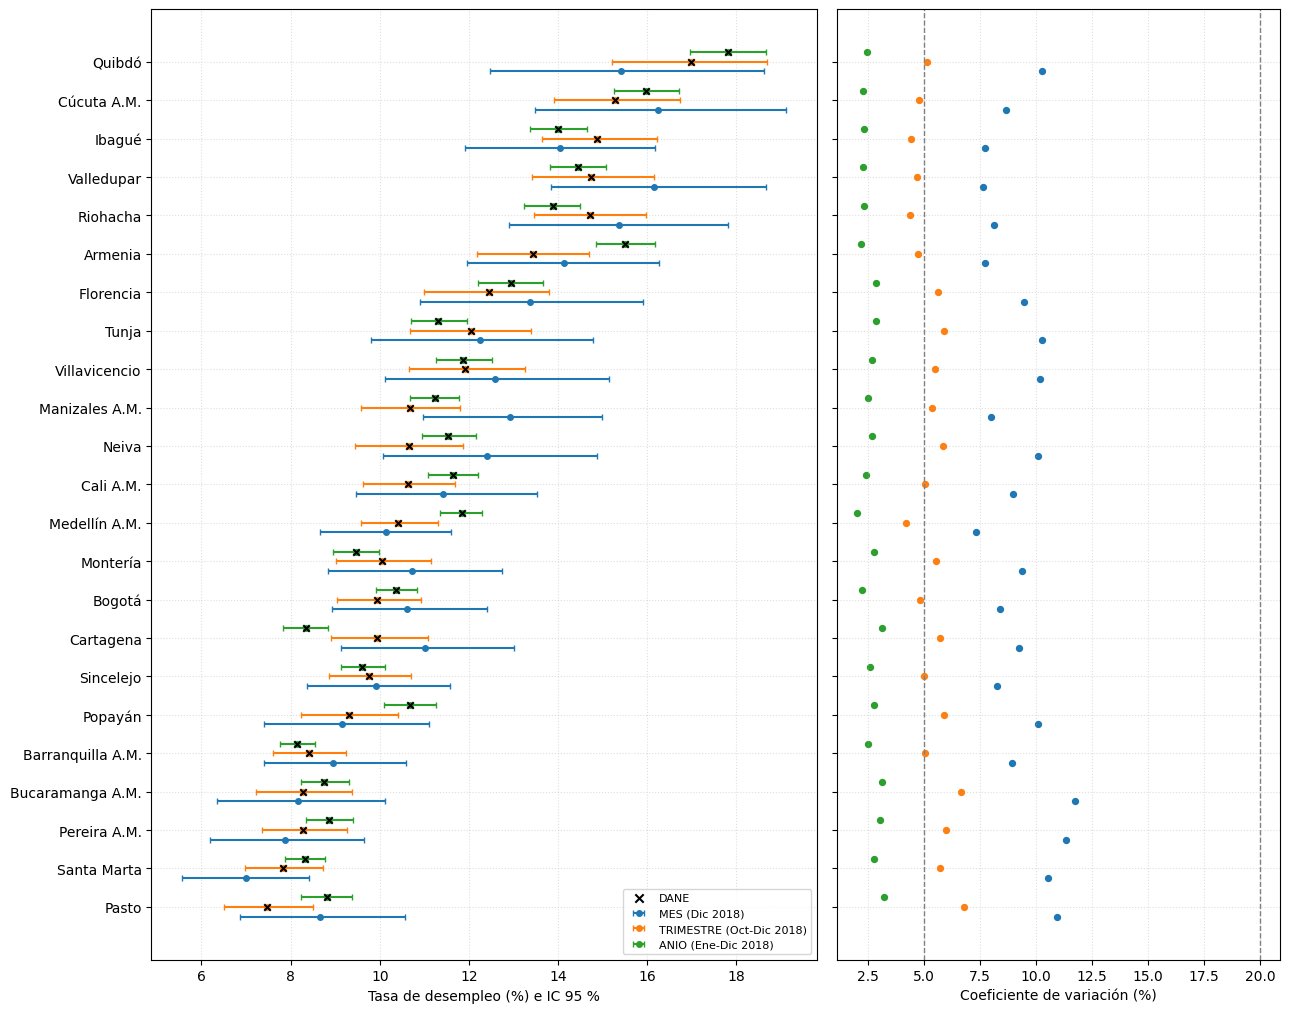
\includegraphics[width=\linewidth]{img/res_ventana_sensibilidad.png}
\caption{Tasa directa e intervalo bootstrap del 95~\% de cada dominio con las ventanas de un mes, un trimestre y un año, todas con cierre en diciembre de 2018. Fuente: tabla de sensibilidad de la ventana temporal.}
\label{fig:res_ventana}
\end{figure}

%--------------------------------------------------------------------------------------
\section{Construcción y agregación de las covariables}
\label{sec:res_covariables}

Las 18 covariables activas tienen dato en diciembre de 2018 para todos los municipios miembro de los dominios y para los 83 municipios objetivo; su geografía, período, unidad y denominador están en la Tabla~\ref{tab:covariables_datos}, y el catálogo con códigos y referencias, en el Apéndice~\ref{app:catalogo}. Las 6 variables de la literatura que no entraron se listan con su motivo en la Tabla~\ref{tab:res_excluidas} del Apéndice~\ref{app:resultados}: cuatro no tienen dato municipal para 2018, la pobreza monetaria no existe en los municipios objetivo y el índice de incidencia del conflicto armado se retiró.

La Tabla~\ref{tab:res_agregacion_am} del Apéndice~\ref{app:resultados} muestra cuánto cambian las covariables de los 7 dominios con área metropolitana si todas se agregan con la población de 15 años y más en lugar de su denominador propio (Ecuación~\ref{eq:agregacion}). En 14 de las 18 el cambio máximo es menor que 1~\%. Cambian mucho la densidad de población, que con la superficie como peso baja hasta 67.67~\% en Bucaramanga A.M., y las tres participaciones del valor agregado, que con el valor agregado como peso cambian hasta 43.94~\% en Cali A.M. En esas variables la regla elegida sí define el valor del dominio.

La tabla de municipios objetivo quedó con 83 filas: 41 del Cauca y 42 del Valle del Cauca. Se excluyó Popayán, que es un dominio por sí solo. Cali y Yumbo se conservaron con Cali A.M. como dominio de referencia.

%--------------------------------------------------------------------------------------
\section{Pre-filtrado de covariables}
\label{sec:res_prefiltrado}

La Tabla~\ref{tab:res_prefiltrado} muestra la cascada. La completitud retira dos de cada tres indicadores; la variabilidad, solo 12 más. El número de sobrevivientes cambia poco con los umbrales: con un CV mínimo entre 0.0001 y 0.01 y una proporción modal entre 0.80 y 0.95 quedan entre 493 y 499; solo con un CV mínimo de 0.05 baja a 475-478. Las 18 candidatas del catálogo pasaron los dos filtros. Entre los 497 sobrevivientes hay 19 grupos de indicadores prácticamente idénticos ($|r| \geq 0.999$), con 140 variables sobrantes, casi todos conteos de población por edad y sexo; se reportaron y no se usaron para decidir.

\begin{table}[!htbp]
\centering
\small
\caption{Cascada del pre-filtrado de los indicadores de TerriData en los 23 dominios.}
\label{tab:res_prefiltrado}
\begin{adjustbox}{max width=\linewidth}
\begin{tabular}{l l r r}
\toprule
Paso & Criterio & Indicadores & Retención (\%) \\
\midrule
Conjunto inicial & Indicadores en formato ancho & \num{1582} & 100.00 \\
Completitud & Sin faltantes en los 23 dominios & 509 & 32.17 \\
Variabilidad & CV $\geq 0.001$ y proporción modal $\leq 0.90$ & 497 & 31.42 \\
\bottomrule
\end{tabular}
\end{adjustbox}
\end{table}

%--------------------------------------------------------------------------------------
\section{Análisis descriptivo}
\label{sec:res_descriptivo}

La Figura~\ref{fig:res_respuesta} resume la tasa directa y su precisión. La tasa va de 8.15~\% en Barranquilla A.M. a 17.81~\% en Quibdó, con media 11.54~\% y mediana 11.31~\%; la asimetría es 0.67 y ningún dominio queda por fuera de la regla del diagrama de caja. El error estándar crece con la tasa (correlación de 0.86): los dominios con más desempleo son también los menos precisos. Quibdó, Cúcuta A.M. y Armenia tienen las tasas más altas; Barranquilla A.M., Santa Marta y Cartagena, las más bajas.

\begin{figure}[!htbp]
\centering
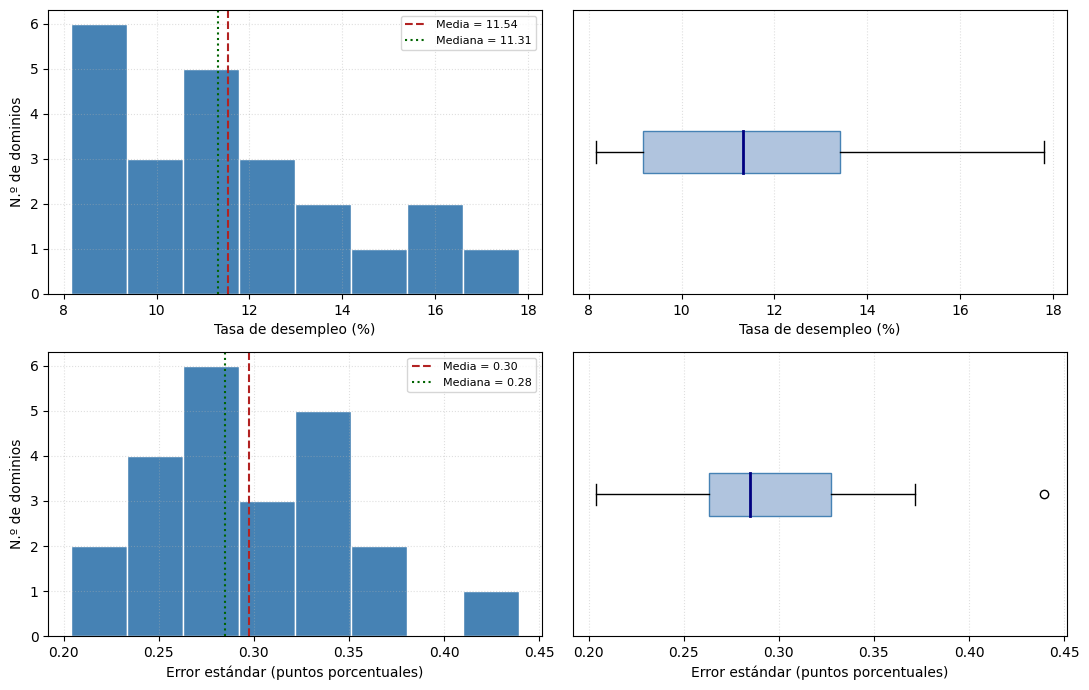
\includegraphics[width=\linewidth]{img/desc_respuesta_precision.png}
\caption{Distribución de la tasa directa, de su error estándar y de su CV en los 23 dominios, y relación entre la tasa y su error estándar. Fuente: tabla de estimación directa.}
\label{fig:res_respuesta}
\end{figure}

La Tabla~\ref{tab:res_bivariado} reúne la descripción bivariada de las 18 candidatas. Ninguna alcanza $|r| \geq 0.50$ con la tasa; diez quedan entre 0.30 y 0.50. En cinco la correlación de Pearson y la de Spearman difieren en más de 0.20, señal de que unos pocos dominios extremos sostienen la relación lineal: la tasa de homicidios, la cobertura de acueducto, el índice de pobreza multidimensional y los dos puntajes de las pruebas Saber 11. Dos candidatas tienen un signo contrario al esperado por el catálogo: la tasa de tránsito a la educación superior y el porcentaje de población urbana.

\begin{table}[!htbp]
\centering
\small
\caption{Asociación de cada candidata con la tasa directa en los 23 dominios. $r$: Pearson; $\rho_S$: Spearman; IC: intervalo de Fisher del 95~\% de $r$ (Ecuación~\ref{eq:ic_fisher}); Signo: esperado por el catálogo. Ordenadas por $|r|$.}
\label{tab:res_bivariado}
\begin{adjustbox}{max width=\linewidth}
\begin{tabular}{l c r r c}
\toprule
Covariable & Signo & $r$ & $\rho_S$ & IC de $r$ \\
\midrule
Tasa de homicidios & $+$ & 0.519 & 0.393 & [0.135, 0.767] \\
Cobertura de acueducto & $-$ & $-0.489$ & $-0.176$ & [$-0.750$, $-0.096$] \\
Cobertura neta en educación media & $-$ & $-0.476$ & $-0.513$ & [$-0.742$, $-0.079$] \\
Índice de pobreza multidimensional & $+$ & 0.441 & 0.184 & [0.035, 0.722] \\
Valor agregado de actividades primarias & $\pm$ & 0.432 & 0.499 & [0.024, 0.717] \\
Ingresos tributarios per cápita & $-$ & $-0.421$ & $-0.489$ & [$-0.710$, $-0.011$] \\
Cobertura neta en educación secundaria & $-$ & $-0.372$ & $-0.393$ & [$-0.680$, 0.047] \\
Valor agregado de actividades secundarias & $\pm$ & $-0.367$ & $-0.286$ & [$-0.677$, 0.053] \\
Valor agregado per cápita & $-$ & $-0.364$ & $-0.385$ & [$-0.675$, 0.056] \\
Tránsito a la educación superior & $-$ & 0.360 & 0.425 & [$-0.061$, 0.673] \\
Índice de desempeño fiscal & $-$ & $-0.315$ & $-0.406$ & [$-0.644$, 0.112] \\
Población joven de 14 a 28 años & $+$ & 0.309 & 0.211 & [$-0.118$, 0.640] \\
Saber 11, lectura crítica & $-$ & $-0.305$ & $-0.085$ & [$-0.637$, 0.122] \\
Densidad de población & $\pm$ & $-0.282$ & $-0.358$ & [$-0.622$, 0.147] \\
Saber 11, matemáticas & $-$ & $-0.269$ & $-0.068$ & [$-0.613$, 0.161] \\
Valor agregado de actividades terciarias & $\pm$ & 0.200 & 0.138 & [$-0.232$, 0.565] \\
Penetración de banda ancha & $-$ & $-0.121$ & $-0.078$ & [$-0.508$, 0.306] \\
Población urbana & $+$ & $-0.017$ & 0.052 & [$-0.426$, 0.398] \\
\bottomrule
\end{tabular}
\end{adjustbox}
\end{table}

En el plano multivariado, seis pares de candidatas tienen $|r| \geq 0.80$: los dos puntajes de Saber 11 (0.970), el valor agregado per cápita y los ingresos tributarios per cápita (0.931), las participaciones secundaria y terciaria del valor agregado ($-0.907$), la lectura crítica y el índice de pobreza multidimensional ($-0.850$), ese índice y la banda ancha ($-0.828$), y el desempeño fiscal y los ingresos tributarios (0.813). La estadística univariada de las candidatas, sus diagramas de caja, los diagramas de dispersión y la matriz de correlaciones están en el Apéndice~\ref{app:descriptivo}.

%--------------------------------------------------------------------------------------
\section{Selección de covariables}
\label{sec:res_seleccion}

La Tabla~\ref{tab:res_seleccion} muestra el recorrido de cada candidata por los cinco pasos. De las 18, tres tienen un valor $q$ de Benjamini-Hochberg menor o igual a 0.10 en el Fay-Herriot univariado, las tres con $q = 0.079$: la tasa de homicidios, la cobertura de acueducto y la cobertura neta en educación media. Con la cota de $\lfloor 23/10 \rfloor = 2$ covariables entraron las dos de mayor $|r_w|$: la tasa de homicidios ($r_w = 0.516$) y la cobertura de acueducto ($r_w = -0.486$). Su VIF es 1.98, por debajo de 5, y exigir el signo esperado no cambia el conjunto.

\begin{table}[!htbp]
\centering
\small
\caption{Ficha de decisión de la selección de covariables. $r_w$: correlación ponderada del Fay-Herriot univariado (Ecuación~\ref{eq:r_ponderada}); $q$: valor de Benjamini-Hochberg sobre 18 (Ecuación~\ref{eq:bh}); Robustez: D = depende de un dominio, E = estable; Soporte: proporción de los 83 municipios objetivo dentro del rango de los dominios. Ordenadas por $|r_w|$.}
\label{tab:res_seleccion}
\begin{adjustbox}{max width=\linewidth}
\begin{tabular}{l r r c r l}
\toprule
Covariable & $r_w$ & $q$ & Robustez & Soporte & Decisión \\
\midrule
Tasa de homicidios & 0.516 & 0.079 & D & 0.747 & Seleccionada \\
Cobertura de acueducto & $-0.486$ & 0.079 & D & 0.867 & Seleccionada \\
Cobertura neta en educación media & $-0.475$ & 0.079 & D & 0.518 & Elegible, fuera de la cota \\
Índice de pobreza multidimensional & 0.438 & 0.101 & D & 0.747 & Redundante (banda ancha) \\
Valor agregado de actividades primarias & 0.431 & 0.101 & E & 0.169 & No elegible \\
Ingresos tributarios per cápita & $-0.420$ & 0.101 & E & 0.590 & Redundante (valor agregado per cápita) \\
Cobertura neta en educación secundaria & $-0.372$ & 0.135 & D & 0.169 & No elegible \\
Valor agregado de actividades secundarias & $-0.365$ & 0.135 & D & 0.663 & Redundante (terciarias) \\
Valor agregado per cápita & $-0.362$ & 0.135 & E & 0.554 & No elegible \\
Tránsito a la educación superior & 0.361 & 0.135 & E & 0.169 & No elegible \\
Índice de desempeño fiscal & $-0.315$ & 0.202 & E & 0.506 & No elegible \\
Población joven de 14 a 28 años & 0.307 & 0.202 & D & 0.723 & No elegible \\
Saber 11, lectura crítica & $-0.302$ & 0.202 & D & 0.699 & Redundante (matemáticas) \\
Densidad de población & $-0.282$ & 0.228 & E & 0.771 & No elegible \\
Saber 11, matemáticas & $-0.266$ & 0.247 & D & 0.771 & No elegible \\
Valor agregado de actividades terciarias & 0.198 & 0.398 & D & 0.373 & No elegible \\
Penetración de banda ancha & $-0.120$ & 0.615 & D & 0.217 & No elegible \\
Población urbana & $-0.017$ & 0.938 & D & 0.265 & No elegible \\
\bottomrule
\end{tabular}
\end{adjustbox}
\end{table}

Los diagnósticos que no deciden dejan advertencias sobre el conjunto elegido. Doce de las 18 candidatas, incluidas las dos seleccionadas, dependen de un dominio según la regla de la Tabla~\ref{tab:met_seleccion}, y en 14 de esos casos el dominio influyente es Quibdó: sin él, la correlación ponderada de la tasa de homicidios baja 0.27 y la de la cobertura de acueducto, 0.39. La Figura~\ref{fig:res_robustez} sitúa cada candidata según su distancia de Cook máxima y ese cambio. En soporte, solo la cobertura de acueducto supera el 0.80; con la tasa de homicidios, 21 de los 83 municipios objetivo quedan fuera del rango de los dominios. La forma lineal resultó adecuada en las tres elegibles (ni el término cuadrático ni el logaritmo mejoran el AIC). El detalle de cada paso está en el Apéndice~\ref{app:seleccion}.

\begin{figure}[!htbp]
\centering
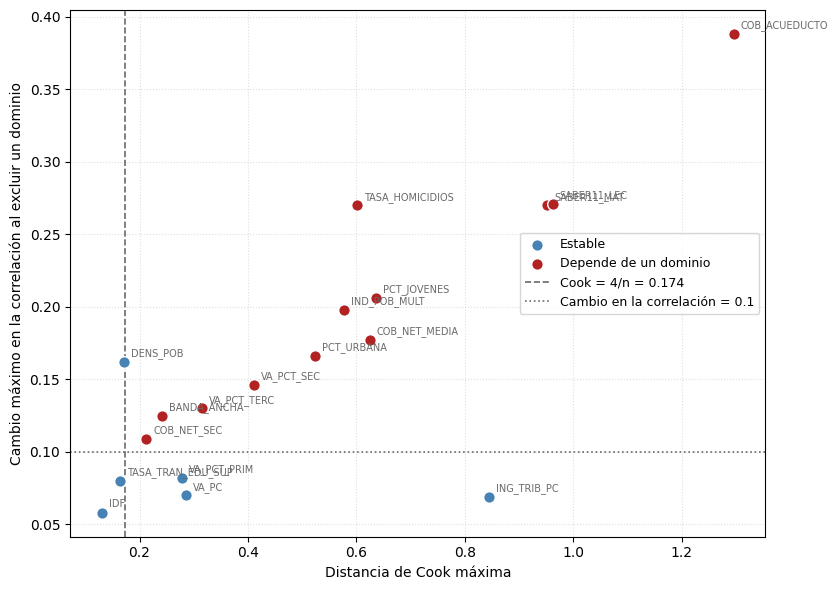
\includegraphics[width=0.85\linewidth]{img/eda_robustez.png}
\caption{Diagnóstico de robustez de las 18 candidatas: distancia de Cook máxima del Fay-Herriot univariado y cambio máximo de $r_w$ al retirar un dominio. Las líneas marcan $4/n = 0.174$ y el cambio de 0.10. Fuente: tabla de diagnósticos de covariables.}
\label{fig:res_robustez}
\end{figure}

%--------------------------------------------------------------------------------------
\section{Ajuste y selección del modelo Fay-Herriot clásico (benchmark)}
\label{sec:res_fh_clasico}

La Tabla~\ref{tab:res_especificaciones} compara las cuatro especificaciones. En EC1, con las dos covariables seleccionadas, ninguna es significativa ($p = 0.190$ y $p = 0.351$): comparten buena parte de la información, porque las dos dependen de Quibdó. Por eso EC1 no compite. Entre las tres que cumplen la regla, EC3 (tasa de homicidios) tiene el menor AIC, 108.904; EC2 (cobertura de acueducto) queda a 0.918 y es equivalente por la regla de $\Delta$AIC $\leq 2$. Como las dos tienen una covariable, la parsimonia no las separa y la elección la define el AIC. EC0 queda a 5.138 del mejor y no es equivalente. El AICc ordena igual. La RMSE de dejar un dominio fuera, que es descriptiva, también ordena a EC3 primero.

\begin{table}[!htbp]
\centering
\small
\caption{Especificaciones candidatas del modelo base Fay-Herriot clásico. $p$: valor $p$ máximo de las covariables; $\hat{\sigma}_u^2$ en puntos porcentuales al cuadrado; AIC y AICc con la verosimilitud ML (Ecuación~\ref{eq:aic}); RMSE: error de estimación de cada dominio retirado, con las covariables fijas (descriptiva). La especificación elegida está marcada con *.}
\label{tab:res_especificaciones}
\begin{adjustbox}{max width=\linewidth}
\begin{tabular}{l l r r r r r r r}
\toprule
 & Covariables & $p$ & $\hat{\sigma}_u^2$ & $R^2$ & AIC & $\Delta$AIC & AICc & RMSE \\
\midrule
EC3* & Homicidios & 0.006 & 5.529 & 0.269 & 108.904 & 0.000 & 110.167 & 2.52 \\
EC2 & Acueducto & 0.011 & 5.757 & 0.239 & 109.822 & 0.918 & 111.085 & 2.60 \\
EC1 & Homicidios y acueducto & 0.351 & 5.564 & 0.299 & 109.926 & 1.023 & 112.148 & 2.55 \\
EC0 & Solo intercepto & no aplica & 7.209 & 0.000 & 114.042 & 5.138 & 114.642 & 2.77 \\
\bottomrule
\end{tabular}
\end{adjustbox}
\end{table}

La Tabla~\ref{tab:res_coeficientes} muestra los coeficientes del benchmark. Cada 10 homicidios adicionales por cada 100,000 habitantes se asocian con 0.99 puntos porcentuales más de tasa de desempleo, condicional a la selección. El $R^2$ del componente sintético es 0.269: la tasa de homicidios deja sin explicar la mayor parte de la diferencia entre dominios. Frente al modelo de solo intercepto, $\hat{\sigma}_u^2$ baja de 7.209 a 5.529, es decir, un 23~\%.

\begin{table}[!htbp]
\centering
\small
\caption{Coeficientes del benchmark EC3, estimados por GLS (Ecuación~\ref{eq:gls}) con $\hat{\sigma}_u^2 = 5.529$ por REML. EE: error estándar. Los valores $p$ son descriptivos (Sección~\ref{sec:met_fh_clasico}).}
\label{tab:res_coeficientes}
\begin{tabular}{l r r r r}
\toprule
Parámetro & $\hat{\beta}$ & EE & $z$ & $p$ \\
\midrule
Intercepto & 9.191 & 0.979 & 9.388 & $<0.001$ \\
Tasa de homicidios (por 100,000 habitantes) & 0.099 & 0.036 & 2.761 & 0.006 \\
\bottomrule
\end{tabular}
\end{table}

Con varianzas de muestreo entre 0.04 y 0.19 frente a $\hat{\sigma}_u^2 = 5.529$, el peso de la estimación directa es alto en todos los dominios: $\hat{\gamma}_d$ va de 0.966 en Quibdó a 0.993 en Barranquilla A.M., con media 0.984. En consecuencia, el EBLUP casi coincide con la estimación directa (la mayor diferencia es $-0.10$ puntos porcentuales, en Cúcuta A.M.) y el ECM baja en promedio un 1.16~\% frente a $\psi_d$. Los 23 dominios siguen siendo confiables con el EBLUP (Figura~\ref{fig:res_cv}). La tabla de los 23 EBLUP con su ECM y su CV está en el Apéndice~\ref{app:dominios_modelo}.

\begin{figure}[!htbp]
\centering
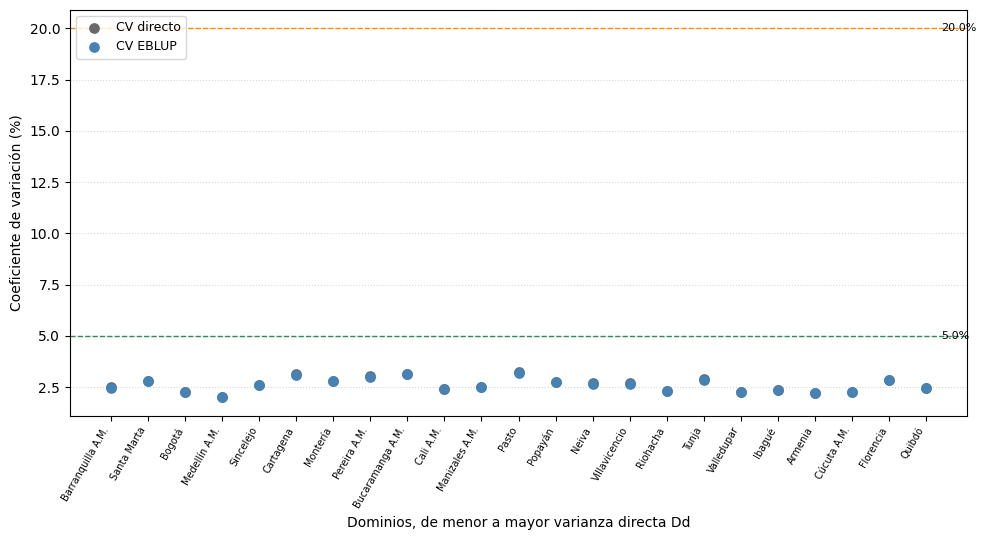
\includegraphics[width=0.85\linewidth]{img/fh_ganador_cv.png}
\caption{CV de la estimación directa y del EBLUP del benchmark por dominio, ordenados por la varianza de muestreo. Fuente: tabla de resultados del Fay-Herriot clásico.}
\label{fig:res_cv}
\end{figure}

%--------------------------------------------------------------------------------------
\section{Validación de supuestos y sensibilidad del benchmark}
\label{sec:res_supuestos}

La Tabla~\ref{tab:res_diagnosticos} reúne los diagnósticos del benchmark con el formato de la nota metodológica del DANE \cite{DANE_SAE_2025}. Los diagnósticos no muestran evidencia fuerte contra la aproximación normal en el benchmark, dentro de la limitada potencia disponible con 23 áreas. La media de los residuos es cercana a cero por construcción y no informa sobre sesgo. Los residuos tampoco muestran dependencia espacial con ninguna de las cuatro matrices (Sección~\ref{sec:res_espacial}). Los histogramas y gráficos de contracción de las cuatro especificaciones están en el Apéndice~\ref{app:especificaciones}.

\begin{table}[!htbp]
\centering
\small
\caption{Diagnósticos del benchmark EC3 sobre los residuos estandarizados (Ecuación~\ref{eq:residuos}).}
\label{tab:res_diagnosticos}
\begin{tabularx}{\linewidth}{>{\raggedright\arraybackslash}p{2.8cm} >{\raggedright\arraybackslash}p{3.9cm} >{\raggedright\arraybackslash}p{2.6cm} >{\raggedright\arraybackslash}X}
\toprule
Supuesto & Medida & Valor & Lectura \\
\midrule
Normalidad & Shapiro-Wilk (Ecuación~\ref{eq:shapiro}) & $W = 0.954$; $p = 0.357$ & Sin evidencia fuerte en contra, con baja potencia \\
Media cero & Media de los residuos & 0.002 & Cercana a cero por construcción del GLS \\
Varianza & Desviación estándar & 0.977 & Cercana a 1: $\psi_d$ y $\hat{\sigma}_u^2$ son compatibles con la dispersión observada \\
Independencia espacial & I de Moran, 3 vecinos (Ecuación~\ref{eq:moran}) & $I = 0.093$; $p = 0.333$ & Sin autocorrelación detectable \\
Influencia & Cook máxima (Ecuación~\ref{eq:cook}) & 0.601 (Quibdó) & Quibdó y Cali A.M. superan $4/n = 0.174$ \\
\bottomrule
\end{tabularx}
\end{table}

La Tabla~\ref{tab:res_estabilidad} resume la estabilidad del coeficiente de la tasa de homicidios. Al retirar un dominio, $\hat{\beta}_1$ queda entre 0.061 (sin Quibdó) y 0.125 (sin Cali A.M.). Sin Quibdó el cambio es de $-38.2$~\%, equivale a 1.05 errores estándar, supera el umbral de 1 y el coeficiente deja de ser significativo ($p = 0.256$); es el único de los 23 reajustes que cruza el umbral de significancia y ninguno cambia el signo. En el bootstrap de dominios el intervalo del 95~\% va de 0.011 a 0.191, el signo se conserva en el 98.6~\% de las réplicas y la significancia, en el 70.4~\%. La Figura~\ref{fig:res_loao} muestra el cambio estandarizado por dominio.

\begin{table}[!htbp]
\centering
\small
\caption{Estabilidad del coeficiente de la tasa de homicidios: 23 reajustes dejando un dominio fuera (reestimando $\hat{\sigma}_u^2$) y \num{1000} réplicas bootstrap de dominios. Cambio en EE: Ecuación~\ref{eq:dfbeta}.}
\label{tab:res_estabilidad}
\begin{tabularx}{\linewidth}{>{\raggedright\arraybackslash}X >{\raggedright\arraybackslash}p{6.4cm}}
\toprule
Medida & Resultado \\
\midrule
$\hat{\beta}_1$ con los 23 dominios & 0.099 (EE 0.036) \\
Mínimo y máximo al retirar un dominio & 0.061 (sin Quibdó) y 0.125 (sin Cali A.M.) \\
Cambio máximo & $-38.2$~\% $= -1.05$ EE (Quibdó); siguientes: Cali A.M. ($+0.71$ EE) y Tunja ($+0.25$ EE) \\
Cambios de signo y de significancia & 0 de 23 y 1 de 23 (Quibdó, $p = 0.256$) \\
Bootstrap: intervalo del 95~\% & [0.011, 0.191] \\
Bootstrap: mismo signo y $p < 0.05$ & 98.6~\% y 70.4~\% de las réplicas \\
Mayor cambio de un EBLUP de los otros dominios & 0.05 puntos porcentuales \\
Mayor cambio de una estimación municipal & $-7.65$ puntos porcentuales (Corinto, sin Quibdó) \\
Cambio máximo de $\hat{\sigma}_u^2$ & 11~\% \\
\bottomrule
\end{tabularx}
\end{table}

\begin{figure}[!htbp]
\centering
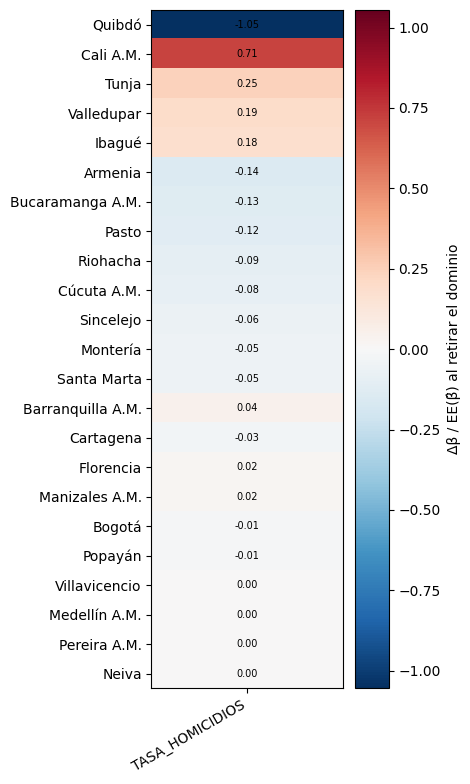
\includegraphics[width=0.85\linewidth]{img/fh_loao_influencia.png}
\caption{Cambio de cada coeficiente del benchmark, en errores estándar, al retirar cada dominio. Fuente: tabla de influencia dejar-un-dominio-fuera del Fay-Herriot clásico.}
\label{fig:res_loao}
\end{figure}

Los EBLUP de los dominios casi no se mueven al retirar un dominio, porque cada uno se apoya en su propia estimación directa. Las estimaciones municipales sí: retirar Quibdó cambia más de 0.5 puntos porcentuales la estimación de 51 municipios y retirar Cali A.M., la de 45. La influencia de un solo dominio se transmite a los municipios a través del coeficiente.

La Tabla~\ref{tab:res_varianza} resume la sensibilidad a la varianza de muestreo. Las varianzas alternativas son parecidas a la base: la de Taylor tiene razón mediana 1.000 con la del bootstrap, y la del bootstrap por personas es menor (razón 1.104, entre 0.939 y 1.173), como se espera al ignorar la correlación dentro de la vivienda. Las dos GVF se ajustan bien ($R^2$ de 0.970 y 0.976; Figura~\ref{fig:app_gvf}). En los nueve escenarios el benchmark sigue siendo EC3, el coeficiente conserva signo y significancia, y el EBLUP cambia como máximo 0.20 puntos porcentuales. Solo al triplicar $\psi_d$ cuatro dominios pasan de confiables a aceptables. La razón $\hat{\sigma}_u^2/\bar{\psi}$, entre 19.5 y 184.2, explica por qué el modelo es poco sensible a $\psi_d$: con una varianza entre dominios tan grande frente a la de muestreo, $\hat{\gamma}_d$ se mantiene cerca de 1 en todos los escenarios \cite[p.~143]{Benedetti2024}.

\begin{table}[!htbp]
\centering
\small
\caption{Escenarios de la varianza de muestreo. $\bar{\psi}$: media de $\psi_d$; $\Delta$EBLUP y $\Delta$sintético: cambio máximo frente al escenario base, en puntos porcentuales; Conf.: dominios confiables con el EBLUP. En todos los escenarios el benchmark es EC3.}
\label{tab:res_varianza}
\begin{adjustbox}{max width=\linewidth}
\begin{tabular}{l r r r r r r}
\toprule
Escenario & $\hat{\sigma}_u^2$ & $\hat{\sigma}_u^2/\bar{\psi}$ & $\min \hat{\gamma}_d$ & $\Delta$EBLUP & $\Delta$sintético & Conf. \\
\midrule
Base (bootstrap de viviendas) & 5.529 & 60.7 & 0.966 & 0.00 & 0.00 & 23 \\
Taylor & 5.527 & 60.4 & 0.966 & 0.00 & 0.00 & 23 \\
GVF A & 5.524 & 60.6 & 0.967 & 0.01 & 0.00 & 23 \\
$\psi_d \times 1/3$ & 5.595 & 184.2 & 0.989 & 0.07 & 0.04 & 23 \\
$\psi_d \times 1/2$ & 5.578 & 122.4 & 0.983 & 0.05 & 0.03 & 23 \\
$\psi_d \times 2/3$ & 5.562 & 91.6 & 0.977 & 0.03 & 0.02 & 23 \\
$\psi_d \times 3/2$ & 5.480 & 40.1 & 0.950 & 0.05 & 0.03 & 23 \\
$\psi_d \times 2$ & 5.430 & 29.8 & 0.934 & 0.10 & 0.06 & 23 \\
$\psi_d \times 3$ & 5.332 & 19.5 & 0.902 & 0.20 & 0.13 & 19 \\
\bottomrule
\end{tabular}
\end{adjustbox}
\end{table}

%--------------------------------------------------------------------------------------
\section{Validación predictiva dejar-un-dominio-fuera}
\label{sec:res_validacion}

Con los 23 dominios, la selección repetida reproduce el conjunto de la etapa 9 y el benchmark de la etapa 10, como exige la verificación de la Tabla~\ref{tab:met_validacion}. La Tabla~\ref{tab:res_validacion} presenta las métricas de los dos ejercicios y del modelo de solo intercepto.

\begin{table}[!htbp]
\centering
\small
\caption{Validación predictiva dejar-un-dominio-fuera: error de la estimación sintética de cada dominio retirado frente a su estimación directa (Ecuación~\ref{eq:metricas_val}). Errores en puntos porcentuales; cobertura del intervalo nominal del 95~\%; habilidad frente al modelo de solo intercepto.}
\label{tab:res_validacion}
\begin{adjustbox}{max width=\linewidth}
\begin{tabular}{l r r r}
\toprule
Métrica & Covariables fijas & Procedimiento completo & Solo intercepto \\
\midrule
RMSE & 2.52 & 3.43 & 2.77 \\
MAE & 2.13 & 2.91 & 2.23 \\
Sesgo medio & $-0.07$ & $-0.41$ & $-0.01$ \\
RMSE corregida por ruido & 2.51 & 3.42 & 2.76 \\
$Z_{\text{pred}}$: media y desviación & $-0.02$; 1.05 & $-0.17$; 1.44 & $-0.02$; 1.07 \\
Cobertura (\%) & 100.00 & 86.96 & 95.65 \\
Habilidad frente al modelo nulo & 0.17 & $-0.54$ & no aplica \\
\bottomrule
\end{tabular}
\end{adjustbox}
\end{table}

Con las covariables fijas, la tasa de homicidios mejora la RMSE del modelo nulo en un 17~\% (2.52 frente a 2.77). Ese ejercicio es optimista, porque la covariable se eligió viendo a todos los dominios. Cuando la selección se repite en cada iteración, la RMSE sube a 3.43, por encima de la del modelo de solo intercepto, y la habilidad pasa a $-0.54$: el procedimiento completo estima peor que el promedio de los dominios. La diferencia entre 2.52 y 3.43 es el costo de seleccionar y estimar con los mismos 23 dominios. Frente al error dentro de muestra (2.27), la validación con covariables fijas lo infla 1.11 veces y el procedimiento completo, 1.52.

La inestabilidad de la selección explica ese costo. El procedimiento reproduce el benchmark en 14 de las 23 iteraciones y produce 6 conjuntos distintos; la tasa de homicidios entra al benchmark en el 69.57~\% de las iteraciones y la cobertura de acueducto, en el 8.70~\% (Tabla~\ref{tab:res_frecuencia} del Apéndice~\ref{app:resultados}). Sin Florencia, Quibdó, Riohacha o Pasto no queda ninguna covariable elegible y se usa solo el intercepto; sin Bogotá entra el ingreso tributario per cápita, sin Neiva el valor agregado primario y sin Armenia la cobertura neta en media. En tres dominios el error estandarizado supera 1.96 en valor absoluto: Armenia ($-3.17$), Quibdó ($-2.66$) y Cúcuta A.M. ($-2.15$). Los errores por dominio y la figura de los dos ejercicios están en el Apéndice~\ref{app:validacion}.

%--------------------------------------------------------------------------------------
\section{Modelo Fay-Herriot espacial y comparación con el benchmark}
\label{sec:res_espacial}

Los 23 dominios están lejos entre sí: el vecino más cercano de cada uno está entre 30 y 158 km, con mediana de 106 km, y 12 lo tienen a más de 100 km. Los municipios objetivo están más cerca de algún dominio: la distancia mediana al más cercano es 46.3 km en el Cauca y 44.6 km en el Valle del Cauca. La Tabla~\ref{tab:res_espacial} presenta el ajuste del benchmark y de las especificaciones espaciales con la tasa de homicidios fija.

\begin{table}[!htbp]
\centering
\small
\caption{Ajuste del benchmark y de las especificaciones espaciales (misma respuesta, mismos $\psi_d$, mismos 23 dominios, tasa de homicidios fija). $\Delta$AIC = AIC clásico $-$ AIC espacial (positivo favorece al espacial); LRT de $\rho = 0$ (Ecuación~\ref{eq:lrt}); RMSE de la validación dejar-un-dominio-fuera del predictor espacial (estructura completa) o de la estimación sintética (muestra). Las ocho especificaciones están en el Apéndice~\ref{app:espacial}.}
\label{tab:res_espacial}
\begin{adjustbox}{max width=\linewidth}
\begin{tabular}{l r r r r r r r}
\toprule
Especificación & $\hat{\sigma}_u^2$ & $\hat{\rho}$ & AIC & $\Delta$AIC & LRT & $p$ & RMSE \\
\midrule
Clásico (benchmark) & 5.529 & no aplica & 108.904 & no aplica & no aplica & no aplica & 2.52 \\
3 vecinos, muestra & 5.383 & 0.234 & 110.572 & $-1.669$ & 0.331 & 0.565 & 2.53 \\
3 vecinos, completa (referencia) & 4.825 & 0.372 & 109.403 & $-0.500$ & 1.500 & 0.221 & 2.35 \\
Otras seis: mínimo & 5.101 & 0.187 & 110.105 & $-1.998$ & 0.003 & 0.371 & 2.48 \\
Otras seis: máximo & 5.631 & 0.891 & 110.901 & $-1.201$ & 0.799 & 0.960 & 2.86 \\
\bottomrule
\end{tabular}
\end{adjustbox}
\end{table}

Ninguna de las ocho especificaciones espaciales cumple el criterio. En la estructura «muestra» del escenario de referencia, $\hat{\rho} = 0.234$ y $p(\text{LRT}) = 0.565$; en todas, $p \geq 0.221$, y el AIC del espacial es mayor que el del clásico, lo que corresponde a $\text{LRT} < 2$. El perfil de verosimilitud del escenario de referencia es plano: su intervalo del 95~\% para $\rho$ va de $-0.15$ a 0.75 (Figura~\ref{fig:app_perfil_rho}). Los $\hat{\rho}$ de la estructura «completa» llegan hasta 0.891 con distancia inversa de potencia 1, pero cambian según los municipios que se incluyen como nodos (0.398 con solo los del Valle y 0.262 con solo los del Cauca, con 3 vecinos), por lo que no se interpretan. Ubicar el nodo de cada área metropolitana en la media de sus municipios cambia $\hat{\rho}$ como máximo en 0.131 y ningún $p$ baja de 0.354. Con este resultado, el modelo recomendado es el benchmark clásico y el espacial queda como análisis de sensibilidad.

La Tabla~\ref{tab:res_moran} compara el I de Moran de los residuos estandarizados del clásico con el de los residuos del SEBLUP. Ningún índice es significativo; los del clásico van de $-0.023$ a 0.093 y los del espacial, de $-0.115$ a $-0.038$. La tasa directa tampoco muestra autocorrelación (I entre $-0.028$ y 0.003). La Figura~\ref{fig:res_mapa_residuos} muestra los residuos sobre el mapa: los dominios con residuos del mismo signo no se agrupan, y los mayores (Cúcuta A.M. y Valledupar, positivos; Barranquilla A.M. y Cartagena, negativos) quedan en regiones distintas.

\begin{table}[!htbp]
\centering
\small
\caption{I de Moran de los residuos estandarizados del clásico y de los residuos del SEBLUP, con la misma matriz estandarizada por filas en cada escenario; $p$ por \num{9999} permutaciones. $E[I] = -0.045$.}
\label{tab:res_moran}
\begin{tabular}{l r r r r r r}
\toprule
 & \multicolumn{2}{c}{Clásico} & \multicolumn{2}{c}{SEBLUP muestra} & \multicolumn{2}{c}{SEBLUP completa} \\
\cmidrule(lr){2-3}\cmidrule(lr){4-5}\cmidrule(lr){6-7}
Matriz & $I$ & $p$ & $I$ & $p$ & $I$ & $p$ \\
\midrule
3 vecinos & 0.093 & 0.333 & $-0.043$ & 0.984 & $-0.110$ & 0.658 \\
5 vecinos & 0.005 & 0.605 & $-0.038$ & 0.938 & $-0.038$ & 0.936 \\
Inversa, potencia 1 & $-0.023$ & 0.650 & $-0.055$ & 0.848 & $-0.057$ & 0.819 \\
Inversa, potencia 2 & 0.013 & 0.599 & $-0.069$ & 0.830 & $-0.115$ & 0.522 \\
\bottomrule
\end{tabular}
\end{table}

\begin{figure}[!htbp]
\centering
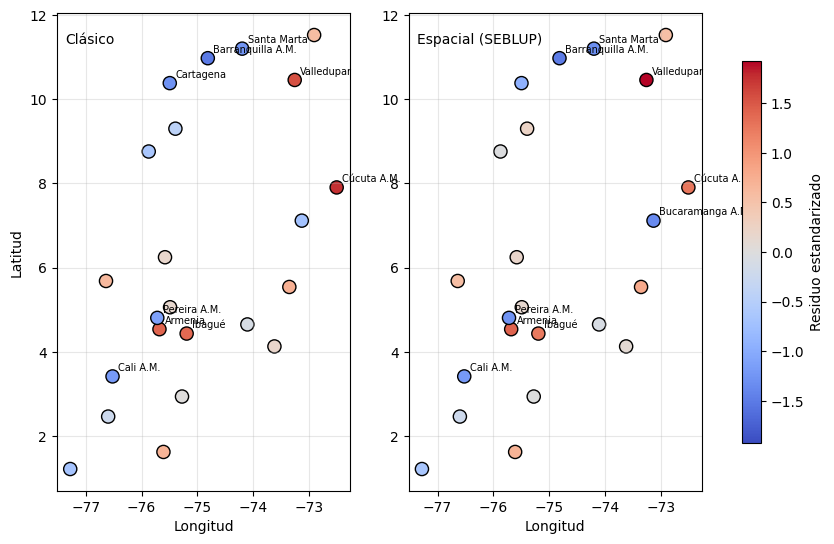
\includegraphics[width=0.9\linewidth]{img/fhe_mapa_residuos.png}
\caption{Residuos estandarizados de los 23 dominios en el clásico y en el SEBLUP del escenario de referencia (3 vecinos, estructura completa), ubicados en la cabecera de la capital. Fuente: tablas de Moran y de comparación del modelo espacial.}
\label{fig:res_mapa_residuos}
\end{figure}

La Tabla~\ref{tab:res_comparacion} completa la comparación controlada con la incertidumbre, las estimaciones y los coeficientes. El ECM y el CV del SEBLUP de los 23 dominios, su peso $\hat{\gamma}^{S}_d$ y las diferencias en los dominios no los guardaba el procesamiento; se calcularon reajustando el SEBLUP del escenario de referencia con la misma clase del código, que reproduce $\hat{\rho} = 0.372$ y $\hat{\sigma}_u^2 = 4.825$ con 500 réplicas válidas de 500 (Ecuaciones~\ref{eq:seblup} y~\ref{eq:gamma_esp}).

\begin{table}[!htbp]
\centering
\small
\caption{Comparación controlada entre el benchmark (EBLUP y estimación sintética) y el escenario espacial de referencia (SEBLUP y predictor espacial). Diferencias = espacial $-$ clásico, en puntos porcentuales; clases de CV con los umbrales de 5 y 20~\%. Fuente: tablas del modelo; dominios: cálculo propio sobre esas tablas.}
\label{tab:res_comparacion}
\begin{tabularx}{\linewidth}{>{\raggedright\arraybackslash}X >{\raggedleft\arraybackslash}p{3.3cm} >{\raggedleft\arraybackslash}p{3.3cm}}
\toprule
Elemento & 23 dominios & 83 municipios \\
\midrule
CV mediano: clásico y espacial (\%) & 2.60 y 2.60 & 19.49 y 19.87 \\
ECM medio: clásico y espacial & 0.090 y 0.091 & no aplica \\
Peso de la directa: $\hat{\gamma}_d$ y $\hat{\gamma}^S_d$ (medias) & 0.984 y 0.982 & no aplica \\
Diferencia media & 0.00 & $-0.03$ \\
Diferencia absoluta media & 0.01 & 0.22 \\
Diferencia absoluta máxima & 0.02 & 2.79 (Cali) \\
Casos con diferencia absoluta mayor que 0.5 & 0 & 8 \\
Correlación de Pearson y de Spearman & 1.000 y 1.000 & 0.992 y 0.987 \\
Cambios de clase de confiabilidad & 0 & 8 (7 de no confiable a aceptable) \\
Coeficiente de la tasa de homicidios (EE) & \multicolumn{2}{c}{clásico 0.099 (0.036); espacial 0.102 (0.035); diferencia 0.07 EE} \\
\bottomrule
\end{tabularx}
\end{table}

En los dominios, las dos estimaciones son prácticamente iguales: la mayor diferencia es 0.02 puntos porcentuales y la precisión no cambia. En los municipios, la estimación espacial agrega a la sintética el efecto que el modelo infiere de los dominios cercanos; ese efecto es pequeño en casi todos (Figura~\ref{fig:res_espacial_estimaciones}). Las dos diferencias grandes son Cali y Yumbo ($-2.79$ y $-2.72$ puntos porcentuales), que reciben el efecto estimado de Cali A.M. y no uno propio. Les siguen Caicedonia (0.79), Jamundí ($-0.74$), Ulloa (0.66), El Águila (0.64), Alcalá (0.59) y Candelaria ($-0.55$), todos a menos de 40 km de un dominio. El coeficiente de la tasa de homicidios cambia menos de 0.13 errores estándar del clásico en las ocho especificaciones.

\begin{figure}[!htbp]
\centering
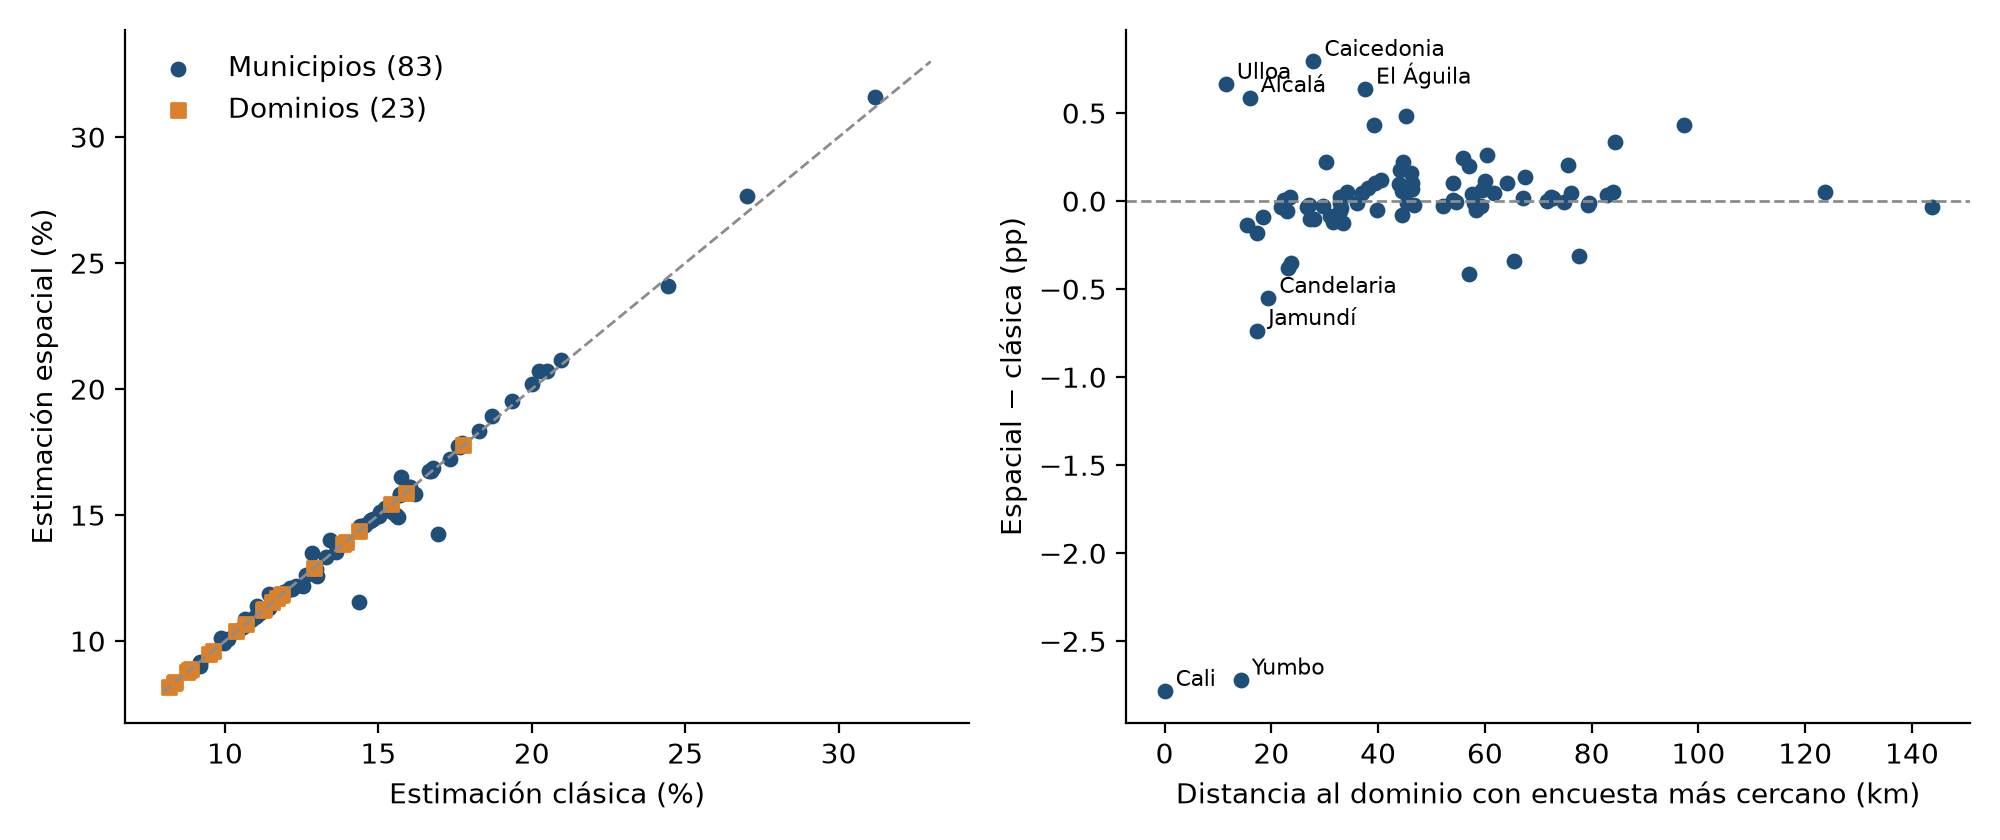
\includegraphics[width=\linewidth]{img/res_espacial_estimaciones.png}
\caption{Izquierda: estimación clásica frente a espacial en los 23 dominios (EBLUP y SEBLUP) y en los 83 municipios (sintética y espacial). Derecha: diferencia en los municipios según la distancia al dominio con encuesta más cercano; se nombran los que difieren más de 0.5 puntos porcentuales. Fuente: tabla de estimaciones de los municipios objetivo del modelo espacial y cálculo propio de los dominios.}
\label{fig:res_espacial_estimaciones}
\end{figure}

En la validación dejar-un-dominio-fuera con las covariables fijas (Tabla~\ref{tab:res_validacion_espacial} del Apéndice~\ref{app:resultados}), el predictor espacial del escenario de referencia tiene la menor RMSE: 2.35, frente a 2.48 de la estimación sintética espacial, 2.52 de la sintética clásica y 2.77 del modelo de solo intercepto, con habilidad de 0.28. La ventaja no se repite en los otros escenarios: con 5 vecinos sube a 2.59 y con distancia inversa a 2.60 y 2.86, este último con habilidad negativa. Con 23 dominios y covariables fijas, estas diferencias se leen como orden de magnitud y no cambian la conclusión del LRT.

%--------------------------------------------------------------------------------------
\section{Estimación en los municipios sin cobertura muestral}
\label{sec:res_sin_muestra}

La Figura~\ref{fig:res_rangos} compara la tasa de homicidios de los municipios objetivo con el rango de los dominios, que va de 4.06 (Tunja) a 71.96 (Quibdó) homicidios por cada 100,000 habitantes. En los municipios va de 0 a 221.47, con mediana 42.67. Tres municipios quedan por debajo del rango (Ginebra, Puracé y Silvia, sin homicidios en 2018) y 18 por encima, de modo que 21 de los 83 son extrapolación (Ecuación~\ref{eq:hnew}). Con una sola covariable no puede haber combinaciones atípicas: el estado de los otros 62 es «dentro del rango».

\begin{figure}[!htbp]
\centering
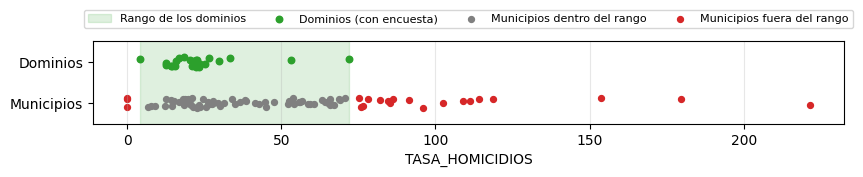
\includegraphics[width=\linewidth]{img/fh_rangos_covariables.png}
\caption{Tasa de homicidios de los 23 dominios y de los 83 municipios objetivo; la franja es el rango de los dominios. Fuente: tabla de rangos de covariables del Fay-Herriot clásico.}
\label{fig:res_rangos}
\end{figure}

La Tabla~\ref{tab:res_extrapolacion} resume las estimaciones sintéticas según su estado. En los 21 municipios que extrapolan, la parte de la estimación que viene de salirse del rango tiene mediana de 1.4 puntos porcentuales y máximo de 14.84, en Corinto, cuya estimación de 31.17~\% sería 16.33~\% con la tasa de homicidios recortada al máximo de los dominios. Diez municipios tienen una estimación mayor que 17.81~\%, la directa más alta de los dominios. Al retirar un dominio a la vez, la estimación de los que extrapolan se mueve en una franja mediana de 4.30 puntos porcentuales, frente a 0.79 en los que están dentro del rango (Figura~\ref{fig:app_sensibilidad_extrapolacion}).

\begin{table}[!htbp]
\centering
\small
\caption{Estimación sintética del benchmark en los 83 municipios, antes del benchmarking, según el estado de extrapolación. Tasas y RMSE en puntos porcentuales; CV en \%. Aporte: parte de la estimación que viene de salirse del rango.}
\label{tab:res_extrapolacion}
\begin{adjustbox}{max width=\linewidth}
\begin{tabular}{l r r r r r r}
\toprule
Estado y clase de CV & Municipios & Tasa media & Tasa máxima & CV medio & RMSE medio & Aporte medio \\
\midrule
Dentro del rango, aceptable & 33 & 14.36 & 16.19 & 18.48 & 2.65 & 0.00 \\
Dentro del rango, no confiable & 29 & 11.13 & 11.96 & 21.79 & 2.42 & 0.00 \\
Fuera del rango, aceptable & 15 & 18.36 & 20.96 & 18.85 & 3.47 & 2.03 \\
Fuera del rango, no confiable & 6 & 18.37 & 31.17 & 25.22 & 4.42 & 5.81 \\
\bottomrule
\end{tabular}
\end{adjustbox}
\end{table}

Ningún municipio queda confiable: el CV de la estimación sintética va de 18.07~\% a 27.71~\%, porque su ECM incluye $\hat{\sigma}_u^2 = 5.529$ completo (Ecuación~\ref{eq:var_sintetica}). El CV no distingue a los que extrapolan: su CV medio es 20.7~\% frente a 20.0~\% de los que no, aunque su RMSE medio es 1.5 veces mayor (3.74 frente a 2.54), porque la tasa estimada también sube y el cociente casi no cambia. Los CV más altos corresponden a las tasas más bajas, no a las estimaciones más dudosas: Ginebra, Puracé y Silvia, con tasa de 9.19~\%, igual al intercepto, tienen CV de 27.71~\%. Por eso la calidad reportada agrega la mención «condicional al modelo» a todos los municipios y «extrapolado (fuera del rango)» a los 21 que extrapolan. Las estimaciones de cada municipio con ambos modelos están en el Apéndice~\ref{app:municipios}.

%--------------------------------------------------------------------------------------
\section{Benchmarking y consolidación de las estimaciones}
\label{sec:res_benchmarking}

La Tabla~\ref{tab:res_benchmarking} presenta los dos niveles del benchmarking. En el nivel 1, el agregado de los 23 EBLUP ponderado por la PEA expandida es 10.8368~\% y la referencia es 10.8340~\%; el factor $\lambda_1 = 0.9997$ baja cada EBLUP entre 0.002 y 0.005 puntos porcentuales y no cambia ninguna clase. En el nivel 2, Cali y Yumbo, ponderados por su población de 15 años y más, suman 14.47~\%, mientras que el EBLUP ajustado de Cali A.M. es 11.69~\%: el factor $\lambda_D = 0.808$ los baja casi un 20~\%. La diferencia no viene de la forma de agregar las covariables: la brecha entre $\bar{\mathbf{x}}_D^\top\hat{\boldsymbol{\beta}}$ y el promedio ponderado de los sintéticos municipales es $-0.004$ puntos porcentuales. Viene de que Cali A.M. tiene una tasa de homicidios alta (el sintético del dominio es 14.48~\%) y una tasa directa mucho menor que la que anticipa esa covariable.

\begin{table}[!htbp]
\centering
\small
\caption{Benchmarking en dos niveles (Ecuaciones~\ref{eq:benchmarking} y~\ref{eq:rmse_bm}). Tasas en \%; CV en \% antes y después del ajuste.}
\label{tab:res_benchmarking}
\begin{tabularx}{\linewidth}{>{\raggedright\arraybackslash}X r r r r}
\toprule
Nivel y unidad & Antes & Referencia o después & $\lambda$ & CV antes y después \\
\midrule
Nivel 1: agregado de los 23 dominios & 10.84 & 10.83 & 0.9997 & sin cambio de clase \\
Nivel 2: agregado de Cali y Yumbo & 14.47 & 11.69 & 0.8077 & no aplica \\
\quad Cali & 14.36 & 11.60 & 0.8077 & 18.20 y 29.96 \\
\quad Yumbo & 16.96 & 13.70 & 0.8077 & 18.32 y 30.03 \\
\bottomrule
\end{tabularx}
\end{table}

Todas las verificaciones de la etapa pasaron: después del ajuste, el agregado reproduce la referencia con diferencias del orden de $10^{-15}$, las razones entre estimaciones se conservan, las tasas quedan en $[0, 100]$ y la comprobación sobre la tabla final redondeada también se cumple. El factor del nivel 2 supera el aviso de $|\lambda - 1| > 0.20$ por muy poco (0.192) y no lo activa, pero su efecto en la incertidumbre es grande: el sesgo $(\lambda - 1)\hat{\theta}$ del ajuste entra en la RMSE de la Ecuación~\ref{eq:rmse_bm} y el CV de Cali y Yumbo pasa de cerca de 18~\% a 30~\%, de modo que ambos quedan como no confiables.

La tabla final tiene 106 filas: los 23 dominios con el EBLUP ajustado, todos confiables (CV entre 2.01~\% y 3.20~\%), y los 83 municipios. La Tabla~\ref{tab:res_calidad} cuenta la calidad reportada de los municipios. En el Valle del Cauca la mitad de los municipios queda como aceptable dentro del rango (21 de 42); en el Cauca, 11 de 41. Frente a la Tabla~\ref{tab:res_extrapolacion}, Cali pasa de aceptable a no confiable y Yumbo, de aceptable extrapolado a no confiable extrapolado.

\begin{table}[!htbp]
\centering
\small
\caption{Calidad reportada de los 83 municipios en la tabla final, tras el benchmarking.}
\label{tab:res_calidad}
\begin{tabular}{l r r r}
\toprule
Calidad reportada & Cauca & Valle del Cauca & Total \\
\midrule
Aceptable, condicional al modelo & 11 & 21 & 32 \\
No confiable, condicional al modelo & 17 & 13 & 30 \\
Aceptable, condicional al modelo, extrapolado & 9 & 5 & 14 \\
No confiable, condicional al modelo, extrapolado & 4 & 3 & 7 \\
\midrule
Total & 41 & 42 & 83 \\
\bottomrule
\end{tabular}
\end{table}

%--------------------------------------------------------------------------------------
\section{Distribución y patrones espaciales de las estimaciones}
\label{sec:res_patrones}

La Figura~\ref{fig:res_mapa_municipios} muestra las 83 estimaciones finales, su calidad reportada y el efecto espacial. La tasa estimada va de 9.19~\% a 31.17~\%, con mediana de 13.29~\%. Los dos departamentos tienen promedios casi iguales (14.16~\% en el Cauca y 14.18~\% en el Valle del Cauca), pero el Cauca tiene más dispersión (desviación de 4.48 frente a 3.35) y más municipios que extrapolan (13 de 41 frente a 8 de 42). Las tasas más altas forman dos grupos: el norte del Cauca, con Corinto (31.17~\%), Puerto Tejada (24.46~\%), Guachené, Caloto y Villa Rica, y el norte del Valle, con El Águila (27.02~\%), Argelia, Ansermanuevo y Toro. Al sur del Cauca, Argelia (20.96~\%) y Patía (20.50~\%) también quedan altos. Todos esos municipios están entre los que extrapolan.

\begin{figure}[!htbp]
\centering
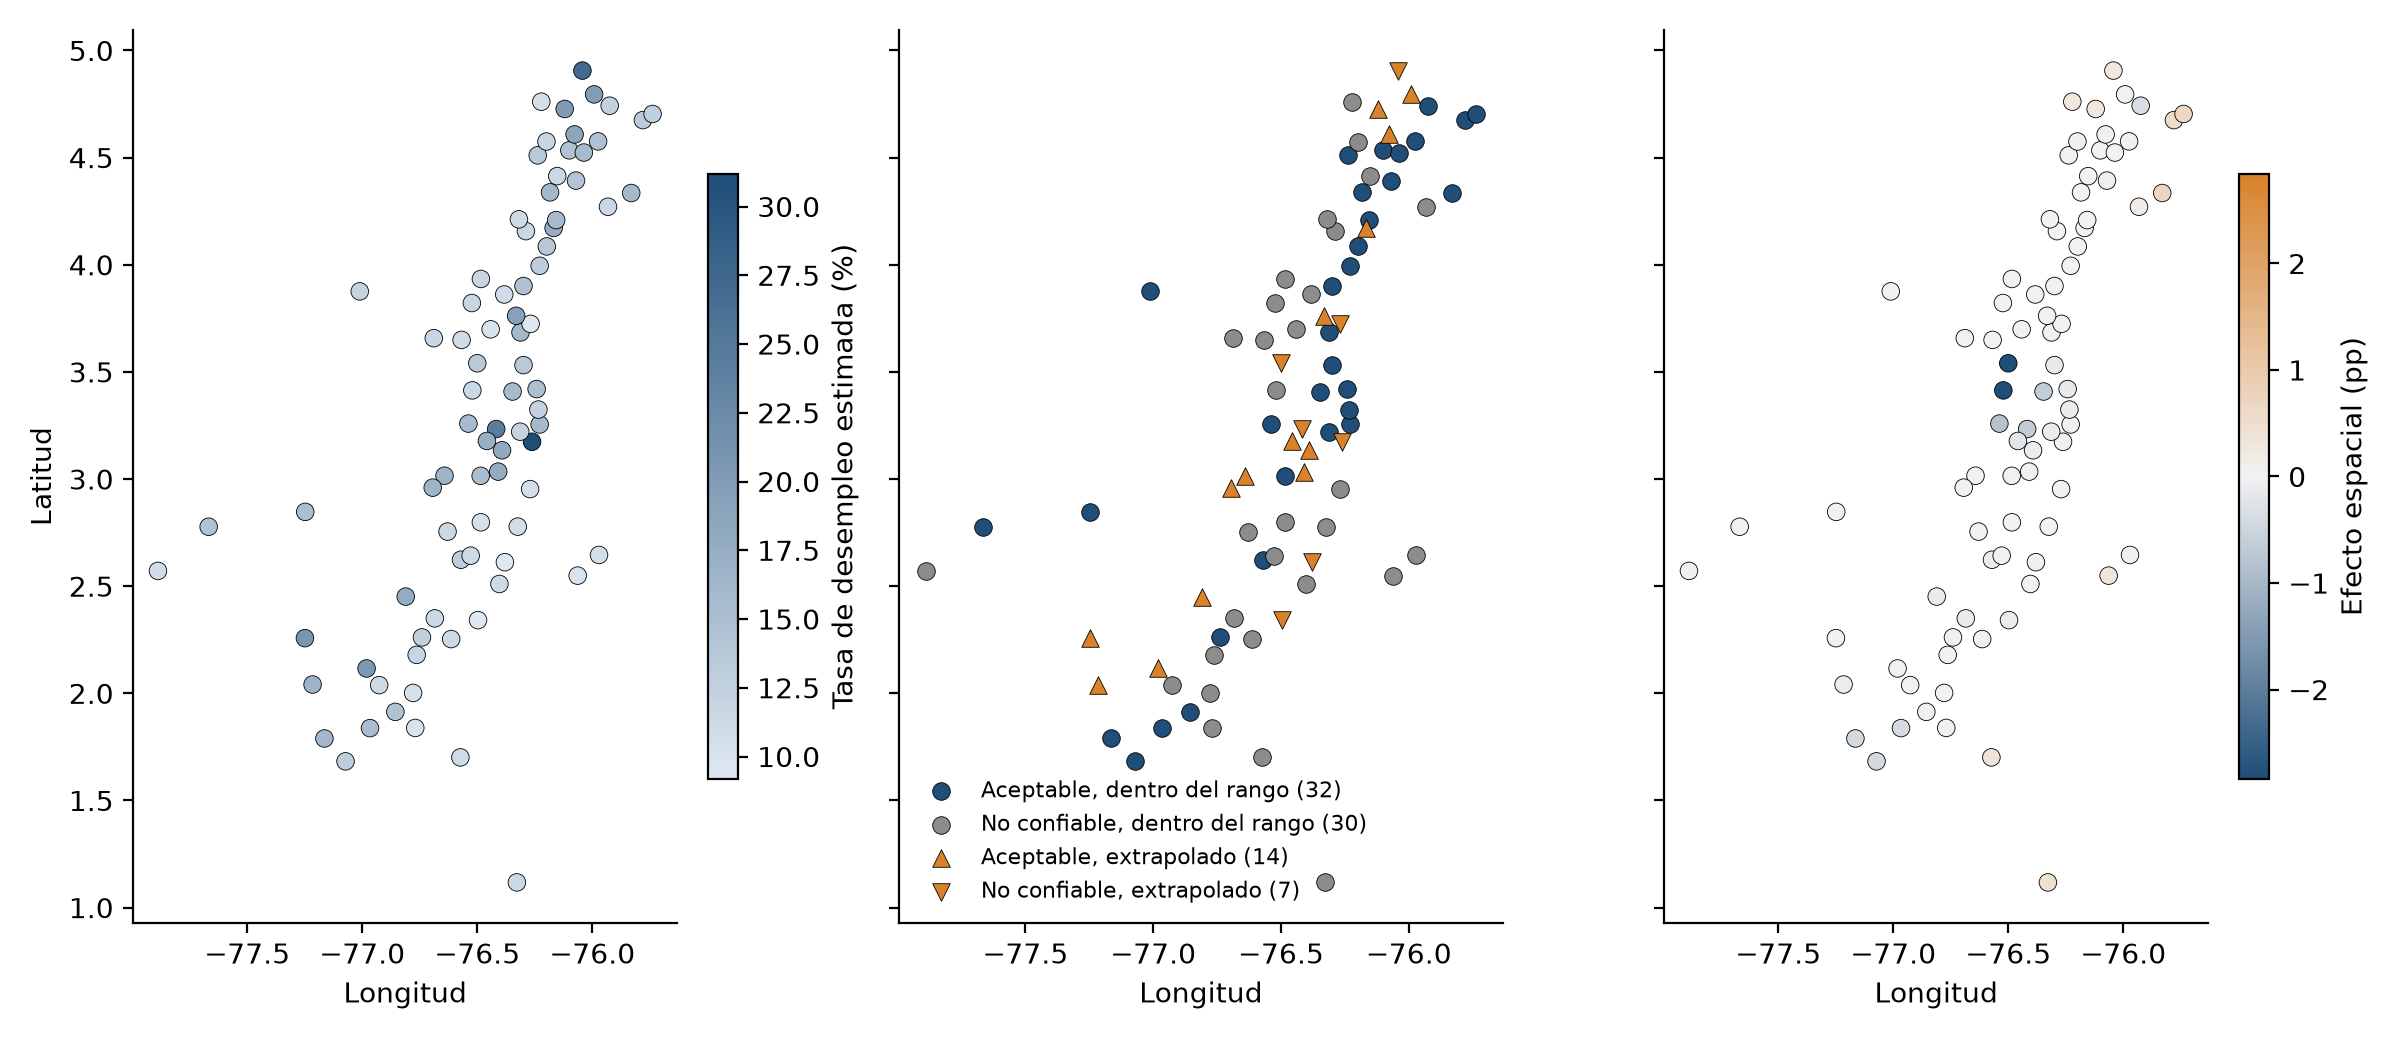
\includegraphics[width=\linewidth]{img/res_mapa_municipios.png}
\caption{Municipios objetivo ubicados en su cabecera. Izquierda: tasa de desempleo estimada en la tabla final. Centro: clase de CV y estado de extrapolación. Derecha: efecto espacial del escenario de referencia (estimación espacial menos sintética). Fuente: tabla final consolidada y tabla de estimaciones de los municipios objetivo del modelo espacial.}
\label{fig:res_mapa_municipios}
\end{figure}

Las estimaciones finales tienen autocorrelación espacial positiva: con 3 vecinos, el I de Moran es 0.265 ($E[I] = -0.012$; $p = 0.001$ con \num{9999} permutaciones). El patrón viene de la covariable: la tasa de homicidios de los mismos 83 municipios, con la misma matriz, tiene $I = 0.256$ y el mismo $p$, y la estimación sin benchmarking da prácticamente el mismo valor (0.256), porque es una función lineal de esa tasa. El efecto espacial no agrega un patrón propio: es menor que 0.5 puntos porcentuales en 75 de los 83 municipios y solo es grande en Cali y Yumbo, por el efecto de su dominio. Por eso, los grupos del mapa reflejan dónde hubo más homicidios en 2018, no un patrón del desempleo observado en esos municipios.

%--------------------------------------------------------------------------------------
\section{Correspondencia entre etapas y objetivos}
\label{sec:res_objetivos}

La Tabla~\ref{tab:res_objetivos} reúne, para cada objetivo, la evidencia principal de este capítulo, en el orden de la Tabla~\ref{tab:met_objetivos}.

\begin{table}[!htbp]
\centering
\small
\caption{Evidencia de Resultados por objetivo. OG: objetivo general; OE: objetivo específico.}
\label{tab:res_objetivos}
\begin{tabularx}{\linewidth}{>{\raggedright\arraybackslash}p{1.4cm} >{\raggedright\arraybackslash}X >{\raggedright\arraybackslash}p{3.4cm}}
\toprule
Objetivo & Resultado principal & Evidencia \\
\midrule
OG & Procedimiento completo y reproducible de 16 etapas; 23 dominios con directa confiable y validada contra el DANE; 83 municipios con estimación, ECM, estado de extrapolación y calidad reportada & Tablas~\ref{tab:res_directa}, \ref{tab:res_calidad}; Apéndice~\ref{app:municipios} \\
OE1 & Benchmark EC3; ocho especificaciones espaciales sin evidencia de $\rho \neq 0$ ($p \geq 0.221$) ni Moran significativo; estimaciones prácticamente iguales en dominios y con diferencia absoluta media de 0.22 puntos en municipios & Tablas~\ref{tab:res_espacial}, \ref{tab:res_moran}, \ref{tab:res_comparacion} \\
OE2 & Una covariable, la tasa de homicidios ($\hat{\beta} = 0.099$), asociada positivamente con la tasa; depende de Quibdó y el procedimiento completo estima peor que el modelo nulo (habilidad $-0.54$) & Tablas~\ref{tab:res_coeficientes}, \ref{tab:res_estabilidad}, \ref{tab:res_validacion} \\
OE3 & Tasas más altas en el norte del Cauca y el norte del Valle, todas extrapoladas; Moran de 0.265 que repite el de la tasa de homicidios; efecto espacial menor que 0.5 puntos en 75 de 83 & Figura~\ref{fig:res_mapa_municipios}; Sección~\ref{sec:res_patrones} \\
\bottomrule
\end{tabularx}
\end{table}
\FloatBarrier

    % --------------------------
    \chapter{Discusión y trabajo futuro}
        

\label{sec:discusion}

\section{Discusión}

\begin{itemize}
    \item Objetivo 1: 
    \item Objetivo 2:
    \item Objetivo 3:
\end{itemize}

\section{Trabajo futuro}
   % --------------------------
    \chapter{Conclusiones}
        
\label{sec:conclusion}

Las conclusiones se organizan por objetivo. Cada una se apoya en una cifra de la Sección~\ref{sec:resultados} y su alcance se discute en la Sección~\ref{sec:discusion}.

%--------------------------------------------------------------------------------------
\section{Conclusión asociada al objetivo general}

El objetivo general pedía una metodología para estimar la tasa de desempleo de los municipios del Cauca y del Valle del Cauca con estimación de áreas pequeñas, integrando varias fuentes y covariables con respaldo en la literatura. Se desarrolló y se aplicó al año 2018: un procedimiento de 16 etapas que integra la GEIH, TerriData, la DIVIPOLA y las cifras publicadas por el DANE, y que entrega una estimación para cada uno de los 83 municipios objetivo con su error, su estado de extrapolación y una calidad reportada.

El procedimiento reproduce las cifras oficiales donde existen. Las tasas directas de los 23 dominios coinciden con las del DANE, con una diferencia máxima de 0.0005 puntos porcentuales, y la tasa conjunta, 10.83~\%, es la del total de 23 ciudades y áreas metropolitanas. Los 23 dominios quedan como confiables, con CV entre 2.01~\% y 3.23~\%.

Las estimaciones municipales, en cambio, tienen un alcance limitado. Ninguno de los 83 municipios queda como confiable: 46 son aceptables y 37 no confiables por su CV, que va de 18.07~\% a 30.03~\%. De ellos, 21 son extrapolación del modelo, y todos dependen del supuesto de que la relación estimada en 23 dominios urbanos vale para municipios con una población urbana mediana de 45.07~\%. El aporte del trabajo es, por eso, la metodología y no las cifras: un procedimiento reproducible que dice con qué calidad y bajo qué supuestos se puede estimar el desempleo de un municipio sin encuesta, y que puede repetirse con mejores covariables u otros años.

%--------------------------------------------------------------------------------------
\section{Conclusión asociada al objetivo específico 1}

El primer objetivo específico pedía evaluar el desempeño de modelos de áreas pequeñas con componentes espaciales. Se compararon el Fay-Herriot clásico, elegido entre cuatro especificaciones candidatas, y ocho especificaciones espaciales SAR, con cuatro matrices de proximidad por distancia y dos estructuras. Todas usan la misma respuesta, los mismos $\psi_d$, los mismos 23 dominios y la misma covariable.

Los datos no dieron evidencia de dependencia espacial: ninguna especificación tiene un LRT de $\rho = 0$ significativo ($p \geq 0.221$), el I de Moran de los residuos no es significativo ni en el clásico (I de 0.093 con 3 vecinos, $p = 0.333$) ni en el espacial, y el AIC del espacial es mayor en todos los casos. En los dominios las dos estimaciones son prácticamente iguales (diferencia máxima de 0.02 puntos porcentuales y CV mediano de 2.60~\% en ambos); en los municipios la diferencia absoluta media es 0.22 puntos. El modelo recomendado es el Fay-Herriot clásico con la tasa de homicidios, y el espacial queda como análisis de sensibilidad. Con 23 ciudades dispersas la prueba tiene poca potencia, de modo que el resultado dice que estos datos no justifican el componente espacial, no que el desempleo municipal carezca de estructura espacial.

%--------------------------------------------------------------------------------------
\section{Conclusión asociada al objetivo específico 2}

El segundo objetivo específico pedía determinar las variables con mayor incidencia en la tasa de desempleo. De 18 candidatas con respaldo en la literatura, la única que quedó en el modelo es la tasa de homicidios, con una asociación positiva: 0.099 puntos porcentuales más de desempleo por cada homicidio adicional por 100,000 habitantes (error estándar de 0.036), que se mantiene casi igual en el modelo espacial (0.102). Es una asociación estadística condicional a la selección, no un efecto causal.

Esa asociación es frágil. Explica el 27~\% de la variación entre dominios, depende de un solo dominio (sin Quibdó baja un 38~\% y deja de ser significativa) y no se sostiene cuando la selección se repite sin cada dominio: el procedimiento completo produce seis conjuntos distintos y estima peor que el modelo de solo intercepto (RMSE de 3.43 frente a 2.77 puntos porcentuales). La conclusión es que las covariables municipales disponibles en TerriData explican poco de las diferencias de desempleo entre ciudades, y que mejorar las covariables es la condición para que el modelo aporte más que el promedio de los dominios.

%--------------------------------------------------------------------------------------
\section{Conclusión asociada al objetivo específico 3}

El tercer objetivo específico pedía analizar la distribución y los patrones espaciales del desempleo municipal a partir de las estimaciones. Las 83 estimaciones van de 9.19~\% a 31.17~\%, con mediana de 13.29~\%; el Cauca y el Valle del Cauca tienen promedios casi iguales (14.16~\% y 14.18~\%), pero el Cauca es más disperso y tiene más municipios que extrapolan (13 de 41 frente a 8 de 42). Las tasas más altas se concentran en el norte del Cauca y en el norte del Valle, todas en municipios que extrapolan.

Las estimaciones tienen autocorrelación espacial positiva (I de Moran de 0.265, $p = 0.001$), pero ese patrón es el de la tasa de homicidios, que con la misma matriz da 0.256, y el efecto espacial del modelo es menor que 0.5 puntos porcentuales en 75 de los 83 municipios. El mapa de las estimaciones describe, por tanto, la distribución territorial de la covariable usada y no una medición del desempleo en esos municipios; su lectura como patrón del desempleo queda sujeta a que la relación del modelo valga fuera de los dominios.

   % --------------------------
    \clearpage
    \printbibliography
    % --------------------------
     \begin{appendices}
     \chapter{Apéndice}
        
\label{sec:apendice}

El apéndice reúne el material de apoyo que el cuerpo del documento cita: la reproducción del procesamiento, el linaje de las tablas, los nombres de las variables, el catálogo de covariables y las tablas y figuras complementarias de cada etapa de los Resultados.

%--------------------------------------------------------------------------------------
\anexo{Disponibilidad de datos y código, y reproducción}
\label{app:reproducibilidad}

Esta sección indica dónde están los datos y el código y cómo se repite el procesamiento; la cita la Sección~\ref{sec:metodologia}.

Las cuatro fuentes son públicas: los microdatos de la GEIH y el anexo de mercado laboral se descargan del archivo nacional de datos del DANE, TerriData del portal del DNP y la DIVIPOLA del geoportal del DANE (Tabla~\ref{tab:fuentes_datos}). El código está en el repositorio \url{https://github.com/juanp001/Estimacion-desempleo-Colombia-SAE}. Todo corre en Databricks con tablas de Unity Catalog en el catálogo \texttt{tesis} y se despliega como un conjunto de trabajos programados. Con el entorno configurado, el procesamiento completo se repite con el trabajo \texttt{pipeline\_completo}, que recibe el año y el mes de cierre y el número de meses de la ventana.

La Tabla~\ref{tab:app_jobs} relaciona cada trabajo con sus tareas y con las etapas de la metodología que cubre. El trabajo del modelo escribe también las tablas de la comparación entre el Fay-Herriot espacial y el clásico que usa la Sección~\ref{sec:res_espacial}: el SEBLUP de los 23 dominios con su ECM, su CV y su peso, las diferencias entre las dos estimaciones en dominios y municipios, y el índice de Moran de las 83 estimaciones municipales. Las dos figuras de esa comparación y el mapa municipal no salen de los trabajos: las dibuja el guion \texttt{img/\_script/figuras\_resultados.py}, versionado junto con el documento, que lee esas tablas sin recalcular ninguna cifra.

Las cifras del documento corresponden a la corrida del 31 de octubre de 2026 de la ingesta y el preprocesamiento y a la del 5 de noviembre de 2026 del análisis y el modelo, con la versión del repositorio etiquetada \texttt{documento-v1}.

\begin{table}[!htbp]
\centering
\small
\caption[Trabajos programados del procesamiento]{Trabajos programados del procesamiento y etapas de la metodología que cubren. La sensibilidad a la ventana temporal (etapa 5) se ejecuta aparte. GEIH: Gran Encuesta Integrada de Hogares; DANE: Departamento Administrativo Nacional de Estadística; DIVIPOLA: División Político-Administrativa de Colombia.}
\label{tab:app_jobs}
\begin{adjustbox}{max width=\linewidth}
\begin{tabular}{l p{8.6cm} l}
\toprule
Trabajo & Tareas & Etapas \\
\midrule
dimensiones & Tabla de la DIVIPOLA; dominios de la GEIH y sus municipios; capitales con coordenadas & 4 \\
ingesta\_geih & Capas bronce, plata y oro de la GEIH; cifras publicadas por el DANE & 1, 2 \\
ingesta\_terridata & Capas bronce y plata de TerriData; diccionario de indicadores & 1, 2 \\
preprocesamiento & Estimación directa; covariables por dominio y auditoría; pre-filtrado; municipios objetivo & 5 a 7 \\
analisis & Análisis descriptivo; selección de covariables y su sensibilidad al umbral $q$ & 8, 9 \\
modelo & Fay-Herriot clásico; Fay-Herriot espacial y tablas de su comparación con el clásico; sensibilidad a la varianza & 10 a 16 \\
pipeline\_completo & Ejecuta los seis trabajos anteriores en orden & 1 a 16 \\
\midrule
\multicolumn{3}{l}{Fuera de los trabajos} \\
\texttt{figuras\_resultados.py} & Figuras de la comparación espacial y mapa de los 83 municipios, a partir de las tablas del trabajo del modelo & 13, 16 \\
\bottomrule
\end{tabular}
\end{adjustbox}
\end{table}
%--------------------------------------------------------------------------------------
\anexo{Linaje de tablas}
\label{app:linaje}

Esta sección relaciona cada tabla del procesamiento con el cuaderno que la escribe y la etapa de la metodología; la citan las Secciones~\ref{sec:metodologia} y~\ref{sec:resultados}.

La Tabla~\ref{tab:app_linaje} se lee de arriba abajo en el orden en que corre el procesamiento: las capas de la GEIH y de TerriData alimentan la estimación directa y las covariables, y estas al modelo, que escribe la tabla final. Con ella se puede ubicar el cuaderno que produce cada cifra de los Resultados.

{\footnotesize\setlength{\tabcolsep}{3pt}
\begin{longtable}{p{2.8cm} p{3.6cm} p{4.8cm} p{1.2cm}}
\caption[Linaje de las tablas del procesamiento]{Linaje de las tablas del catálogo de Unity Catalog del trabajo, de la ingesta a la tabla final. GEIH: Gran Encuesta Integrada de Hogares; DIVIPOLA: División Político-Administrativa de Colombia; EBLUP: mejor predictor lineal insesgado empírico; GVF: función generalizada de varianza.}
\label{tab:app_linaje} \\
\toprule
Esquema & Contenido & Cuaderno & Etapa \\
\midrule
\endfirsthead
\multicolumn{4}{l}{\tablename~\thetable{}, continuación} \\
\toprule
Esquema & Contenido & Cuaderno & Etapa \\
\midrule
\endhead
\bottomrule
\endlastfoot
\texttt{geih\_bronce} & Un archivo por módulo y sección (cabecera y resto del marco antiguo; un archivo por módulo en el marco nuevo) y el factor de expansión recalculado & \texttt{geih\_bronce} & 1 \\
\texttt{geih\_bronce} & Cifras publicadas: nacionales, por ciudad (trimestre móvil) y anuales & \texttt{datos\_publicados} & 1 \\
\texttt{geih\_plata} & Un módulo consolidado por tabla (características generales, fuerza de trabajo, ocupados, no ocupados) y factores de expansión & \texttt{geih\_plata} & 2 \\
\texttt{geih\_oro} & Mercado laboral (una fila por persona); llaves sin pareja; reconciliación de la fuerza de trabajo & \texttt{geih\_oro} & 2 \\
\texttt{terridata} & Indicadores en formato largo (bronce) y ancho (plata) & \texttt{terridata\_bronce, terridata\_plata} & 1, 2 \\
\texttt{dim} & DIVIPOLA; dominios de la GEIH; capitales con coordenadas; diccionario de indicadores & \texttt{dim\_divipola, dim\_dominio\_geih, dim\_geih\_divipola, terridata\_plata} & 1, 4 \\
\texttt{preprocesamiento} & Tasa directa por dominio; sensibilidad de la ventana & \texttt{estimacion\_directa, sensibilidad\_ventana\_temporal} & 5 \\
\texttt{preprocesamiento} & Tasa con covariables; reglas de agregación; auditoría de dominios & \texttt{adicion\_covariables} & 4, 6 \\
\texttt{preprocesamiento} & Covariables pre-filtradas; cascada; sensibilidad de la variabilidad; municipios objetivo & \texttt{pre\_filtrado\_covariables, dominios\_sin\_encuesta} & 6, 7 \\
\texttt{preprocesamiento} & Catálogo; descriptivo univariado y bivariado & \texttt{analisis\_descriptivo} & 8 \\
\texttt{preprocesamiento} & Diagnósticos, soporte, redundancia, decisión, verificación, trazabilidad, conjunto seleccionado y sensibilidad al umbral $q$ & \texttt{eda\_seleccion\_covariables} & 9 \\
\texttt{modelo} & Especificaciones, coeficientes, Cook, estabilidad, validación, extrapolación, EBLUP, estimación sintética y tabla final & \texttt{fay\_herriot} & 10 a 12, 14, 15 \\
\texttt{modelo} & Comparación espacial, Moran de los residuos y de las estimaciones municipales, perfil de $\rho$, validación, coeficientes, SEBLUP de los dominios, diferencias frente al clásico, sensibilidades y estimación de los municipios & \texttt{fay\_herriot\_espacial} & 13, 14, 16 \\
\texttt{modelo} & Varianzas alternativas, GVF y escenarios & \texttt{sensibilidad\_varianza} & 11 \\
\end{longtable}
}
El catálogo tiene 92 tablas escritas por el código vigente, repartidas así: dim, 4; geih\_bronce, 18; geih\_oro, 3; geih\_plata, 5; modelo, 38; preprocesamiento, 22; terridata, 2. Quedan además en el catálogo tablas de versiones anteriores que ningún cuaderno vigente lee ni escribe: las del censo, las de la sección de área del marco antiguo, una lista de candidatas y una tabla de robustez de covariables, y una dimensión de tiempo.

%--------------------------------------------------------------------------------------
\anexo{Nombres de las variables y de los modelos}
\label{app:variables}

Esta sección relaciona el nombre que usa el texto con el código de TerriData o la columna del procesamiento; la citan las Secciones~\ref{sec:datos} y~\ref{sec:resultados}.

La Tabla~\ref{tab:app_variables} es la referencia única de nombres del documento: cada covariable, columna y modelo se escribe en el texto, las tablas y las figuras con el nombre de su primera columna. El primer bloque traduce los 18 códigos de TerriData; el segundo, las columnas del procesamiento; el tercero, los nombres de los modelos y de las estimaciones.

{\footnotesize\setlength{\tabcolsep}{3pt}
\begin{longtable}{p{3.5cm} p{3.5cm} p{5.7cm}}
\caption[Nombres de las variables y de los modelos]{Nombres de las variables y de los modelos. Arriba, las 18 covariables candidatas con su código de TerriData; en medio, las columnas del procesamiento que el texto nombra en lenguaje natural; abajo, los modelos y las estimaciones. CV: coeficiente de variación; ECM: error cuadrático medio; EBLUP: mejor predictor lineal insesgado empírico; PEA: población económicamente activa; GEIH: Gran Encuesta Integrada de Hogares; CNPV: Censo Nacional de Población y Vivienda; DIVIPOLA: División Político-Administrativa de Colombia.}
\label{tab:app_variables} \\
\toprule
Nombre en el documento & Código o columna & Descripción \\
\midrule
\endfirsthead
\multicolumn{3}{l}{\tablename~\thetable{}, continuación} \\
\toprule
Nombre en el documento & Código o columna & Descripción \\
\midrule
\endhead
\bottomrule
\endlastfoot
Penetración de banda ancha & 030010003 & Penetración de banda ancha; Porcentaje (el valor está multiplicado por 100) \\
Cobertura de acueducto & 030010004 & Cobertura de acueducto (Censo); Porcentaje (el valor está multiplicado por 100) \\
Cobertura neta en educación media & 040010010 & Cobertura neta en educación media; Porcentaje (el valor está multiplicado por 100) \\
Cobertura neta en educación secundaria & 040010009 & Cobertura neta en educación secundaria; Porcentaje (el valor está multiplicado por 100) \\
Densidad de población & 010010010 & Densidad poblacional; Hab/Km2 \\
Índice de desempeño fiscal & 070100007 & Indicador de desempeño fiscal; Puntos \\
Índice de pobreza multidimensional & 140010004 & Índice de pobreza multidimensional - IPM; Porcentaje (el valor está multiplicado por 100) \\
Ingresos tributarios per cápita & 070010020 & Ingresos tributarios per cápita; Pesos corrientes \\
Población joven de 14 a 28 años & 020090021 & Porcentaje de población de jóvenes entre 14 y 28 años; Porcentaje \\
Población urbana & 020040003 & Porcentaje población urbana; Porcentaje (el valor está multiplicado por 100) \\
Saber 11, lectura crítica & 040040002 & Puntaje promedio Pruebas Saber 11 - Lectura crítica; Puntos \\
Saber 11, matemáticas & 040040001 & Puntaje promedio Pruebas Saber 11 - Matemáticas; Puntos \\
Tasa de homicidios & 060010003 & Tasa de homicidios por cada 100,000 habitantes \\
Tránsito a la educación superior & 040010028 & Tasa de tránsito inmediato a la educación superior; Porcentaje \\
Valor agregado per cápita & 120210002 & Valor agregado per cápita; Pesos corrientes \\
Valor agregado de actividades primarias & 120210008 & Porcentaje del valor agregado por actividades económicas - Actividades primarias; Porcentaje \\
Valor agregado de actividades secundarias & 120210009 & Porcentaje del valor agregado por actividades económicas - Actividades secundarias; Porcentaje \\
Valor agregado de actividades terciarias & 120210010 & Porcentaje del valor agregado por actividades económicas - Actividades terciarias; Porcentaje \\
\midrule
Tasa de desempleo directa & \texttt{TASA\_DESEMPLEO\_PCT} & Estimador de Hájek de la tasa de desempleo del dominio, en \% \\
Error estándar bootstrap & \texttt{SE\_BOOTSTRAP\_PCT} & Desviación de 2,000 réplicas por viviendas, en puntos porcentuales; $\psi_d$ es su cuadrado \\
Error estándar de Taylor & \texttt{SE\_TAYLOR\_PCT} & Linealización de la razón con las mismas viviendas \\
Factor de expansión & \texttt{FEX\_C18} & Peso de la persona calibrado con el CNPV 2018 \\
Vivienda & \texttt{ID\_VIVIENDA} & Período más directorio; conglomerado del bootstrap \\
Código de área & \texttt{AREA} & Departamento de la ciudad del dominio en la GEIH \\
Dominio & \texttt{CODIGO\_DOMINIO} & DIVIPOLA de la capital del dominio \\
PEA expandida & \texttt{PEA\_EXPANDIDA} & Suma de factores de la PEA dividida por los meses; peso del benchmarking de nivel 1 \\
Peso de la directa & \texttt{GAMMA\_SHRINKAGE} & $\hat{\gamma}_d$ del EBLUP \\
EBLUP y su ECM & \texttt{EBLUP, MSE\_EBLUP} & Estimación del Fay-Herriot clásico y su ECM de Prasad-Rao \\
Estado de extrapolación & \texttt{ESTADO\_EXTRAPOLACION} & Dentro del rango, fuera del rango o combinación atípica \\
Calidad reportada & \texttt{CALIDAD\_REPORTADA} & Clase de CV más «condicional al modelo» y «extrapolado» si corresponde \\
\midrule
Fay-Herriot clásico & \texttt{FayHerriotClasico} & Modelo de área sin componente espacial; sus especificaciones candidatas son EC0 a EC3 \\
Benchmark (EC3) & \texttt{modelo\_ganador} & Especificación elegida del Fay-Herriot clásico, con la tasa de homicidios; se nombra «benchmark» o «EC3» \\
Modelo de solo intercepto (EC0) & EC0 & Especificación sin covariables; «habilidad frente al nulo» es la única expresión que conserva la palabra «nulo» \\
Fay-Herriot espacial & \texttt{FayHerriotEspacial} & Modelo con efectos de área autorregresivos simultáneos; su estimación en los dominios es el SEBLUP \\
Estimación sintética & \texttt{PRED\_SINTETICO} & $\mathbf{x}^\top\hat{\boldsymbol{\beta}}$ en un municipio sin muestra; la fórmula que la produce es el predictor sintético \\
Estimación espacial & \texttt{PRED\_ESPACIAL} & Resultado del Fay-Herriot espacial en un municipio, escenario de referencia; la fórmula es el predictor espacial \\
\end{longtable}
}
%--------------------------------------------------------------------------------------
\anexo{Catálogo de covariables}
\label{app:catalogo}

Esta sección lista las entradas del catálogo de literatura con su código, el signo esperado y la referencia que las respalda; la citan las Secciones~\ref{sec:datos}, \ref{sec:met_covariables} y~\ref{sec:res_covariables}.

En la Tabla~\ref{tab:app_catalogo} las 18 candidatas se reparten en siete dimensiones de TerriData; la educación aporta cinco y la economía cuatro. En las tres participaciones sectoriales del valor agregado y en la densidad de población la literatura no fija un signo. Dos referencias del catálogo de origen no se pudieron localizar como documentos publicados (el número 211 de los Reportes del Emisor y el tomo social del atlas estadístico del DANE) y se dejan como texto, sin entrada en la bibliografía. El bloque final reúne las seis variables que no entraron y el motivo de cada una.

{\footnotesize\setlength{\tabcolsep}{3pt}
\begin{longtable}{p{2.8cm} p{1.5cm} p{2.0cm} p{0.8cm} p{4.6cm}}
\caption[Catálogo de covariables de la literatura]{Catálogo de literatura: 18 entradas activas y 6 sin dato utilizable o retiradas. Signo: relación esperada con la tasa de desempleo ($\pm$: sin signo definido). TD: tasa de desempleo; DANE: Departamento Administrativo Nacional de Estadística; IICA: índice de incidencia del conflicto armado.}
\label{tab:app_catalogo} \\
\toprule
Covariable & Código & Dimensión & Signo & Referencia o motivo \\
\midrule
\endfirsthead
\multicolumn{5}{l}{\tablename~\thetable{}, continuación} \\
\toprule
Covariable & Código & Dimensión & Signo & Referencia o motivo \\
\midrule
\endhead
\bottomrule
\endlastfoot
Cobertura neta en educación media & 040010010 & Educación & $-$ & Castillo-Robayo y García-Estévez \cite{CastilloGarcia2019} \\
Cobertura neta en educación secundaria & 040010009 & Educación & $-$ & Castillo-Robayo y García-Estévez \cite{CastilloGarcia2019} \\
Saber 11, matemáticas & 040040001 & Educación & $-$ & Castillo-Robayo y García-Estévez \cite{CastilloGarcia2019} \\
Saber 11, lectura crítica & 040040002 & Educación & $-$ & Castillo-Robayo y García-Estévez \cite{CastilloGarcia2019} \\
Tránsito a la educación superior & 040010028 & Educación & $-$ & Castillo-Robayo y García-Estévez \cite{CastilloGarcia2019}, por el mecanismo de capital humano; se conservó por decisión del equipo \\
Valor agregado per cápita & 120210002 & Economía & $-$ & Rubio Ugalde, Lara Gómez y Hurtado Maldonado \cite{RubioUgalde2025} \\
Valor agregado de actividades primarias & 120210008 & Economía & $\pm$ & Bonet \cite{Bonet2005}; Reportes del Emisor n.º 211, Banco de la República (2016), sin localizar \\
Valor agregado de actividades secundarias & 120210009 & Economía & $\pm$ & Bonet \cite{Bonet2005}; Reportes del Emisor n.º 211, Banco de la República (2016), sin localizar \\
Valor agregado de actividades terciarias & 120210010 & Economía & $\pm$ & Bonet \cite{Bonet2005}; Reportes del Emisor n.º 211, Banco de la República (2016), sin localizar \\
Índice de pobreza multidimensional & 140010004 & Pobreza & $+$ & DANE \cite{DANE_IPM2020} \\
Población urbana & 020040003 & Demografía y población & $+$ & DANE, Atlas estadístico, tomo II (social), sección «7.4. Tasa de desempleo (TD)», sin localizar \\
Densidad de población & 010010010 & Demografía y población & $\pm$ & DNP \cite{DNP_EIG01_2020}, variables de capacidades iniciales \\
Población joven de 14 a 28 años & 020090021 & Demografía y población & $+$ & Tamayo \cite{Tamayo2008} \\
Índice de desempeño fiscal & 070100007 & Finanzas públicas & $-$ & DNP \cite{DNP_IDF2024} \\
Ingresos tributarios per cápita & 070010020 & Finanzas públicas & $-$ & Fundación Felipe González \cite{FFG2021} \\
Tasa de homicidios & 060010003 & Conflicto armado y seguridad ciudadana & $+$ & Pinzón-Flórez, Díaz Rivadeneira y Escobar Morales \cite{PinzonFlorez2025} \\
Cobertura de acueducto & 030010004 & Vivienda y acceso a servicios públicos & $-$ & DNP \cite{DNP_Cartilla2019}, dimensión de vivienda y acceso a servicios públicos \\
Penetración de banda ancha & 030010003 & Vivienda y acceso a servicios públicos & $-$ & DNP \cite{DNP_Cartilla2019}, dimensión de vivienda y acceso a servicios públicos \\
\midrule
\multicolumn{5}{l}{Entradas sin dato utilizable o retiradas} \\
Tasa de analfabetismo (censo) & 040030003 & Educación & no aplica & Sin dato en los dominios con encuesta para 2018 \\
Empresas generadoras de empleo formal por cada 10,000 habitantes & 160080001 & Economía & no aplica & La serie termina en 2016 \\
Incidencia de la pobreza monetaria & 140060001 & Pobreza & no aplica & Solo departamentos y 23 ciudades; no existe en los municipios objetivo \\
Coeficiente de Gini & 140010003 & Pobreza & no aplica & Solo departamental \\
Víctimas de desplazamiento forzado ubicadas & 260030002 & Conflicto armado y seguridad ciudadana & no aplica & Solo 2022 y 2023 \\
IICA & 260020003 & Conflicto armado y seguridad ciudadana & no aplica & Retirado: mide el conflicto en el propio municipio y no la llegada de población desplazada; $r = 0.92$ con la tasa de homicidios en los dominios; 13 valores distintos \\
\end{longtable}
}
%--------------------------------------------------------------------------------------
\anexo{Auditoría de los dominios}
\label{app:auditoria}

Esta sección detalla, por dominio, la correspondencia entre la geografía de la GEIH y la de las covariables; la cita la Sección~\ref{sec:res_dominios}.

La Tabla~\ref{tab:app_auditoria} muestra que en los 23 dominios la tasa directa coincide con la cifra publicada por el DANE con dos decimales. Los siete dominios con área metropolitana toman sus covariables como razón de totales de sus municipios miembro; los otros 16 usan el valor del municipio.

{\footnotesize\setlength{\tabcolsep}{3pt}
\begin{longtable}{p{2.0cm} p{1.0cm} p{1.7cm} p{2.3cm} p{1.9cm} r r}
\caption[Auditoría de los dominios de estimación]{Auditoría de los 23 dominios, Ene-Dic 2018. Área: código de área de la GEIH; DIVIPOLA: código de la capital; Covariables: valor municipal o razón de totales con el denominador propio (Ecuación~\ref{eq:agregacion}); TD: tasa de desempleo, en \%; DANE: Departamento Administrativo Nacional de Estadística; A.M.: área metropolitana. La tasa describe las cabeceras y las covariables el municipio completo.}
\label{tab:app_auditoria} \\
\toprule
Dominio & Área & DIVIPOLA & Municipios & Covariables & TD & TD DANE \\
\midrule
\endfirsthead
\multicolumn{7}{l}{\tablename~\thetable{}, continuación} \\
\toprule
Dominio & Área & DIVIPOLA & Municipios & Covariables & TD & TD DANE \\
\midrule
\endhead
\bottomrule
\endlastfoot
Armenia & 63 & 63001 & Armenia & Valor municipal & 15.49 & 15.49 \\
Barranquilla A.M. & 08 & 08001 & Barranquilla, Soledad & Razón de totales & 8.15 & 8.15 \\
Bogotá & 11 & 11001 & Bogotá, D.C. & Valor municipal & 10.37 & 10.37 \\
Bucaramanga A.M. & 68 & 68001 & Bucaramanga, Floridablanca, Girón, Piedecuesta & Razón de totales & 8.74 & 8.74 \\
Cali A.M. & 76 & 76001 & Santiago de Cali, Yumbo & Razón de totales & 11.65 & 11.65 \\
Cartagena & 13 & 13001 & Cartagena de Indias & Valor municipal & 8.35 & 8.35 \\
Cúcuta A.M. & 54 & 54001 & San José de Cúcuta, El Zulia, Los Patios, Villa del Rosario & Razón de totales & 15.98 & 15.98 \\
Florencia & 18 & 18001 & Florencia & Valor municipal & 12.94 & 12.94 \\
Ibagué & 73 & 73001 & Ibagué & Valor municipal & 13.99 & 13.99 \\
Manizales A.M. & 17 & 17001 & Manizales, Villamaría & Razón de totales & 11.24 & 11.24 \\
Medellín A.M. & 05 & 05001 & Medellín, Barbosa, Bello, Caldas, Copacabana, Envigado, Girardota, Itagüí, La Estrella, Sabaneta & Razón de totales & 11.84 & 11.84 \\
Montería & 23 & 23001 & Montería & Valor municipal & 9.47 & 9.47 \\
Neiva & 41 & 41001 & Neiva & Valor municipal & 11.53 & 11.53 \\
Pasto & 52 & 52001 & Pasto & Valor municipal & 8.82 & 8.82 \\
Pereira A.M. & 66 & 66001 & Pereira, Dosquebradas, La Virginia & Razón de totales & 8.87 & 8.87 \\
Popayán & 19 & 19001 & Popayán & Valor municipal & 10.68 & 10.68 \\
Quibdó & 27 & 27001 & Quibdó & Valor municipal & 17.81 & 17.81 \\
Riohacha & 44 & 44001 & Riohacha & Valor municipal & 13.88 & 13.88 \\
Santa Marta & 47 & 47001 & Santa Marta & Valor municipal & 8.32 & 8.32 \\
Sincelejo & 70 & 70001 & Sincelejo & Valor municipal & 9.61 & 9.61 \\
Tunja & 15 & 15001 & Tunja & Valor municipal & 11.31 & 11.31 \\
Valledupar & 20 & 20001 & Valledupar & Valor municipal & 14.45 & 14.45 \\
Villavicencio & 50 & 50001 & Villavicencio & Valor municipal & 11.87 & 11.87 \\
\end{longtable}
}
%--------------------------------------------------------------------------------------
\anexo{Análisis descriptivo de las candidatas}
\label{app:descriptivo}

Esta sección reúne la estadística univariada de las 18 candidatas y las figuras del análisis descriptivo; la cita la Sección~\ref{sec:res_descriptivo}.

En la Tabla~\ref{tab:app_univariado} la densidad de población es la candidata más dispersa (CV de 138.50~\%) y, con la tasa de homicidios, la de mayor asimetría positiva; la cobertura de acueducto es la más asimétrica hacia la izquierda ($-3.50$), por unos pocos dominios con coberturas muy por debajo de las demás. La Figura~\ref{fig:app_territorial} ordena la tasa directa de los 23 dominios, de Quibdó (17.81~\%) a Barranquilla A.M. (8.15~\%), y la Figura~\ref{fig:app_boxplots} pone las candidatas en una misma escala para comparar su dispersión y sus valores extremos. Las Figuras~\ref{fig:app_dispersion} y~\ref{fig:app_dispersion_2} muestran la relación de la tasa con cada candidata, y la Figura~\ref{fig:app_correlacion} agrupa las candidatas que se mueven juntas: los dos puntajes de Saber 11 ($r = 0.97$), el valor agregado per cápita con los ingresos tributarios per cápita ($r = 0.93$) y las participaciones secundaria y terciaria del valor agregado, que se mueven en sentido contrario ($r = -0.91$).

{\scriptsize\setlength{\tabcolsep}{2pt}
\begin{longtable}{p{2.8cm} r r r r r r r r}
\caption[Estadística univariada de las candidatas]{Estadística univariada de las candidatas en los 23 dominios. DE: desviación estándar; CV: coeficiente de variación, en \%; Asim.: asimetría; Ext.: valores señalados por la regla del diagrama de caja (Ecuación~\ref{eq:iqr}). El valor agregado per cápita y los ingresos tributarios per cápita están en millones de pesos corrientes; la densidad, en habitantes por km$^2$.}
\label{tab:app_univariado} \\
\toprule
Covariable & Media & Mediana & DE & Mín. & Máx. & CV & Asim. & Ext. \\
\midrule
\endfirsthead
\multicolumn{9}{l}{\tablename~\thetable{}, continuación} \\
\toprule
Covariable & Media & Mediana & DE & Mín. & Máx. & CV & Asim. & Ext. \\
\midrule
\endhead
\bottomrule
\endlastfoot
Cobertura neta en educación media & 48.32 & 48.10 & 5.63 & 33.80 & 57.01 & 11.65 & $-0.76$ & 1 \\
Cobertura neta en educación secundaria & 83.79 & 84.43 & 6.18 & 75.17 & 98.36 & 7.38 & 0.59 & 0 \\
Saber 11, matemáticas & 51.56 & 52.04 & 3.21 & 43.64 & 57.49 & 6.23 & $-0.65$ & 2 \\
Saber 11, lectura crítica & 53.87 & 54.43 & 2.33 & 47.89 & 57.67 & 4.33 & $-1.00$ & 2 \\
Tránsito a la educación superior & 46.16 & 46.22 & 7.30 & 30.48 & 61.48 & 15.82 & $-0.08$ & 3 \\
Valor agregado per cápita & 15.78 & 14.91 & 5.10 & 10.00 & 30.63 & 32.32 & 1.22 & 1 \\
Valor agregado de actividades primarias & 3.35 & 2.98 & 2.77 & 0.02 & 9.54 & 82.59 & 0.81 & 0 \\
Valor agregado de actividades secundarias & 18.07 & 15.45 & 6.57 & 6.62 & 36.95 & 36.36 & 0.99 & 1 \\
Valor agregado de actividades terciarias & 78.59 & 78.74 & 6.09 & 62.95 & 86.41 & 7.75 & $-0.63$ & 0 \\
Índice de pobreza multidimensional & 20.88 & 17.60 & 9.85 & 9.00 & 45.10 & 47.17 & 1.28 & 2 \\
Población urbana & 90.19 & 92.40 & 7.58 & 67.07 & 99.87 & 8.40 & $-1.46$ & 1 \\
Densidad de población & 1,339.79 & 521.43 & 1,855.67 & 42.03 & 7,769.60 & 138.50 & 2.32 & 2 \\
Población joven de 14 a 28 años & 25.79 & 25.75 & 1.47 & 23.13 & 28.88 & 5.70 & 0.38 & 1 \\
Índice de desempeño fiscal & 76.83 & 77.23 & 3.63 & 68.79 & 85.32 & 4.73 & 0.02 & 0 \\
Ingresos tributarios per cápita & 0.42 & 0.35 & 0.21 & 0.11 & 1.10 & 50.61 & 1.47 & 1 \\
Tasa de homicidios & 23.55 & 21.38 & 14.12 & 4.06 & 71.96 & 59.98 & 2.26 & 2 \\
Cobertura de acueducto & 90.33 & 95.94 & 15.89 & 25.21 & 99.48 & 17.60 & $-3.50$ & 3 \\
Penetración de banda ancha & 17.28 & 17.69 & 4.71 & 7.59 & 24.11 & 27.27 & $-0.23$ & 0 \\
\end{longtable}
}
\begin{figure}[!htbp]
\centering
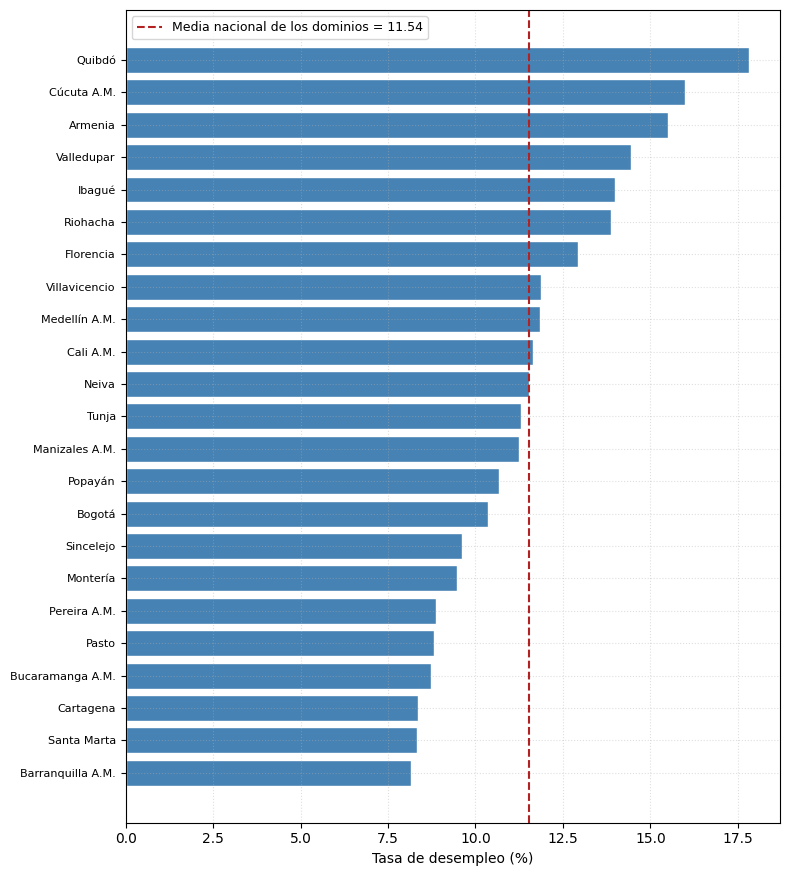
\includegraphics[width=0.9\linewidth]{img/desc_territorial_respuesta.png}
\caption{Tasa directa de los 23 dominios ordenada de mayor a menor, con su intervalo del 95~\%. Fuente: tablas del análisis descriptivo.}
\label{fig:app_territorial}
\end{figure}
\begin{figure}[!htbp]
\centering
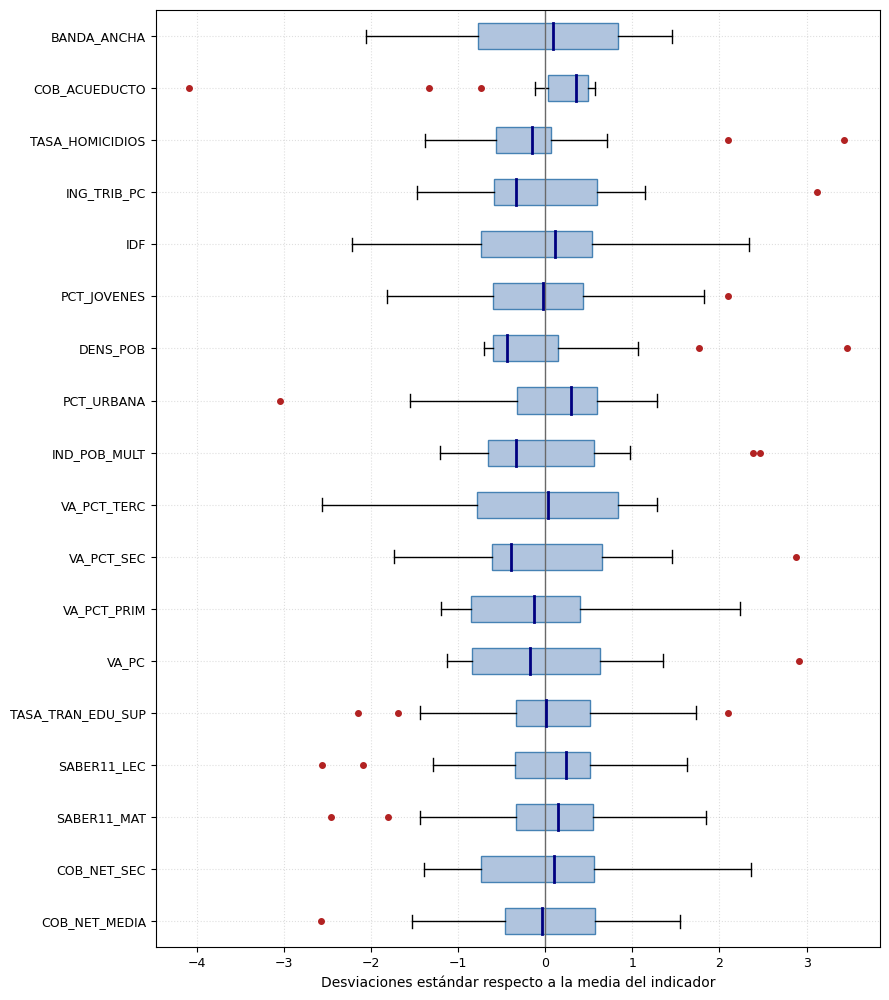
\includegraphics[width=0.9\linewidth]{img/desc_boxplots_candidatas.png}
\caption{Diagramas de caja de las 18 candidatas en escala estandarizada. Fuente: tablas del análisis descriptivo.}
\label{fig:app_boxplots}
\end{figure}
\begin{figure}[!htbp]
\centering
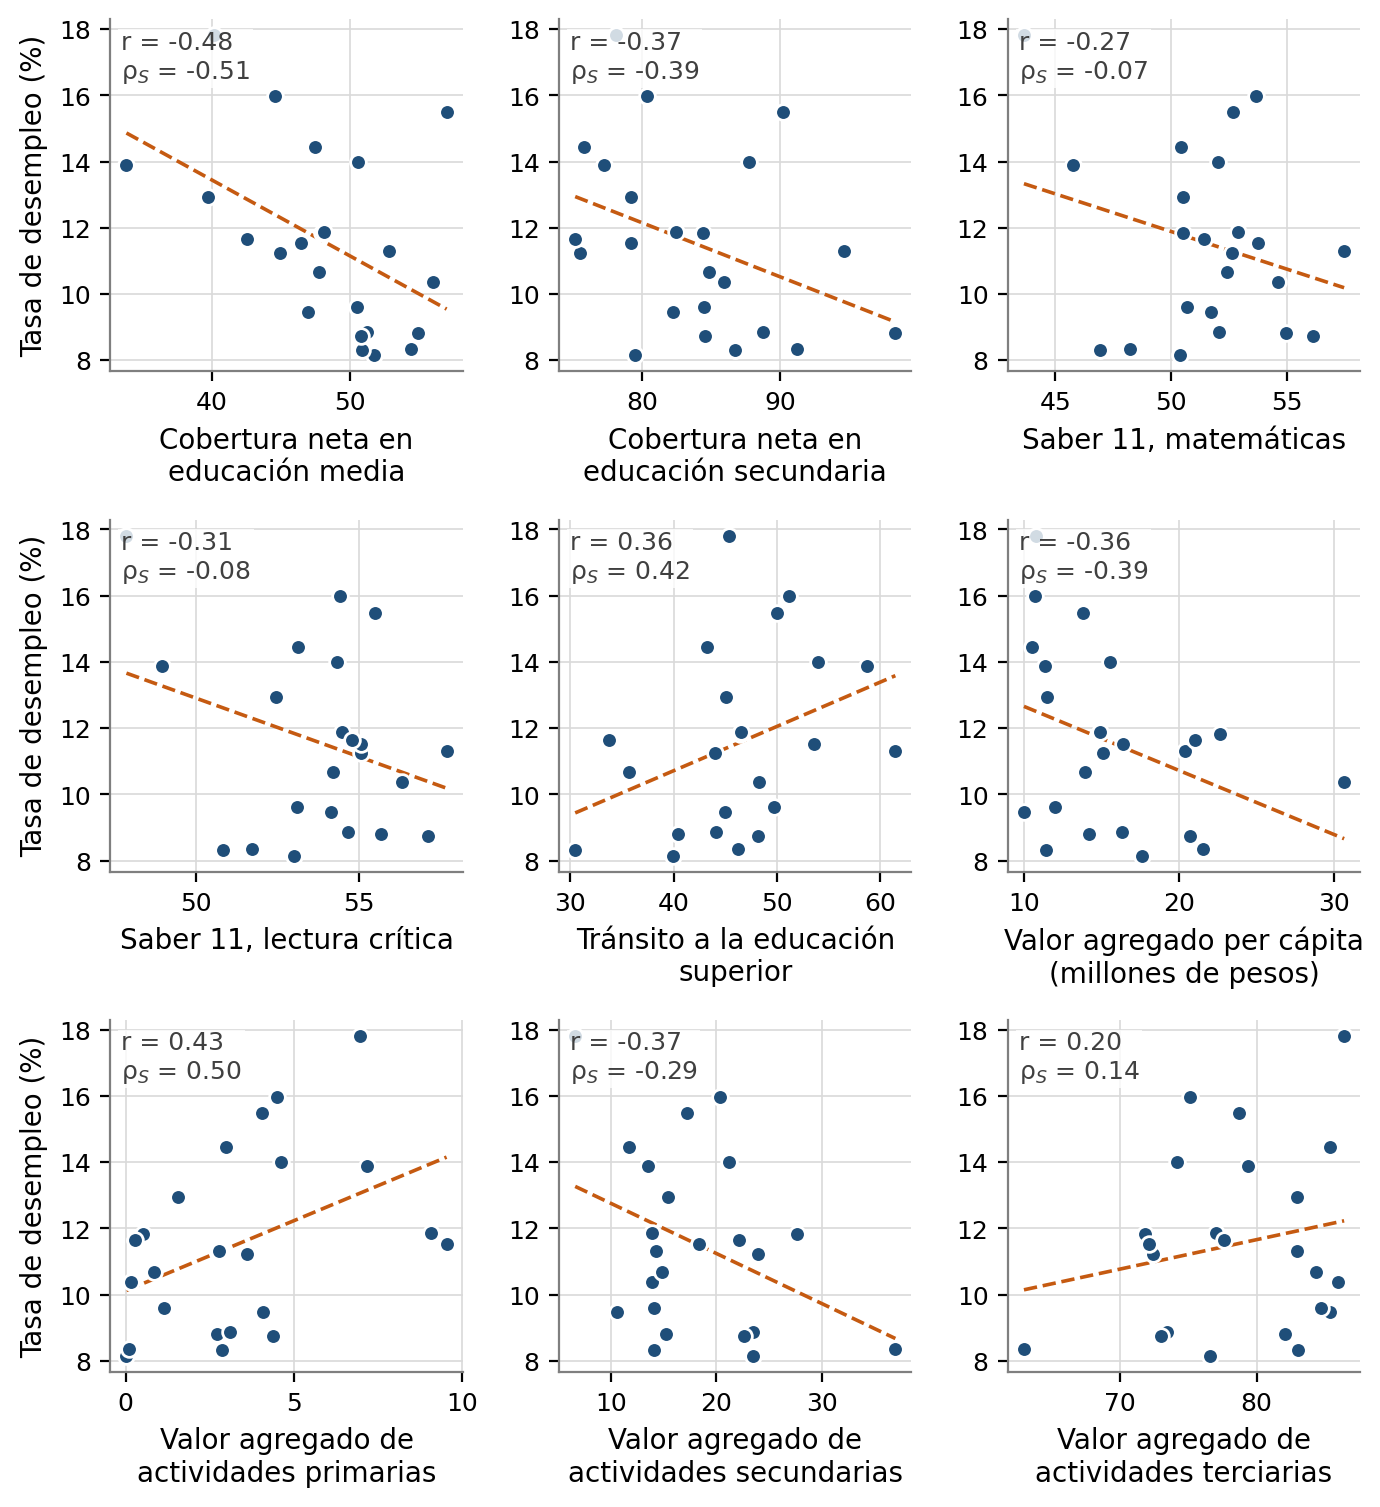
\includegraphics[width=0.9\linewidth]{img/desc_dispersion_candidatas_1.png}
\caption[Tasa directa frente a las candidatas (1 de 2)]{Tasa directa frente a las primeras nueve candidatas en los 23 dominios, con la recta de mínimos cuadrados como referencia. $r$: correlación de Pearson; $\rho_S$: correlación de Spearman. El valor agregado per cápita se expresa en millones de pesos. Fuente: tablas del análisis descriptivo.}
\label{fig:app_dispersion}
\end{figure}
\begin{figure}[!htbp]
\centering
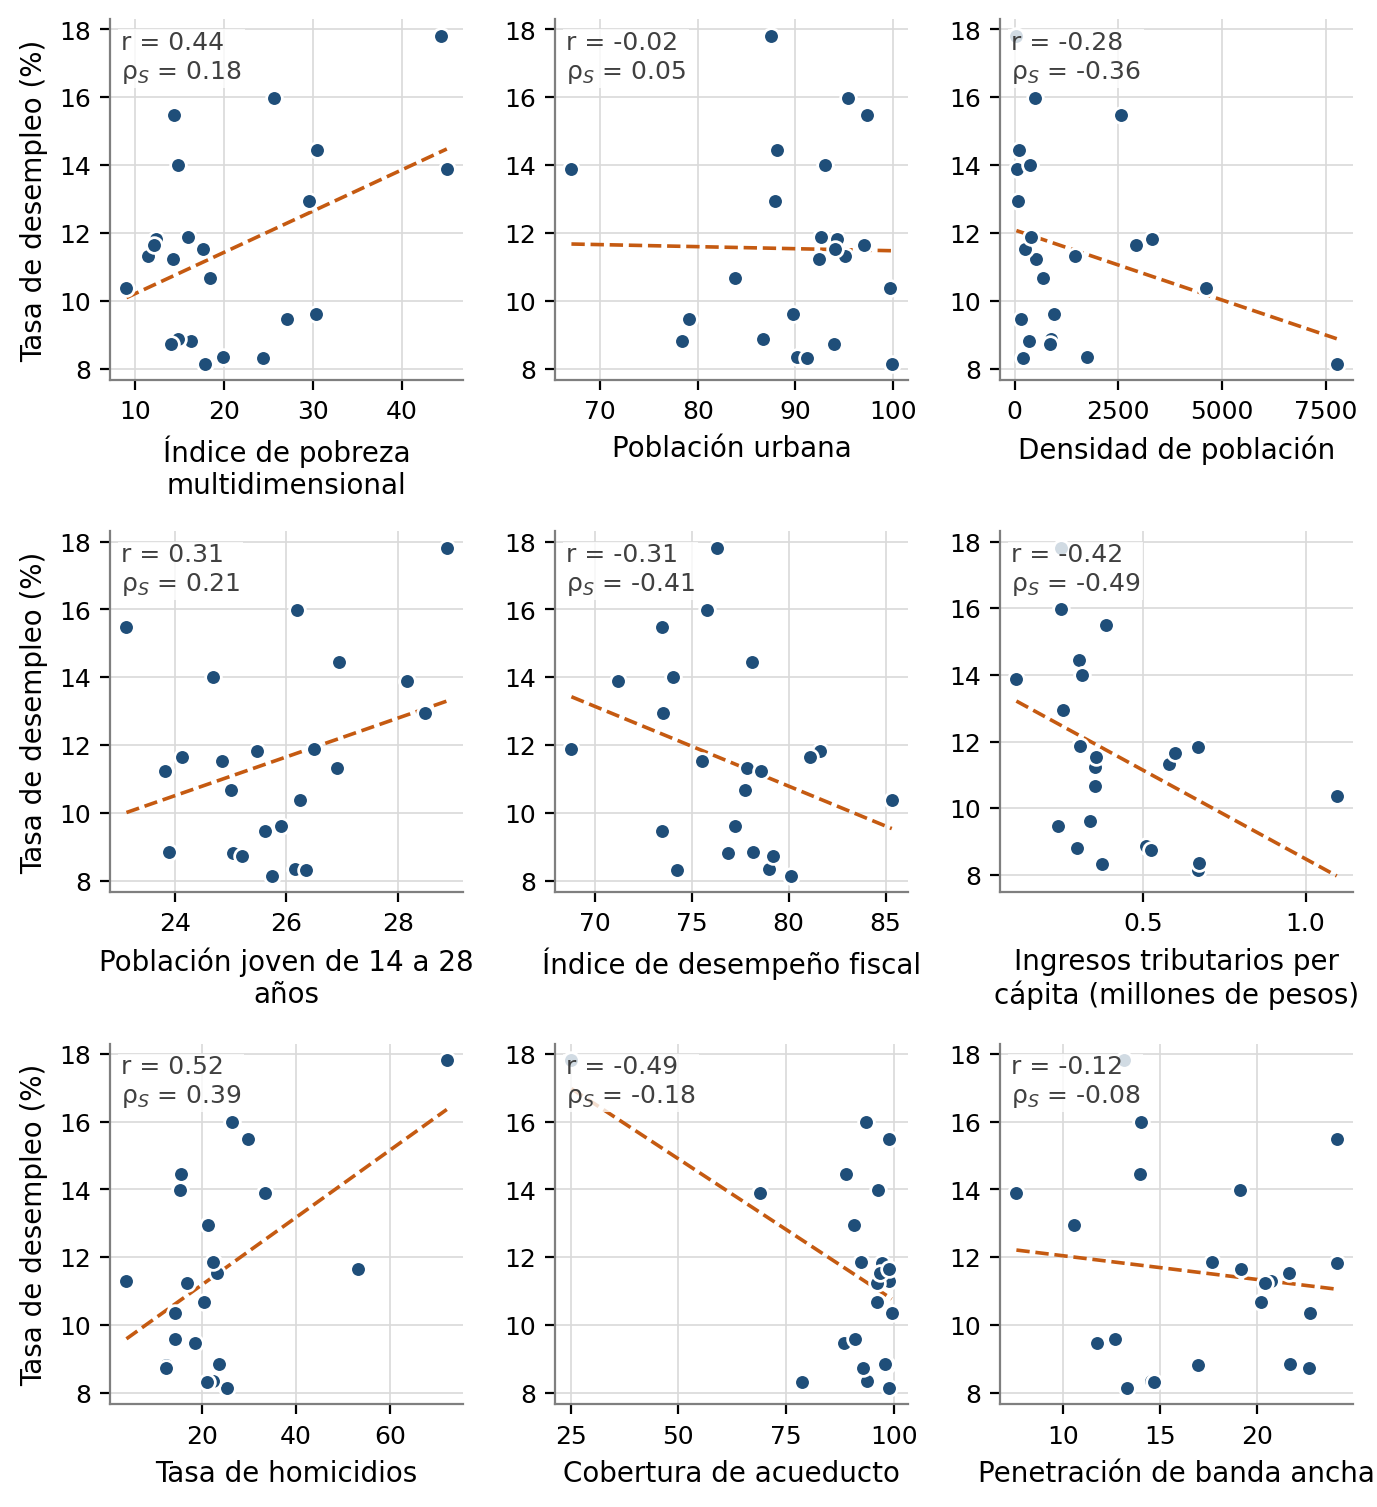
\includegraphics[width=0.9\linewidth]{img/desc_dispersion_candidatas_2.png}
\caption[Tasa directa frente a las candidatas (2 de 2)]{Tasa directa frente a las nueve candidatas restantes, con la misma lectura de la Figura~\ref{fig:app_dispersion}. Los ingresos tributarios per cápita se expresan en millones de pesos. Fuente: tablas del análisis descriptivo.}
\label{fig:app_dispersion_2}
\end{figure}
\begin{figure}[!htbp]
\centering
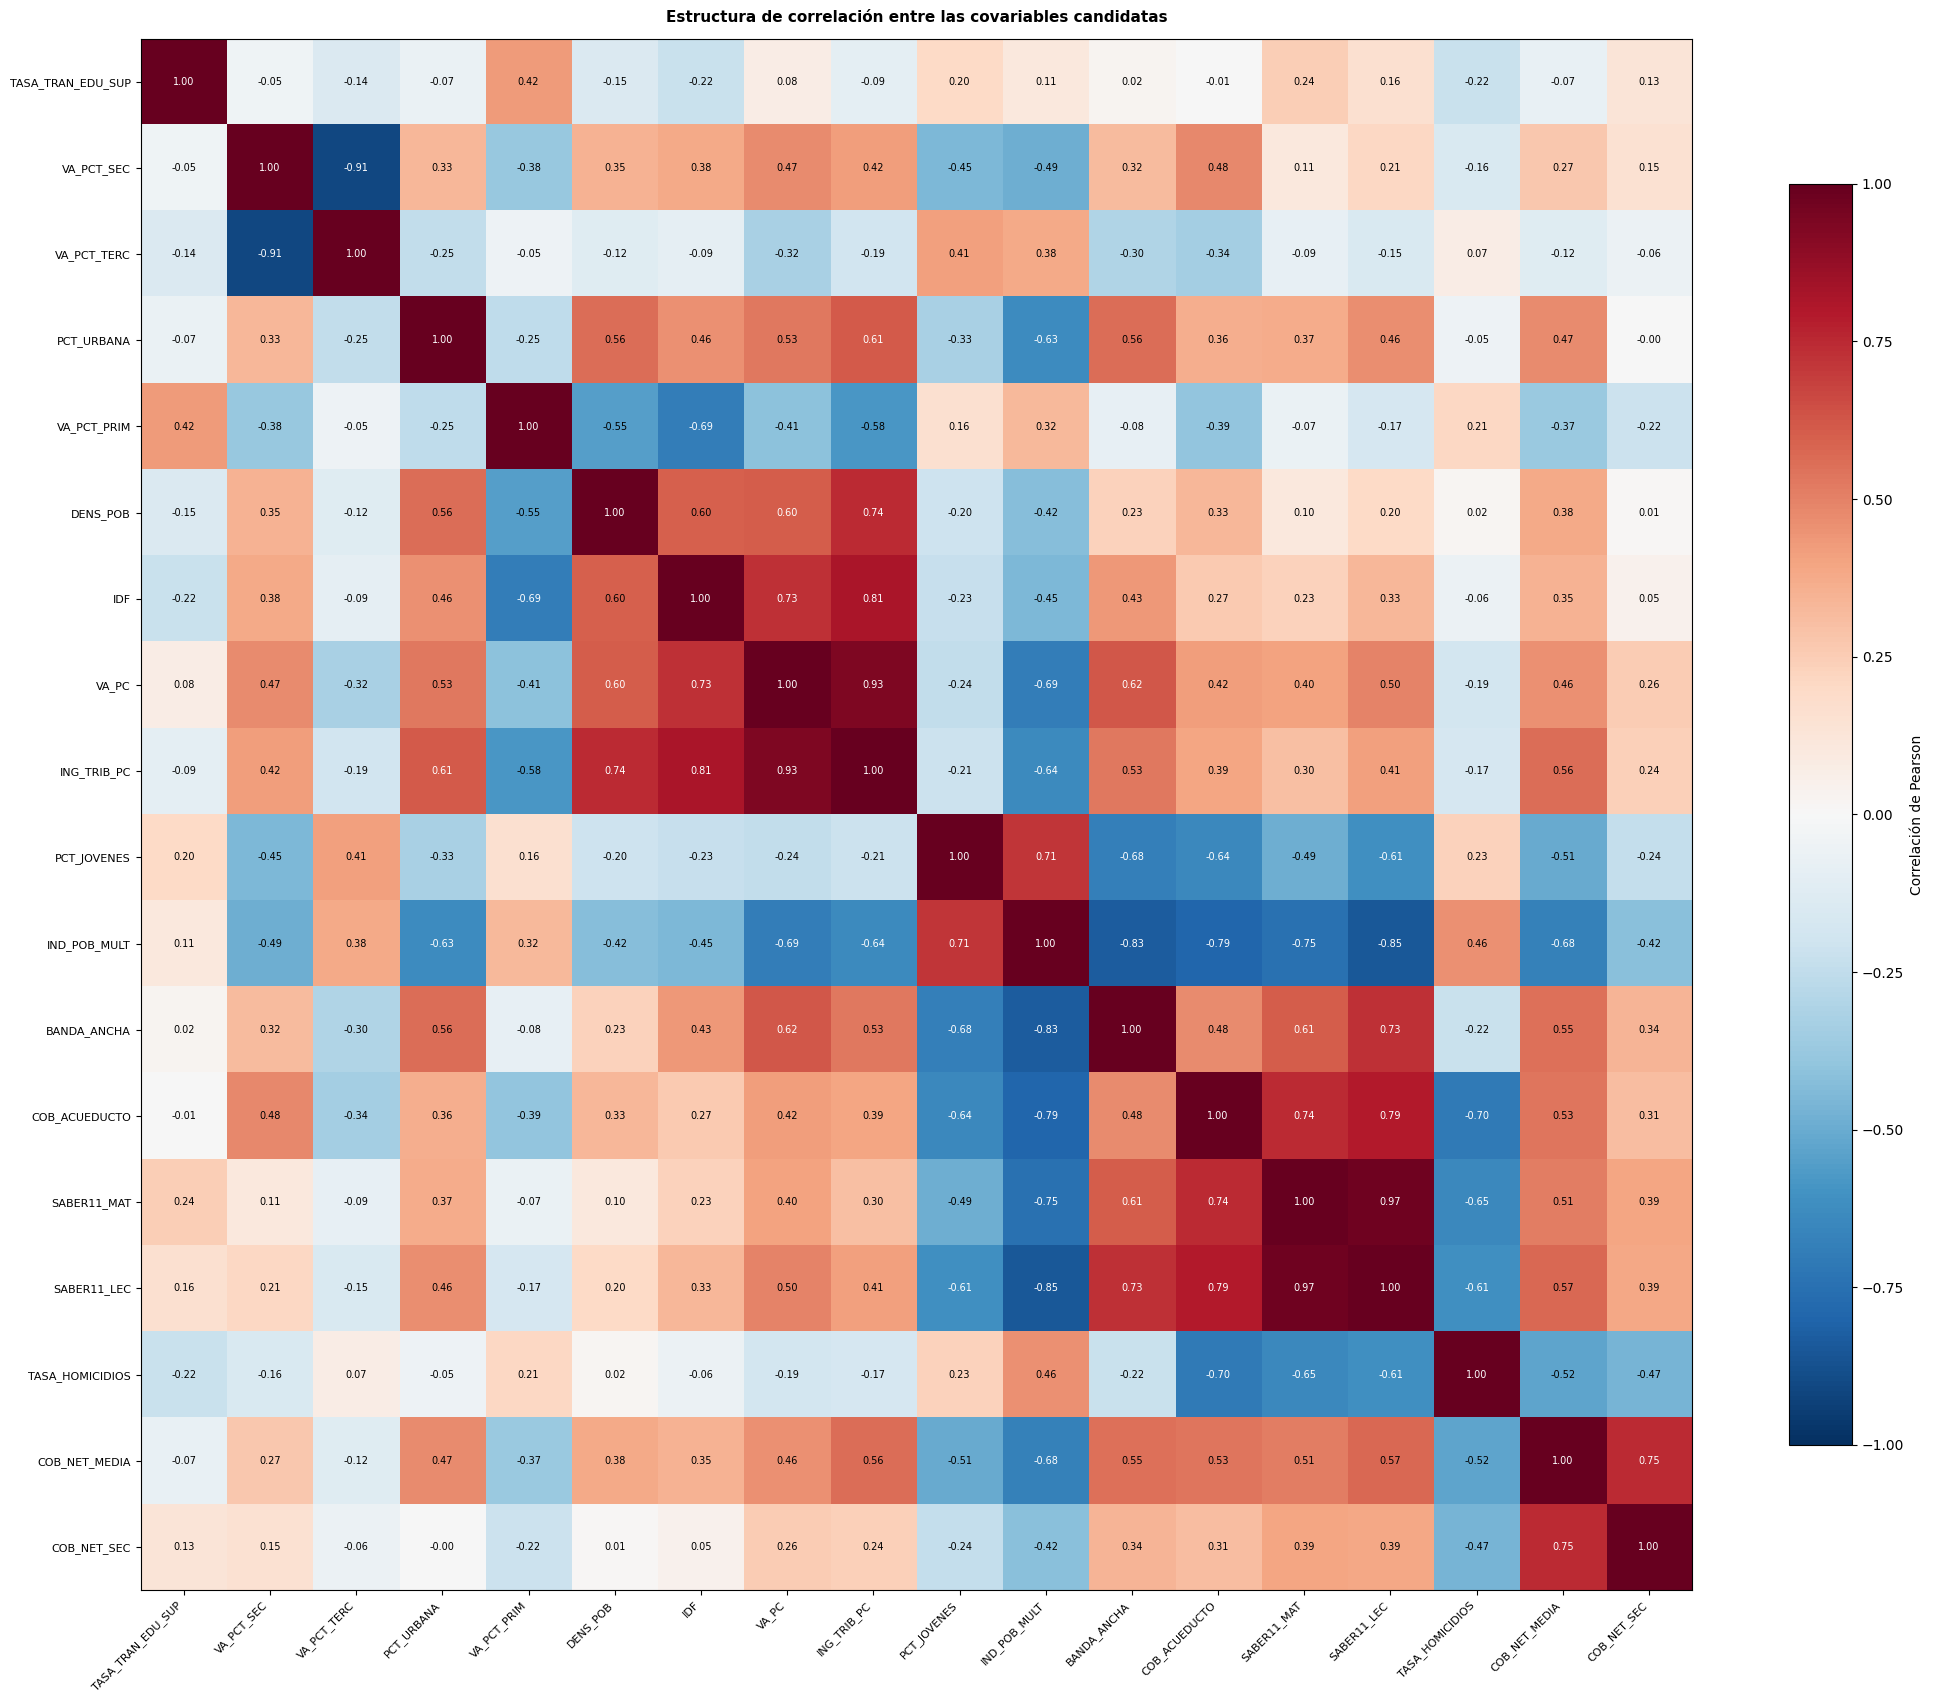
\includegraphics[width=0.9\linewidth]{img/desc_correlacion_candidatas.png}
\caption{Matriz de correlaciones de las candidatas, reordenada por agrupamiento. Fuente: tablas del análisis descriptivo.}
\label{fig:app_correlacion}
\end{figure}
%--------------------------------------------------------------------------------------
\anexo{Detalle de la selección de covariables}
\label{app:seleccion}

Esta sección presenta el Fay-Herriot univariado de cada candidata y los diagnósticos del conjunto elegido; la cita la Sección~\ref{sec:res_seleccion}.

La Tabla~\ref{tab:app_seleccion} ordena las 18 candidatas por el valor $p$ de su coeficiente. Solo tres tienen $q \le 0.10$ (tasa de homicidios, cobertura de acueducto y cobertura neta en educación media, las tres con $q = 0.079$), y Quibdó es el dominio que más mueve la correlación ponderada en ocho de las 18. Las dos covariables del conjunto elegido, tasa de homicidios y cobertura de acueducto, tienen una correlación de Pearson de $-0.70$ en los 23 dominios y un VIF de 1.984, por debajo del umbral de 5. La Figura~\ref{fig:app_residuos_parciales} muestra la relación de cada una con la tasa una vez descontado el aporte de la otra.

% D-40: la matriz de 2 por 2 (img/eda_correlacion_finales.png) se sustituyó por la frase anterior; r = -0.704 recalculado con _trabajo/calculos/datos/dominios.csv y VIF de la salida del cuaderno de selección.
{\footnotesize\setlength{\tabcolsep}{3pt}
\begin{longtable}{p{2.4cm} r p{2.3cm} r r r p{1.9cm} r}
\caption[Fay-Herriot univariado de cada candidata]{Fay-Herriot univariado de cada candidata, ajustado por REML (máxima verosimilitud restringida) y GLS (mínimos cuadrados generalizados). IC: intervalo de confianza de Wald; $q$: valor ajustado por Benjamini-Hochberg; Cook: distancia máxima; Dominio: el que más cambia $r_w$ al retirarlo; $\Delta r_w$: ese cambio; A.M.: área metropolitana. Los coeficientes están en la unidad de cada covariable, salvo el valor agregado per cápita y los ingresos tributarios per cápita (por millón de pesos) y la densidad de población (por cada 1,000 habitantes por km$^2$).}
\label{tab:app_seleccion} \\
\toprule
Covariable & $\hat{\beta}_1$ & IC 95~\% & $p$ & $q$ & Cook & Dominio & $\Delta r_w$ \\
\midrule
\endfirsthead
\multicolumn{8}{l}{\tablename~\thetable{}, continuación} \\
\toprule
Covariable & $\hat{\beta}_1$ & IC 95~\% & $p$ & $q$ & Cook & Dominio & $\Delta r_w$ \\
\midrule
\endhead
\bottomrule
\endlastfoot
Tasa de homicidios & 0.099 & [0.029, 0.170] & 0.006 & 0.079 & 0.601 & Quibdó & 0.270 \\
Cobertura de acueducto & $-0.083$ & [$-0.147$, $-0.019$] & 0.011 & 0.079 & 1.297 & Quibdó & 0.388 \\
Cobertura neta en educación media & $-0.229$ & [$-0.410$, $-0.048$] & 0.013 & 0.079 & 0.625 & Armenia & 0.177 \\
Índice de pobreza multidimensional & 0.121 & [0.015, 0.226] & 0.025 & 0.101 & 0.577 & Quibdó & 0.198 \\
Valor agregado de actividades primarias & 0.422 & [0.045, 0.798] & 0.028 & 0.101 & 0.278 & Quibdó & 0.082 \\
Ingresos tributarios per cápita & $-5.281$ & [$-10.155$, $-0.407$] & 0.034 & 0.101 & 0.845 & Bogotá & 0.069 \\
Cobertura neta en educación secundaria & $-0.163$ & [$-0.336$, 0.011] & 0.066 & 0.135 & 0.212 & Armenia & 0.109 \\
Valor agregado de actividades secundarias & $-0.150$ & [$-0.314$, 0.013] & 0.072 & 0.135 & 0.411 & Quibdó & 0.146 \\
Valor agregado per cápita & $-0.192$ & [$-0.403$, 0.019] & 0.074 & 0.135 & 0.286 & Santa Marta & 0.070 \\
Tránsito a la educación superior & 0.134 & [$-0.014$, 0.281] & 0.075 & 0.135 & 0.163 & Santa Marta & 0.080 \\
Índice de desempeño fiscal & $-0.234$ & [$-0.536$, 0.067] & 0.128 & 0.202 & 0.130 & Santa Marta & 0.058 \\
Población joven de 14 a 28 años & 0.567 & [$-0.183$, 1.318] & 0.138 & 0.202 & 0.637 & Quibdó & 0.206 \\
Saber 11, lectura crítica & $-0.352$ & [$-0.826$, 0.122] & 0.146 & 0.202 & 0.962 & Quibdó & 0.271 \\
Densidad de población & $-0.410$ & [$-1.007$, 0.186] & 0.177 & 0.228 & 0.172 & Barranquilla A.M. & 0.162 \\
Saber 11, matemáticas & $-0.224$ & [$-0.572$, 0.123] & 0.206 & 0.247 & 0.953 & Quibdó & 0.270 \\
Valor agregado de actividades terciarias & 0.088 & [$-0.098$, 0.274] & 0.353 & 0.398 & 0.315 & Cartagena & 0.130 \\
Penetración de banda ancha & $-0.069$ & [$-0.312$, 0.175] & 0.581 & 0.615 & 0.241 & Armenia & 0.125 \\
Población urbana & $-0.006$ & [$-0.159$, 0.146] & 0.938 & 0.938 & 0.524 & Riohacha & 0.166 \\
\end{longtable}
}
\begin{figure}[!htbp]
\centering
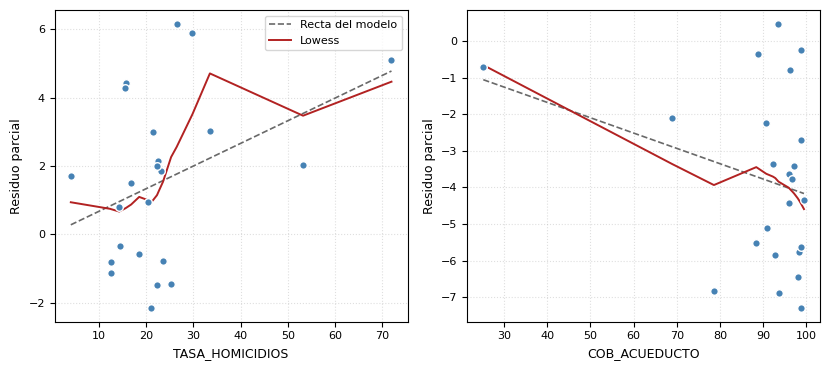
\includegraphics[width=0.9\linewidth]{img/eda_residuos_parciales.png}
\caption{Residuos parciales de las covariables seleccionadas en el Fay-Herriot con ambas. Fuente: tabla de verificación de la selección.}
\label{fig:app_residuos_parciales}
\end{figure}
%--------------------------------------------------------------------------------------
\anexo{Especificaciones del Fay-Herriot clásico}
\label{app:especificaciones}

Esta sección presenta los coeficientes y los diagnósticos de las cuatro especificaciones candidatas; la citan las Secciones~\ref{sec:res_fh_clasico} y~\ref{sec:res_supuestos}.

La Tabla~\ref{tab:app_ec_coeficientes} muestra que en EC1, con las dos covariables, ninguna tiene $p < 0.05$, mientras que en EC2 y EC3, con una covariable cada una, las dos lo cumplen. En la Tabla~\ref{tab:app_ec_diagnosticos} el valor $p$ de Shapiro-Wilk supera 0.10 en las cuatro especificaciones y EC2 tiene la mayor distancia de Cook (1.297). Las Figuras~\ref{fig:app_ec3}, \ref{fig:app_ec1}, \ref{fig:app_ec2} y~\ref{fig:app_ec0} muestran, para cada especificación, la contracción del EBLUP y la distribución de los residuos estandarizados, y la Figura~\ref{fig:app_cook} identifica los dominios que más pesan en el ajuste del benchmark.

\begin{table}[!htbp]
\centering
\small
\caption[Coeficientes de las especificaciones candidatas]{Coeficientes de las cuatro especificaciones candidatas. EE: error estándar. Fuente: salida del cuaderno del Fay-Herriot clásico.}
\label{tab:app_ec_coeficientes}
\begin{tabular}{l l r r r}
\toprule
Especificación & Parámetro & $\hat{\beta}$ & EE & $p$ \\
\midrule
EC1 & Intercepto & 13.758 & 4.997 & 0.006 \\
EC1 & Tasa de homicidios & 0.066 & 0.051 & 0.190 \\
EC1 & Cobertura de acueducto & $-0.042$ & 0.045 & 0.351 \\
EC2 & Intercepto & 19.053 & 2.994 & $<0.001$ \\
EC2 & Cobertura de acueducto & $-0.083$ & 0.033 & 0.011 \\
EC3 & Intercepto & 9.191 & 0.979 & $<0.001$ \\
EC3 & Tasa de homicidios & 0.099 & 0.036 & 0.006 \\
EC0 & Intercepto & 11.527 & 0.563 & $<0.001$ \\
\bottomrule
\end{tabular}
\end{table}
\begin{table}[!htbp]
\centering
\small
\caption[Diagnósticos de las especificaciones candidatas]{Diagnósticos de las especificaciones. DE resid.: desviación de los residuos estandarizados; SW: Shapiro-Wilk; $\psi/{\rm ECM}$: razón media entre la varianza directa y el error cuadrático medio (ECM) del EBLUP (mejor predictor lineal insesgado empírico); Influyentes: dominios con Cook $> 4/n$.}
\label{tab:app_ec_diagnosticos}
\begin{tabular}{l r r r r r r r}
\toprule
Especificación & $R^2$ & DE resid. & $p$ SW & $\bar{\gamma}$ & $\psi/{\rm ECM}$ & Cook & Influyentes \\
\midrule
EC1 & 0.299 & 0.954 & 0.391 & 0.984 & 1.011 & 0.526 & 2 \\
EC2 & 0.239 & 0.978 & 0.317 & 0.985 & 1.011 & 1.297 & 1 \\
EC3 & 0.269 & 0.977 & 0.357 & 0.984 & 1.012 & 0.601 & 2 \\
EC0 & 0.000 & 1.002 & 0.139 & 0.988 & 1.010 & 0.250 & 1 \\
\bottomrule
\end{tabular}
\end{table}
\begin{figure}[!htbp]
\centering
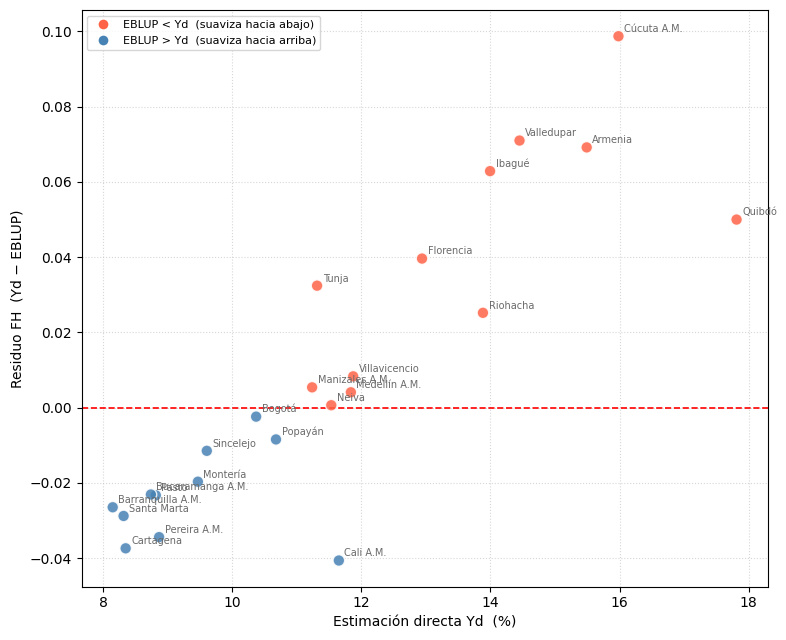
\includegraphics[width=0.48\linewidth]{img/fh_ec3_suavizador.png}
\hfill
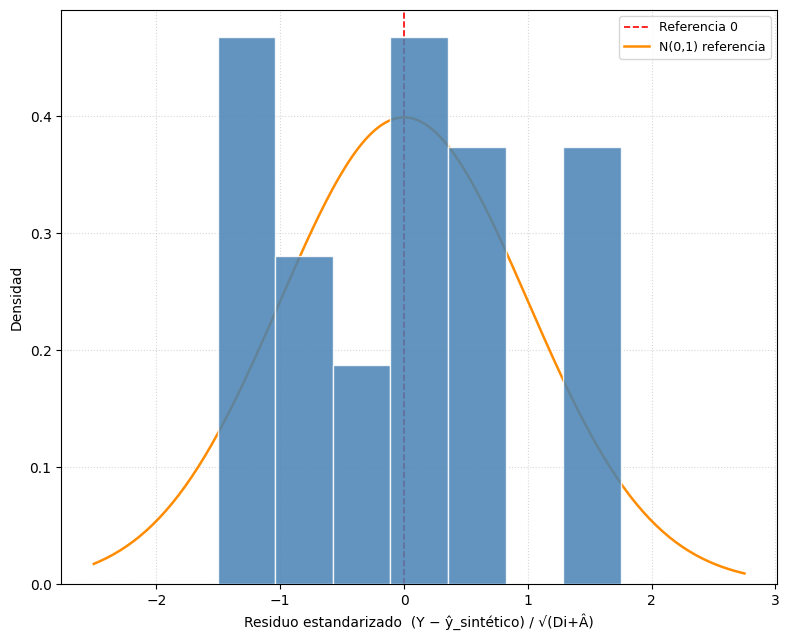
\includegraphics[width=0.48\linewidth]{img/fh_ec3_histograma.png}
\caption{Especificación EC3 (benchmark): a la izquierda, residuo del EBLUP frente a la tasa directa (contracción); a la derecha, histograma de los residuos estandarizados. Fuente: cuaderno del Fay-Herriot clásico.}
\label{fig:app_ec3}
\end{figure}
\begin{figure}[!htbp]
\centering
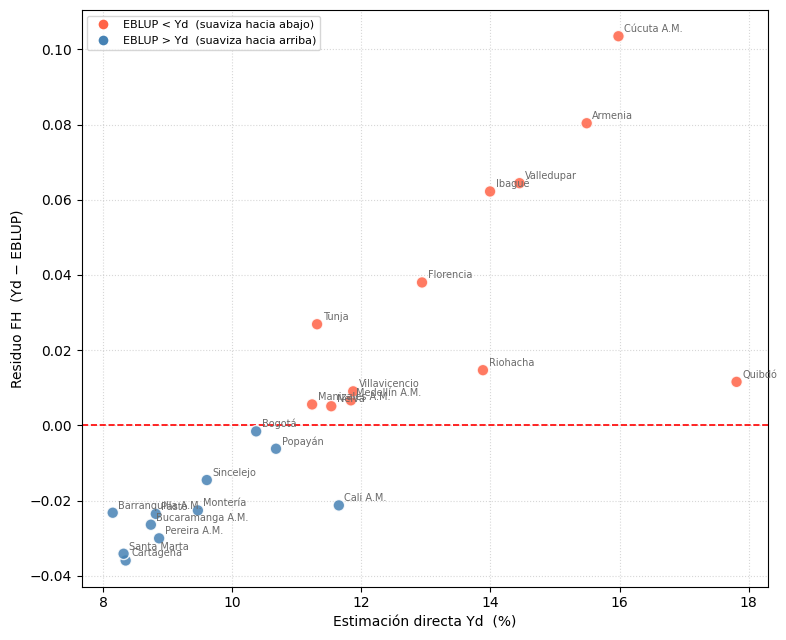
\includegraphics[width=0.48\linewidth]{img/fh_ec1_suavizador.png}
\hfill
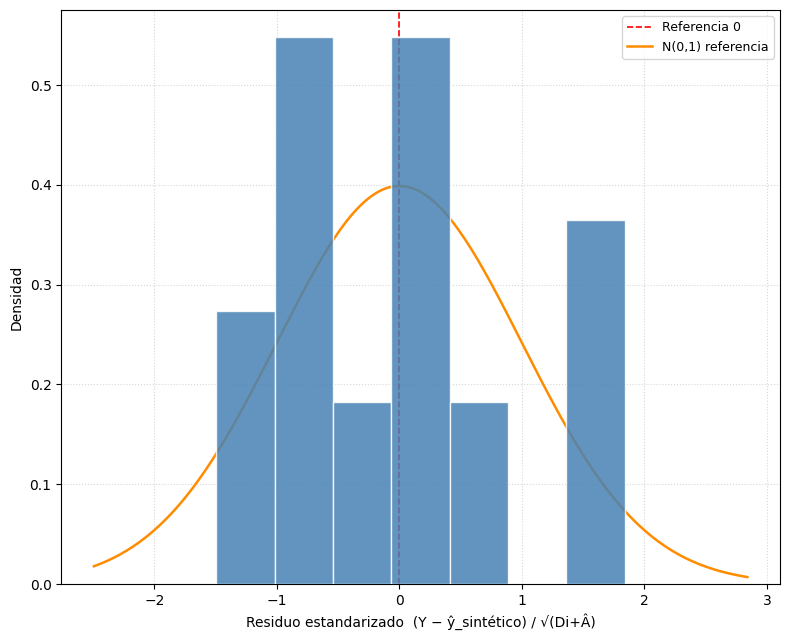
\includegraphics[width=0.48\linewidth]{img/fh_ec1_histograma.png}
\caption{Especificación EC1: a la izquierda, residuo del EBLUP frente a la tasa directa (contracción); a la derecha, histograma de los residuos estandarizados. Fuente: cuaderno del Fay-Herriot clásico.}
\label{fig:app_ec1}
\end{figure}
\begin{figure}[!htbp]
\centering
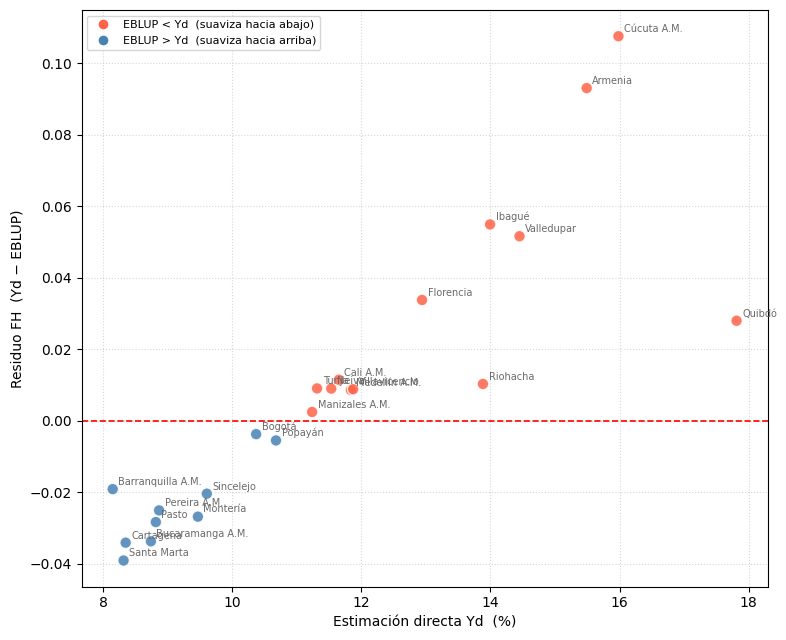
\includegraphics[width=0.48\linewidth]{img/fh_ec2_suavizador.png}
\hfill
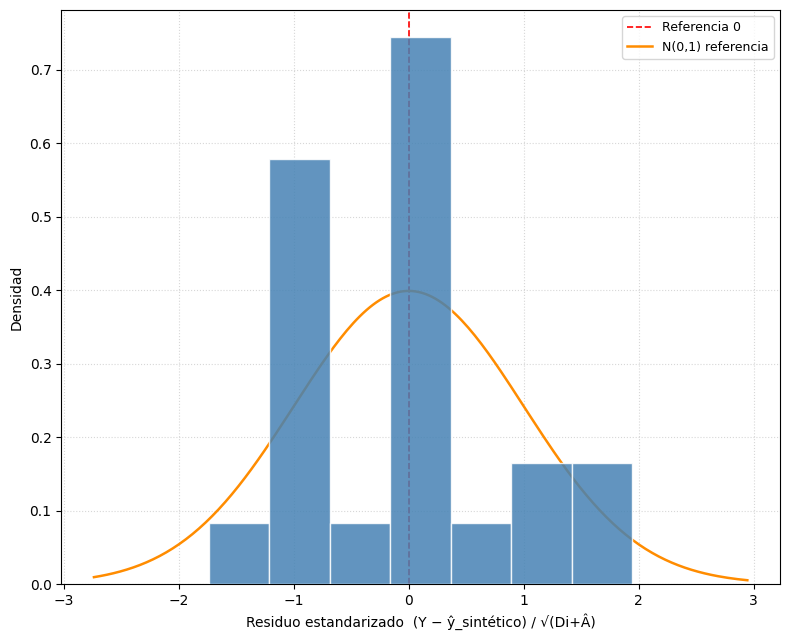
\includegraphics[width=0.48\linewidth]{img/fh_ec2_histograma.png}
\caption{Especificación EC2: a la izquierda, residuo del EBLUP frente a la tasa directa (contracción); a la derecha, histograma de los residuos estandarizados. Fuente: cuaderno del Fay-Herriot clásico.}
\label{fig:app_ec2}
\end{figure}
\begin{figure}[!htbp]
\centering
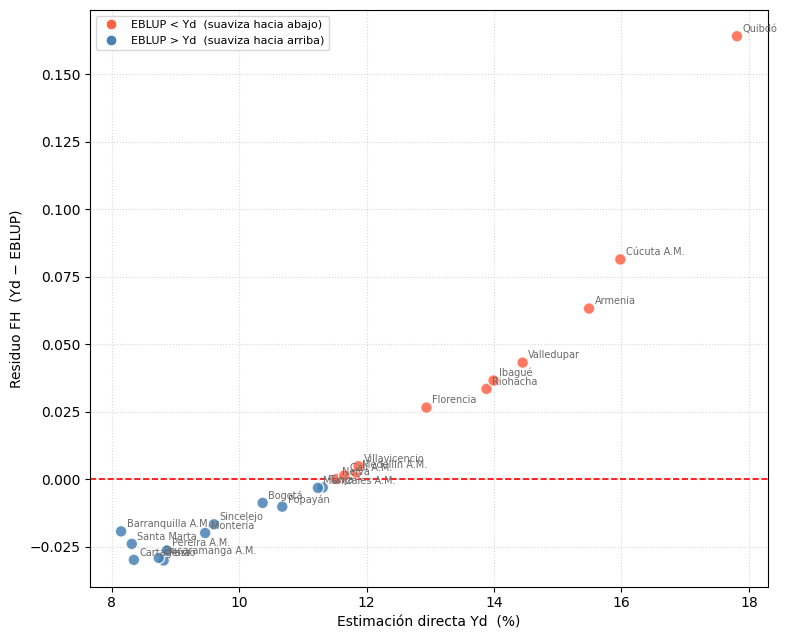
\includegraphics[width=0.48\linewidth]{img/fh_ec0_suavizador.png}
\hfill
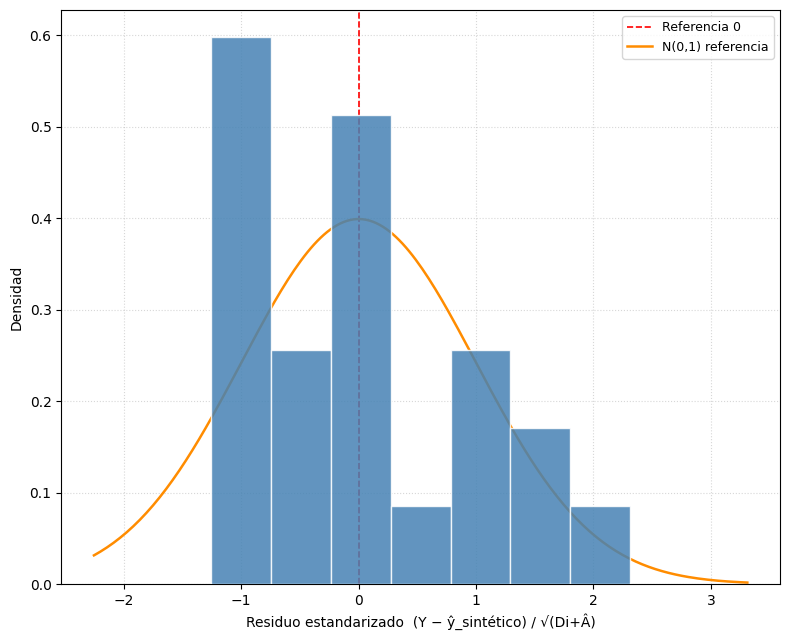
\includegraphics[width=0.48\linewidth]{img/fh_ec0_histograma.png}
\caption{Especificación EC0: a la izquierda, residuo del EBLUP frente a la tasa directa (contracción); a la derecha, histograma de los residuos estandarizados. Fuente: cuaderno del Fay-Herriot clásico.}
\label{fig:app_ec0}
\end{figure}
\begin{figure}[!htbp]
\centering
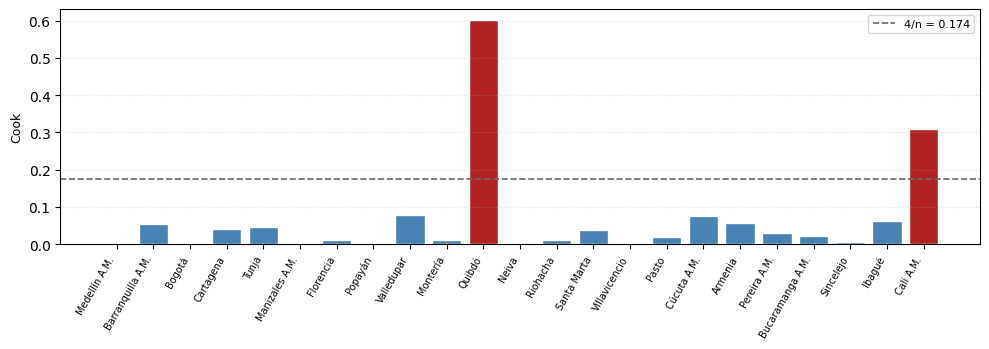
\includegraphics[width=0.85\linewidth]{img/fh_ganador_cook.png}
\caption{Distancia de Cook de cada dominio en el benchmark; la línea marca $4/n$. Fuente: tabla de Cook del Fay-Herriot clásico.}
\label{fig:app_cook}
\end{figure}
\FloatBarrier

%--------------------------------------------------------------------------------------
\anexo{Estimaciones de los dominios}
\label{app:dominios_modelo}

Esta sección presenta, para los 23 dominios, la tasa directa, el EBLUP del benchmark, el SEBLUP del escenario espacial de referencia y el EBLUP ajustado por benchmarking; la citan las Secciones~\ref{sec:res_fh_clasico} y~\ref{sec:res_espacial}.

En la Tabla~\ref{tab:app_dominios_modelo} el EBLUP y el SEBLUP se separan de la tasa directa en 0.10 puntos o menos: el peso de la directa, $\hat{\gamma}_d$, está entre 0.966 y 0.993, de modo que en los dominios los dos modelos casi reproducen la estimación directa. El benchmarking de nivel 1 mueve el EBLUP en 0.01 puntos o menos.

{\footnotesize\setlength{\tabcolsep}{3pt}
\begin{longtable}{l r r r r r r r r}
\caption[Estimaciones de los dominios]{Estimaciones de los 23 dominios, Ene-Dic 2018, en \%. CV: coeficiente de variación, en \%; EBLUP: benchmark EC3; SEBLUP: versión espacial del EBLUP, 3 vecinos, estructura completa, con error cuadrático medio por bootstrap paramétrico (tabla del SEBLUP de los dominios del cuaderno espacial); Ajustada: EBLUP tras el benchmarking de nivel 1; A.M.: área metropolitana.}
\label{tab:app_dominios_modelo} \\
\toprule
Dominio & Directa & EBLUP & CV & $\hat{\gamma}_d$ & SEBLUP & CV & $\hat{\gamma}^S_d$ & Ajustada \\
\midrule
\endfirsthead
\multicolumn{9}{l}{\tablename~\thetable{}, continuación} \\
\toprule
Dominio & Directa & EBLUP & CV & $\hat{\gamma}_d$ & SEBLUP & CV & $\hat{\gamma}^S_d$ & Ajustada \\
\midrule
\endhead
\bottomrule
\endlastfoot
Armenia & 15.49 & 15.42 & 2.20 & 0.979 & 15.43 & 2.23 & 0.978 & 15.42 \\
Barranquilla A.M. & 8.15 & 8.17 & 2.48 & 0.993 & 8.18 & 2.38 & 0.991 & 8.17 \\
Bogotá & 10.37 & 10.37 & 2.25 & 0.990 & 10.38 & 2.33 & 0.988 & 10.37 \\
Bucaramanga A.M. & 8.74 & 8.76 & 3.13 & 0.986 & 8.79 & 3.01 & 0.984 & 8.76 \\
Cali A.M. & 11.65 & 11.69 & 2.42 & 0.986 & 11.69 & 2.47 & 0.986 & 11.69 \\
Cartagena & 8.35 & 8.39 & 3.10 & 0.988 & 8.37 & 3.13 & 0.985 & 8.38 \\
Cúcuta A.M. & 15.98 & 15.88 & 2.28 & 0.976 & 15.89 & 2.33 & 0.972 & 15.88 \\
Florencia & 12.94 & 12.90 & 2.85 & 0.976 & 12.90 & 2.77 & 0.976 & 12.90 \\
Ibagué & 13.99 & 13.93 & 2.35 & 0.981 & 13.93 & 2.39 & 0.978 & 13.93 \\
Manizales A.M. & 11.24 & 11.23 & 2.52 & 0.986 & 11.23 & 2.43 & 0.984 & 11.23 \\
Medellín A.M. & 11.84 & 11.83 & 2.01 & 0.990 & 11.83 & 1.92 & 0.988 & 11.83 \\
Montería & 9.47 & 9.49 & 2.78 & 0.987 & 9.47 & 2.72 & 0.985 & 9.48 \\
Neiva & 11.53 & 11.53 & 2.67 & 0.983 & 11.53 & 2.80 & 0.983 & 11.53 \\
Pasto & 8.82 & 8.84 & 3.20 & 0.986 & 8.84 & 3.25 & 0.986 & 8.84 \\
Pereira A.M. & 8.87 & 8.90 & 3.01 & 0.987 & 8.91 & 2.98 & 0.986 & 8.90 \\
Popayán & 10.68 & 10.69 & 2.75 & 0.984 & 10.69 & 2.74 & 0.984 & 10.68 \\
Quibdó & 17.81 & 17.76 & 2.46 & 0.966 & 17.77 & 2.44 & 0.964 & 17.76 \\
Riohacha & 13.88 & 13.86 & 2.31 & 0.982 & 13.85 & 2.39 & 0.979 & 13.86 \\
Santa Marta & 8.32 & 8.35 & 2.78 & 0.990 & 8.35 & 2.88 & 0.989 & 8.34 \\
Sincelejo & 9.61 & 9.62 & 2.60 & 0.989 & 9.60 & 2.60 & 0.987 & 9.61 \\
Tunja & 11.31 & 11.28 & 2.87 & 0.981 & 11.28 & 2.83 & 0.977 & 11.28 \\
Valledupar & 14.45 & 14.38 & 2.27 & 0.981 & 14.37 & 2.29 & 0.977 & 14.38 \\
Villavicencio & 11.87 & 11.87 & 2.67 & 0.982 & 11.88 & 2.89 & 0.979 & 11.86 \\
\end{longtable}
}
%--------------------------------------------------------------------------------------
\anexo{Varianza de muestreo}
\label{app:varianza}

Esta sección presenta las varianzas alternativas de cada dominio y las figuras de la GVF y de los escenarios; la cita la Sección~\ref{sec:res_supuestos}.

La Tabla~\ref{tab:app_varianza} muestra que la varianza del bootstrap por viviendas es mayor que la del bootstrap por personas en 20 de los 23 dominios, con razones entre 0.939 y 1.173, y que la linealización de Taylor queda cerca, con razones entre 0.938 y 1.053. La Figura~\ref{fig:app_gvf} compara la varianza observada con la ajustada por las dos GVF, y la Figura~\ref{fig:app_escenarios_varianza} muestra cuánto se mueve el EBLUP de cada dominio en los ocho escenarios alternativos.

{\footnotesize\setlength{\tabcolsep}{3pt}
\begin{longtable}{l r r r r r}
\caption[Varianza de muestreo por dominio]{Varianza de muestreo por dominio: $\psi_d$ del bootstrap por viviendas (puntos porcentuales al cuadrado) y razones frente a las alternativas: bootstrap por personas, Taylor y las dos funciones generalizadas de varianza, GVF (Ecuación~\ref{eq:gvf}; razón GVF/bootstrap). A.M.: área metropolitana.}
\label{tab:app_varianza} \\
\toprule
Dominio & $\psi_d$ & Viv./pers. & Boot./Taylor & GVF A & GVF B \\
\midrule
\endfirsthead
\multicolumn{6}{l}{\tablename~\thetable{}, continuación} \\
\toprule
Dominio & $\psi_d$ & Viv./pers. & Boot./Taylor & GVF A & GVF B \\
\midrule
\endhead
\bottomrule
\endlastfoot
Armenia & 0.117 & 1.142 & 0.996 & 1.067 & 1.021 \\
Barranquilla A.M. & 0.041 & 1.026 & 1.014 & 1.028 & 1.023 \\
Bogotá & 0.055 & 1.087 & 0.974 & 1.029 & 1.044 \\
Bucaramanga A.M. & 0.076 & 1.154 & 1.041 & 0.901 & 0.876 \\
Cali A.M. & 0.081 & 1.129 & 1.032 & 0.933 & 0.931 \\
Cartagena & 0.068 & 1.005 & 1.008 & 1.010 & 0.977 \\
Cúcuta A.M. & 0.134 & 1.105 & 0.965 & 1.033 & 0.993 \\
Florencia & 0.138 & 1.155 & 1.038 & 0.896 & 0.964 \\
Ibagué & 0.108 & 1.076 & 1.006 & 1.038 & 1.028 \\
Manizales A.M. & 0.081 & 1.036 & 0.996 & 1.088 & 1.099 \\
Medellín A.M. & 0.057 & 1.141 & 1.053 & 0.921 & 0.981 \\
Montería & 0.070 & 0.997 & 0.954 & 1.036 & 1.024 \\
Neiva & 0.096 & 1.109 & 1.010 & 0.948 & 0.961 \\
Pasto & 0.081 & 1.126 & 1.034 & 0.969 & 0.969 \\
Pereira A.M. & 0.072 & 1.173 & 1.010 & 1.007 & 0.990 \\
Popayán & 0.087 & 1.082 & 0.972 & 0.980 & 0.993 \\
Quibdó & 0.193 & 1.145 & 0.995 & 0.985 & 0.975 \\
Riohacha & 0.104 & 1.065 & 0.975 & 0.999 & 0.980 \\
Santa Marta & 0.054 & 0.975 & 0.976 & 1.149 & 1.099 \\
Sincelejo & 0.063 & 1.114 & 1.016 & 1.022 & 1.007 \\
Tunja & 0.106 & 0.939 & 0.938 & 1.025 & 1.115 \\
Valledupar & 0.108 & 1.080 & 0.954 & 1.063 & 1.040 \\
Villavicencio & 0.102 & 1.104 & 1.000 & 0.953 & 0.972 \\
\end{longtable}
}
\begin{figure}[!htbp]
\centering
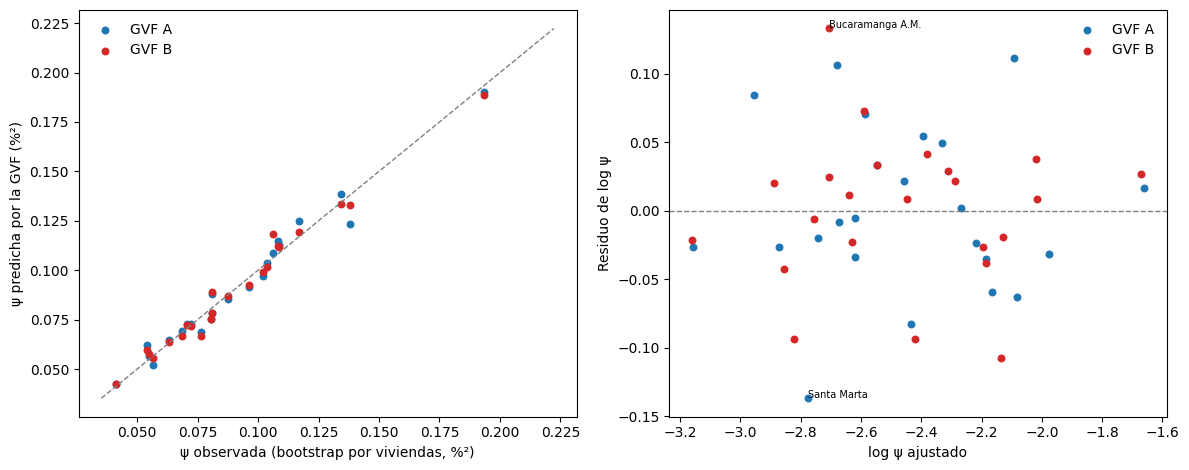
\includegraphics[width=0.9\linewidth]{img/fh_gvf_ajuste.png}
\caption{Varianza de muestreo observada frente a la ajustada por las GVF A y B. Fuente: tabla de ajuste de la GVF.}
\label{fig:app_gvf}
\end{figure}
\begin{figure}[!htbp]
\centering
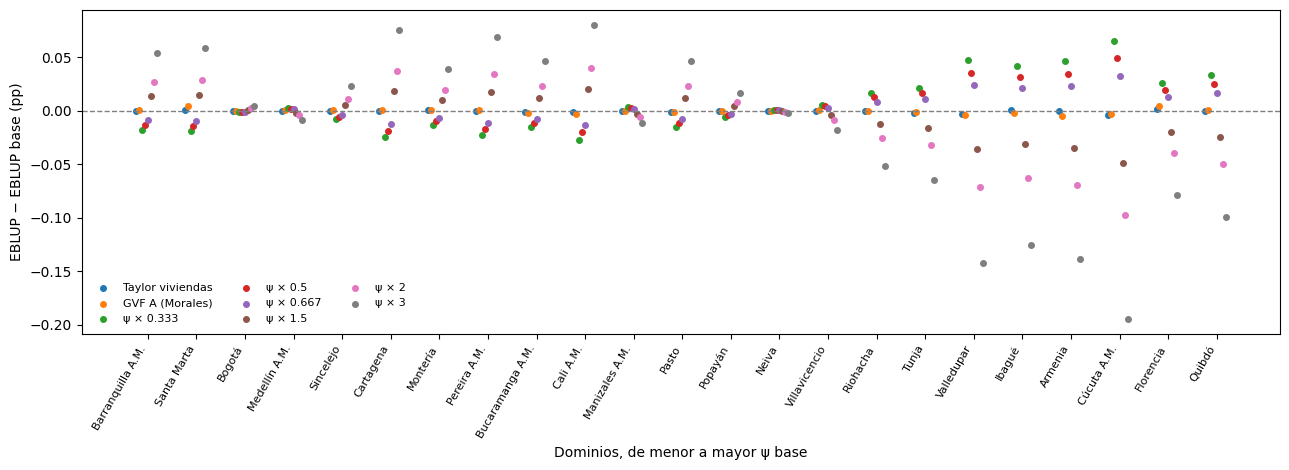
\includegraphics[width=1.0\linewidth]{img/fh_escenarios_varianza.png}
\caption{Cambio del EBLUP de cada dominio frente al escenario base en los ocho escenarios alternativos de la varianza de muestreo. Fuente: tabla de sensibilidad a la varianza por dominio.}
\label{fig:app_escenarios_varianza}
\end{figure}
%--------------------------------------------------------------------------------------
\anexo{Validación predictiva por dominio}
\label{app:validacion}

Esta sección presenta el error de cada dominio retirado en los dos ejercicios de la validación predictiva dejar-un-dominio-fuera; la cita la Sección~\ref{sec:res_validacion}.

En la Tabla~\ref{tab:app_validacion}, con el procedimiento completo el benchmark de cada iteración incluyó la tasa de homicidios en 16 de las 23 y quedó sin covariables en cuatro. Los errores más grandes aparecen cuando el conjunto cambia, como en Armenia ($-7.01$ puntos) y Quibdó ($-6.57$). La Figura~\ref{fig:app_validacion} compara la estimación del dominio retirado con su directa en los dos ejercicios.

{\footnotesize\setlength{\tabcolsep}{3pt}
\begin{longtable}{l r r r r r r r p{2.3cm}}
\caption[Validación predictiva dejar-un-dominio-fuera por dominio]{Validación predictiva dejar-un-dominio-fuera por dominio: estimación sintética del dominio retirado con las covariables fijas y con el procedimiento completo, error frente a la directa (puntos porcentuales) y error estandarizado $Z_{\text{pred}}$. A.M.: área metropolitana.}
\label{tab:app_validacion} \\
\toprule
Dominio & Directa & Fijas & Error & $Z_{\text{pred}}$ & Completo & Error & $Z_{\text{pred}}$ & Covariables (completo) \\
\midrule
\endfirsthead
\multicolumn{9}{l}{\tablename~\thetable{}, continuación} \\
\toprule
Dominio & Directa & Fijas & Error & $Z_{\text{pred}}$ & Completo & Error & $Z_{\text{pred}}$ & Covariables (completo) \\
\midrule
\endhead
\bottomrule
\endlastfoot
Armenia & 15.49 & 11.96 & $-3.53$ & $-1.49$ & 8.48 & $-7.01$ & $-3.17$ & Cobertura neta en educación media \\
Barranquilla A.M. & 8.15 & 11.87 & 3.72 & 1.60 & 11.87 & 3.72 & 1.60 & Tasa de homicidios \\
Bogotá & 10.37 & 10.63 & 0.26 & 0.10 & 5.39 & $-4.98$ & $-1.67$ & Tasa de homicidios, Ingresos tributarios per cápita \\
Bucaramanga A.M. & 8.74 & 10.57 & 1.83 & 0.74 & 10.57 & 1.83 & 0.74 & Tasa de homicidios \\
Cali A.M. & 11.65 & 15.40 & 3.75 & 1.40 & 15.40 & 3.75 & 1.40 & Tasa de homicidios \\
Cartagena & 8.35 & 11.54 & 3.20 & 1.35 & 11.54 & 3.20 & 1.35 & Tasa de homicidios \\
Cúcuta A.M. & 15.98 & 11.62 & $-4.36$ & $-1.90$ & 11.04 & $-4.94$ & $-2.15$ & Cobertura de acueducto \\
Florencia & 12.94 & 11.24 & $-1.70$ & $-0.69$ & 11.46 & $-1.48$ & $-0.52$ & ninguna \\
Ibagué & 13.99 & 10.53 & $-3.47$ & $-1.46$ & 10.53 & $-3.47$ & $-1.46$ & Tasa de homicidios \\
Manizales A.M. & 11.24 & 10.84 & $-0.40$ & $-0.16$ & 10.84 & $-0.40$ & $-0.16$ & Tasa de homicidios \\
Medellín A.M. & 11.84 & 11.42 & $-0.42$ & $-0.17$ & 11.42 & $-0.42$ & $-0.17$ & Tasa de homicidios \\
Montería & 9.47 & 11.11 & 1.64 & 0.67 & 11.11 & 1.64 & 0.67 & Tasa de homicidios \\
Neiva & 11.53 & 11.49 & $-0.04$ & $-0.02$ & 14.35 & 2.82 & 1.07 & Tasa de homicidios, Valor agregado de actividades primarias \\
Pasto & 8.82 & 10.55 & 1.74 & 0.70 & 11.65 & 2.83 & 1.03 & ninguna \\
Pereira A.M. & 8.87 & 11.65 & 2.79 & 1.16 & 11.65 & 2.79 & 1.16 & Tasa de homicidios \\
Popayán & 10.68 & 11.25 & 0.57 & 0.23 & 11.25 & 0.57 & 0.23 & Tasa de homicidios \\
Quibdó & 17.81 & 14.35 & $-3.46$ & $-0.94$ & 11.24 & $-6.57$ & $-2.66$ & ninguna \\
Riohacha & 13.88 & 12.42 & $-1.46$ & $-0.59$ & 11.42 & $-2.46$ & $-0.89$ & ninguna \\
Santa Marta & 8.32 & 11.42 & 3.10 & 1.30 & 12.82 & 4.50 & 1.91 & Cobertura de acueducto \\
Sincelejo & 9.61 & 10.69 & 1.08 & 0.43 & 10.69 & 1.08 & 0.43 & Tasa de homicidios \\
Tunja & 11.31 & 9.34 & $-1.98$ & $-0.77$ & 9.34 & $-1.98$ & $-0.77$ & Tasa de homicidios \\
Valledupar & 14.45 & 10.52 & $-3.93$ & $-1.67$ & 10.52 & $-3.93$ & $-1.67$ & Tasa de homicidios \\
Villavicencio & 11.87 & 11.39 & $-0.48$ & $-0.19$ & 11.39 & $-0.48$ & $-0.19$ & Tasa de homicidios \\
\end{longtable}
}
\begin{figure}[!htbp]
\centering
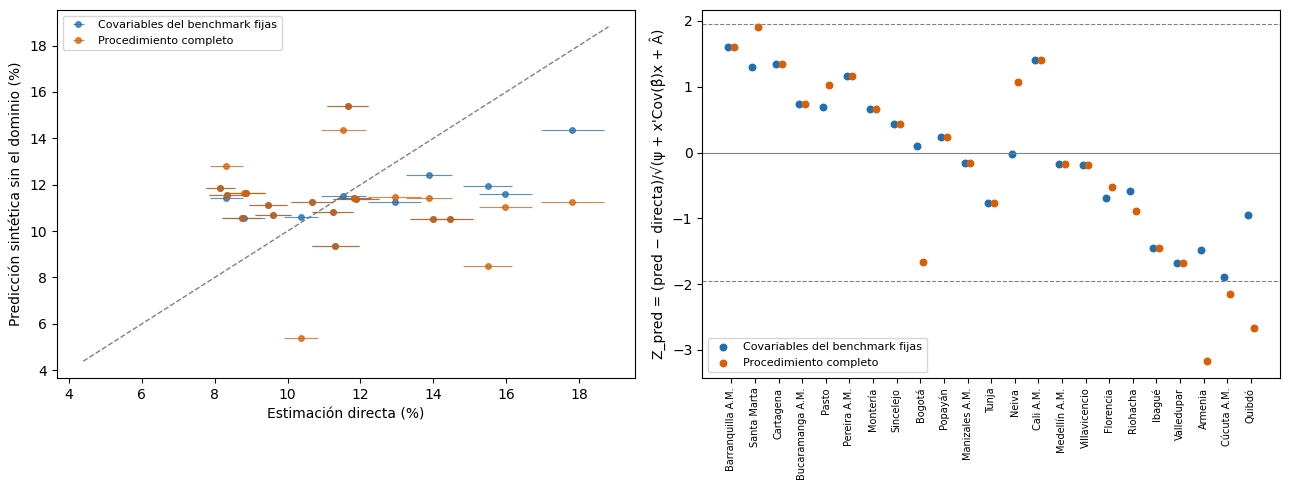
\includegraphics[width=0.9\linewidth]{img/fh_validacion_cruzada.png}
\caption{Estimación del dominio retirado frente a su estimación directa en los dos ejercicios. Fuente: tabla de validación cruzada del Fay-Herriot clásico.}
\label{fig:app_validacion}
\end{figure}
%--------------------------------------------------------------------------------------
\anexo{Detalle del modelo espacial}
\label{app:espacial}

Esta sección presenta las ocho especificaciones espaciales, su validación, sus coeficientes y las sensibilidades del parámetro $\rho$; la cita la Sección~\ref{sec:res_espacial}.

En la Tabla~\ref{tab:app_espacial} ninguna de las ocho especificaciones tiene un LRT con $p < 0.05$ (el menor es 0.221) y todas tienen un AIC mayor que el del clásico. En la validación de la Tabla~\ref{tab:app_espacial_validacion} la RMSE va de 2.35 a 2.86 puntos, frente a 2.52 del sintético clásico, y en la Tabla~\ref{tab:app_espacial_coeficientes} el coeficiente de la tasa de homicidios se mueve menos de 0.13 errores estándar entre especificaciones. Las Tablas~\ref{tab:app_espacial_rho} y~\ref{tab:app_espacial_centroide} muestran que $\hat{\rho}$ de la estructura completa depende de qué municipios entran como nodos y, en menor medida, de dónde se ubica el nodo de cada área metropolitana. Las Figuras~\ref{fig:app_perfil_rho} y~\ref{fig:app_fhe_validacion} presentan el perfil de verosimilitud de $\rho$ y la validación del escenario de referencia.

\begin{table}[!htbp]
\centering
\small
\caption[Especificaciones del Fay-Herriot espacial]{Las ocho especificaciones espaciales con la tasa de homicidios fija. AIC: criterio de información de Akaike; AIC del clásico: 108.904; $\Delta$AIC = AIC clásico $-$ AIC espacial; LRT: estadístico de la prueba de razón de verosimilitudes de $\rho = 0$.}
\label{tab:app_espacial}
\begin{adjustbox}{max width=\linewidth}
\begin{tabular}{l l r r r r r r r}
\toprule
Matriz & Estructura & $\hat{\sigma}_u^2$ & $\hat{\rho}$ & AIC & $\Delta$AIC & LRT & $p$ & $R^2$ \\
\midrule
3 vecinos & muestra & 5.383 & 0.234 & 110.572 & $-1.669$ & 0.331 & 0.565 & 0.268 \\
3 vecinos & completa & 4.825 & 0.372 & 109.403 & $-0.500$ & 1.500 & 0.221 & 0.269 \\
5 vecinos & muestra & 5.541 & 0.206 & 110.901 & $-1.998$ & 0.002 & 0.960 & 0.269 \\
5 vecinos & completa & 5.469 & 0.222 & 110.862 & $-1.958$ & 0.042 & 0.838 & 0.268 \\
Inversa, potencia 1 & muestra & 5.631 & 0.326 & 110.790 & $-1.887$ & 0.113 & 0.737 & 0.269 \\
Inversa, potencia 1 & completa & 5.479 & 0.891 & 110.894 & $-1.990$ & 0.010 & 0.922 & 0.268 \\
Inversa, potencia 2 & muestra & 5.529 & 0.187 & 110.890 & $-1.987$ & 0.013 & 0.909 & 0.269 \\
Inversa, potencia 2 & completa & 5.101 & 0.607 & 110.105 & $-1.201$ & 0.799 & 0.371 & 0.265 \\
\bottomrule
\end{tabular}
\end{adjustbox}
\end{table}
{\footnotesize\setlength{\tabcolsep}{3pt}
\begin{longtable}{p{3.2cm} l r r r r r r}
\caption[Validación del Fay-Herriot espacial por especificación]{Validación dejar-un-dominio-fuera con la tasa de homicidios fija, por especificación y estimador. RMSE: raíz del error cuadrático medio; MAE: error absoluto medio; RMSE$_c$: RMSE corregida por el ruido de muestreo. Errores en puntos porcentuales; Cob.: cobertura del intervalo del 95~\% en \%; habilidad frente al modelo de solo intercepto (RMSE 2.77).}
\label{tab:app_espacial_validacion} \\
\toprule
Especificación & Estimador & RMSE & MAE & Sesgo & RMSE$_c$ & Cob. & Habilidad \\
\midrule
\endfirsthead
\multicolumn{8}{l}{\tablename~\thetable{}, continuación} \\
\toprule
Especificación & Estimador & RMSE & MAE & Sesgo & RMSE$_c$ & Cob. & Habilidad \\
\midrule
\endhead
\bottomrule
\endlastfoot
todos & Sintético clásico & 2.52 & 2.13 & $-0.07$ & 2.51 & 100.00 & 0.17 \\
3 vecinos, muestra & Sintético espacial & 2.53 & 2.12 & $-0.02$ & 2.51 & 100.00 & 0.17 \\
3 vecinos, completa & Sintético espacial & 2.48 & 2.09 & $-0.07$ & 2.46 & 100.00 & 0.20 \\
3 vecinos, completa & Espacial con efecto & 2.35 & 1.99 & $-0.03$ & 2.33 & 100.00 & 0.28 \\
5 vecinos, muestra & Sintético espacial & 2.53 & 2.13 & $-0.10$ & 2.51 & 100.00 & 0.17 \\
5 vecinos, completa & Sintético espacial & 2.52 & 2.12 & $-0.07$ & 2.50 & 100.00 & 0.17 \\
5 vecinos, completa & Espacial con efecto & 2.59 & 2.20 & $-0.02$ & 2.57 & 100.00 & 0.13 \\
Inversa, potencia 1, muestra & Sintético espacial & 2.48 & 2.07 & $-0.25$ & 2.46 & 100.00 & 0.20 \\
Inversa, potencia 1, completa & Sintético espacial & 2.57 & 2.13 & $-0.02$ & 2.55 & 100.00 & 0.14 \\
Inversa, potencia 1, completa & Espacial con efecto & 2.60 & 2.16 & 0.02 & 2.58 & 100.00 & 0.12 \\
Inversa, potencia 2, muestra & Sintético espacial & 2.52 & 2.12 & $-0.03$ & 2.50 & 100.00 & 0.17 \\
Inversa, potencia 2, completa & Sintético espacial & 2.50 & 2.11 & 0.12 & 2.48 & 100.00 & 0.19 \\
Inversa, potencia 2, completa & Espacial con efecto & 2.86 & 2.26 & 0.24 & 2.84 & 91.30 & $-0.06$ \\
\end{longtable}
}
\begin{table}[!htbp]
\centering
\small
\caption[Coeficiente de la tasa de homicidios en el modelo espacial]{Coeficiente de la tasa de homicidios en cada especificación espacial. EE: error estándar. Clásico: 0.099 (EE 0.036, $p = 0.006$); cambio medido en errores estándar del clásico.}
\label{tab:app_espacial_coeficientes}
\begin{tabular}{l l r r r r}
\toprule
Matriz & Estructura & $\hat{\beta}_1$ & EE & $p$ & Cambio en EE \\
\midrule
3 vecinos & muestra & 0.104 & 0.035 & 0.003 & 0.118 \\
3 vecinos & completa & 0.102 & 0.035 & 0.004 & 0.069 \\
5 vecinos & muestra & 0.101 & 0.036 & 0.005 & 0.042 \\
5 vecinos & completa & 0.104 & 0.036 & 0.004 & 0.126 \\
Inversa, potencia 1 & muestra & 0.099 & 0.036 & 0.006 & 0.006 \\
Inversa, potencia 1 & completa & 0.099 & 0.036 & 0.006 & 0.000 \\
Inversa, potencia 2 & muestra & 0.100 & 0.036 & 0.005 & 0.012 \\
Inversa, potencia 2 & completa & 0.099 & 0.035 & 0.005 & $-0.021$ \\
\bottomrule
\end{tabular}
\end{table}
{\footnotesize\setlength{\tabcolsep}{3pt}
\begin{longtable}{l l r r r}
\caption[Sensibilidad de $\hat{\rho}$ a los nodos sin dato]{Sensibilidad de $\hat{\rho}$ de la estructura completa a los municipios objetivo incluidos como nodos.}
\label{tab:app_espacial_rho} \\
\toprule
Matriz & Nodos sin dato & Nodos & $\hat{\rho}$ & $p$ \\
\midrule
\endfirsthead
\multicolumn{5}{l}{\tablename~\thetable{}, continuación} \\
\toprule
Matriz & Nodos sin dato & Nodos & $\hat{\rho}$ & $p$ \\
\midrule
\endhead
\bottomrule
\endlastfoot
3 vecinos & todos & 81 & 0.372 & 0.221 \\
5 vecinos & todos & 81 & 0.222 & 0.838 \\
Inversa, potencia 1 & todos & 81 & 0.891 & 0.922 \\
Inversa, potencia 2 & todos & 81 & 0.607 & 0.371 \\
3 vecinos & solo Valle & 40 & 0.398 & 0.228 \\
5 vecinos & solo Valle & 40 & 0.273 & 0.787 \\
Inversa, potencia 1 & solo Valle & 40 & 0.990 & 0.913 \\
Inversa, potencia 2 & solo Valle & 40 & 0.690 & 0.364 \\
3 vecinos & solo Cauca & 41 & 0.262 & 0.448 \\
5 vecinos & solo Cauca & 41 & 0.157 & 0.947 \\
Inversa, potencia 1 & solo Cauca & 41 & 0.589 & 0.938 \\
Inversa, potencia 2 & solo Cauca & 41 & 0.275 & 0.735 \\
3 vecinos & ninguno & 0 & 0.234 & 0.565 \\
5 vecinos & ninguno & 0 & 0.206 & 0.960 \\
Inversa, potencia 1 & ninguno & 0 & 0.326 & 0.737 \\
Inversa, potencia 2 & ninguno & 0 & 0.187 & 0.909 \\
\end{longtable}
}
\begin{table}[!htbp]
\centering
\small
\caption[Sensibilidad a la ubicación del nodo de cada área metropolitana]{Sensibilidad a la ubicación del nodo de cada área metropolitana: en la capital o en la media de sus municipios.}
\label{tab:app_espacial_centroide}
\begin{tabular}{l l r r r r}
\toprule
Matriz & Estructura & $\hat{\rho}$ capital & $\hat{\rho}$ media & $p$ capital & $p$ media \\
\midrule
3 vecinos & muestra & 0.234 & 0.234 & 0.565 & 0.565 \\
3 vecinos & completa & 0.372 & 0.372 & 0.221 & 0.227 \\
5 vecinos & muestra & 0.206 & 0.278 & 0.960 & 0.767 \\
5 vecinos & completa & 0.222 & 0.353 & 0.838 & 0.522 \\
Inversa, potencia 1 & muestra & 0.326 & 0.403 & 0.737 & 0.788 \\
Inversa, potencia 1 & completa & 0.891 & 0.911 & 0.922 & 0.906 \\
Inversa, potencia 2 & muestra & 0.187 & 0.239 & 0.909 & 0.814 \\
Inversa, potencia 2 & completa & 0.607 & 0.616 & 0.371 & 0.354 \\
\bottomrule
\end{tabular}
\end{table}
\begin{figure}[!htbp]
\centering
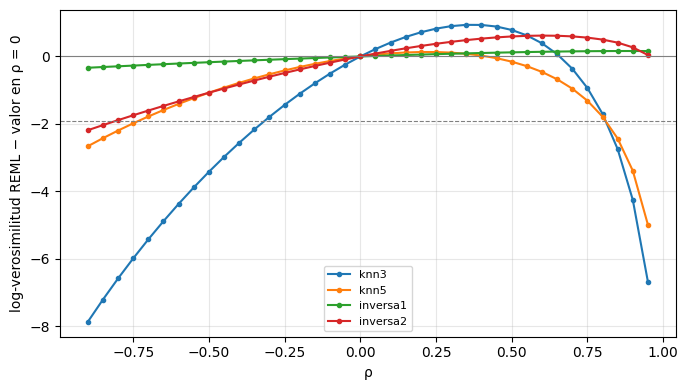
\includegraphics[width=0.85\linewidth]{img/fhe_perfil_rho.png}
\caption{Perfil de verosimilitud de $\rho$ en los cuatro escenarios de la matriz. Fuente: tabla de perfil de $\rho$.}
\label{fig:app_perfil_rho}
\end{figure}
\begin{figure}[!htbp]
\centering
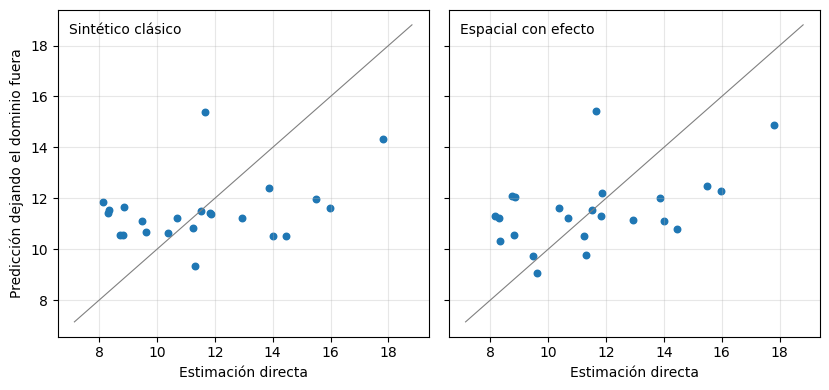
\includegraphics[width=0.9\linewidth]{img/fhe_validacion_cruzada.png}
\caption{Estimación del dominio retirado frente a la directa: sintético clásico y espacial con efecto, escenario de referencia. Fuente: tabla de validación cruzada del modelo espacial.}
\label{fig:app_fhe_validacion}
\end{figure}
\FloatBarrier

%--------------------------------------------------------------------------------------
\anexo{Estimaciones de los 83 municipios}
\label{app:municipios}

Esta sección presenta la estimación de cada municipio objetivo en la tabla final y con el modelo espacial; la citan las Secciones~\ref{sec:res_sin_muestra}, \ref{sec:res_benchmarking} y~\ref{sec:res_patrones}.

En la Tabla~\ref{tab:app_municipios} la estimación final solo difiere de la sintética en Cali y Yumbo, por el benchmarking de nivel 2, y la columna Rango marca los municipios con la tasa de homicidios fuera del rango de los dominios. Para esos municipios, la Figura~\ref{fig:app_sensibilidad_extrapolacion} muestra cuánto cambia la estimación al recortar la covariable al rango y al retirar cada dominio.

{\scriptsize\setlength{\tabcolsep}{2pt}
\begin{longtable}{l p{3.0cm} l r r r l l r r}
\caption[Estimaciones de los 83 municipios objetivo]{Estimaciones de los 83 municipios objetivo, 2018, en \%. Sin ajuste: estimación sintética del benchmark; Final: tras el benchmarking (solo cambian Cali y Yumbo); CV: coeficiente de variación, en \%; Clase: por el CV final; Rango: estado de extrapolación; Espacial: estimación espacial del escenario de referencia y su CV. Toda estimación es condicional al modelo.}
\label{tab:app_municipios} \\
\toprule
Código & Municipio & Depto. & Sin ajuste & Final & CV & Clase & Rango & Espacial & CV \\
\midrule
\endfirsthead
\multicolumn{10}{l}{\tablename~\thetable{}, continuación} \\
\toprule
Código & Municipio & Depto. & Sin ajuste & Final & CV & Clase & Rango & Espacial & CV \\
\midrule
\endhead
\bottomrule
\endlastfoot
19022 & Almaguer & Cauca & 14.57 & 14.57 & 18.15 & Aceptable & dentro & 14.59 & 18.78 \\
19050 & Argelia & Cauca & 20.96 & 20.96 & 19.93 & Aceptable & fuera & 21.17 & 20.92 \\
19075 & Balboa & Cauca & 16.71 & 16.71 & 18.25 & Aceptable & fuera & 16.75 & 18.96 \\
19100 & Bolívar & Cauca & 15.45 & 15.45 & 18.07 & Aceptable & dentro & 15.14 & 19.51 \\
19110 & Buenos Aires & Cauca & 16.77 & 16.77 & 18.27 & Aceptable & fuera & 16.87 & 18.53 \\
19130 & Cajibío & Cauca & 12.97 & 12.97 & 18.96 & Aceptable & dentro & 12.88 & 18.84 \\
19137 & Caldono & Cauca & 10.43 & 10.43 & 23.34 & No confiable & dentro & 10.39 & 23.11 \\
19142 & Caloto & Cauca & 17.74 & 17.74 & 18.56 & Aceptable & fuera & 17.84 & 18.86 \\
19212 & Corinto & Cauca & 31.17 & 31.17 & 24.09 & No confiable & fuera & 31.60 & 24.63 \\
19256 & El Tambo & Cauca & 17.66 & 17.66 & 18.53 & Aceptable & fuera & 17.69 & 18.28 \\
19290 & Florencia & Cauca & 13.01 & 13.01 & 18.93 & Aceptable & dentro & 12.59 & 19.61 \\
19300 & Guachené & Cauca & 18.27 & 18.27 & 18.76 & Aceptable & fuera & 18.32 & 18.09 \\
19318 & Guapi & Cauca & 10.99 & 10.99 & 21.94 & No confiable & dentro & 10.95 & 22.37 \\
19355 & Inzá & Cauca & 9.88 & 9.88 & 25.06 & No confiable & dentro & 10.14 & 24.77 \\
19364 & Jambaló & Cauca & 10.86 & 10.86 & 22.23 & No confiable & dentro & 10.84 & 21.05 \\
19392 & La Sierra & Cauca & 11.96 & 11.96 & 20.13 & No confiable & dentro & 11.95 & 20.79 \\
19397 & La Vega & Cauca & 10.41 & 10.41 & 23.42 & No confiable & dentro & 10.40 & 23.93 \\
19418 & López & Cauca & 15.07 & 15.07 & 18.08 & Aceptable & dentro & 15.12 & 17.49 \\
19450 & Mercaderes & Cauca & 16.19 & 16.19 & 18.14 & Aceptable & dentro & 15.85 & 19.08 \\
19455 & Miranda & Cauca & 15.84 & 15.84 & 18.10 & Aceptable & dentro & 15.88 & 18.28 \\
19473 & Morales & Cauca & 11.49 & 11.49 & 20.91 & No confiable & dentro & 11.45 & 20.55 \\
19513 & Padilla & Cauca & 12.19 & 12.19 & 19.81 & Aceptable & dentro & 12.07 & 20.58 \\
19532 & Patía & Cauca & 20.50 & 20.50 & 19.72 & Aceptable & fuera & 20.70 & 20.37 \\
19533 & Piamonte & Cauca & 11.44 & 11.44 & 21.00 & No confiable & dentro & 11.88 & 20.54 \\
19548 & Piendamó & Cauca & 11.14 & 11.14 & 21.61 & No confiable & dentro & 11.10 & 22.07 \\
19573 & Puerto Tejada & Cauca & 24.46 & 24.46 & 21.52 & No confiable & fuera & 24.08 & 20.78 \\
19585 & Puracé & Cauca & 9.19 & 9.19 & 27.71 & No confiable & fuera & 9.01 & 28.06 \\
19517 & Paéz & Cauca & 10.71 & 10.71 & 22.61 & No confiable & dentro & 10.73 & 22.96 \\
19622 & Rosas & Cauca & 12.65 & 12.65 & 19.26 & Aceptable & dentro & 12.63 & 20.83 \\
19693 & San Sebastián & Cauca & 10.10 & 10.10 & 24.34 & No confiable & dentro & 10.10 & 24.32 \\
19701 & Santa Rosa & Cauca & 11.05 & 11.05 & 21.80 & No confiable & dentro & 11.39 & 20.81 \\
19698 & Santander de Quilichao & Cauca & 15.21 & 15.21 & 18.07 & Aceptable & dentro & 15.27 & 18.65 \\
19743 & Silvia & Cauca & 9.19 & 9.19 & 27.71 & No confiable & fuera & 9.16 & 28.64 \\
19760 & Sotará & Cauca & 11.33 & 11.33 & 21.22 & No confiable & dentro & 11.27 & 22.10 \\
19785 & Sucre & Cauca & 11.28 & 11.28 & 21.31 & No confiable & dentro & 11.26 & 21.42 \\
19780 & Suárez & Cauca & 16.66 & 16.66 & 18.24 & Aceptable & fuera & 16.76 & 18.34 \\
19809 & Timbiquí & Cauca & 14.52 & 14.52 & 18.16 & Aceptable & dentro & 14.57 & 18.55 \\
19807 & Timbío & Cauca & 11.43 & 11.43 & 21.03 & No confiable & dentro & 11.30 & 21.29 \\
19821 & Toribío & Cauca & 10.60 & 10.60 & 22.89 & No confiable & dentro & 10.55 & 23.14 \\
19824 & Totoró & Cauca & 11.21 & 11.21 & 21.45 & No confiable & dentro & 11.22 & 20.97 \\
19845 & Villa Rica & Cauca & 17.34 & 17.34 & 18.43 & Aceptable & fuera & 17.24 & 17.88 \\
76020 & Alcalá & Valle & 13.43 & 13.43 & 18.62 & Aceptable & dentro & 14.01 & 16.46 \\
76036 & Andalucía & Valle & 17.60 & 17.60 & 18.51 & Aceptable & fuera & 17.73 & 19.13 \\
76041 & Ansermanuevo & Valle & 20.00 & 20.00 & 19.49 & Aceptable & fuera & 20.22 & 18.36 \\
76054 & Argelia & Valle & 20.23 & 20.23 & 19.59 & Aceptable & fuera & 20.71 & 18.50 \\
76100 & Bolívar & Valle & 16.01 & 16.01 & 18.12 & Aceptable & dentro & 16.12 & 18.10 \\
76109 & Buenaventura & Valle & 12.12 & 12.12 & 19.90 & Aceptable & dentro & 12.12 & 20.66 \\
76113 & Bugalagrande & Valle & 15.72 & 15.72 & 18.09 & Aceptable & dentro & 15.82 & 18.88 \\
76122 & Caicedonia & Valle & 15.73 & 15.73 & 18.09 & Aceptable & dentro & 16.53 & 17.34 \\
76126 & Calima & Valle & 11.94 & 11.94 & 20.16 & No confiable & dentro & 11.93 & 20.11 \\
76130 & Candelaria & Valle & 15.57 & 15.57 & 18.08 & Aceptable & dentro & 15.02 & 17.23 \\
76147 & Cartago & Valle & 12.55 & 12.55 & 19.37 & Aceptable & dentro & 12.20 & 19.87 \\
76233 & Dagua & Valle & 11.85 & 11.85 & 20.29 & No confiable & dentro & 11.84 & 19.67 \\
76246 & El Cairo & Valle & 10.64 & 10.64 & 22.78 & No confiable & dentro & 10.89 & 22.31 \\
76248 & El Cerrito & Valle & 16.05 & 16.05 & 18.12 & Aceptable & dentro & 16.12 & 18.43 \\
76250 & El Dovio & Valle & 13.66 & 13.66 & 18.48 & Aceptable & dentro & 13.70 & 18.74 \\
76243 & El Águila & Valle & 27.02 & 27.02 & 22.59 & No confiable & fuera & 27.65 & 21.54 \\
76275 & Florida & Valle & 12.30 & 12.30 & 19.66 & Aceptable & dentro & 12.18 & 19.74 \\
76306 & Ginebra & Valle & 9.19 & 9.19 & 27.71 & No confiable & fuera & 9.11 & 28.02 \\
76318 & Guacarí & Valle & 19.36 & 19.36 & 19.21 & Aceptable & fuera & 19.53 & 19.31 \\
76111 & Guadalajara de Buga & Valle & 14.72 & 14.72 & 18.12 & Aceptable & dentro & 14.78 & 18.23 \\
76364 & Jamundí & Valle & 15.65 & 15.65 & 18.08 & Aceptable & dentro & 14.91 & 17.15 \\
76377 & La Cumbre & Valle & 11.02 & 11.02 & 21.87 & No confiable & dentro & 10.98 & 22.12 \\
76400 & La Unión & Valle & 14.75 & 14.75 & 18.11 & Aceptable & dentro & 14.82 & 18.13 \\
76403 & La Victoria & Valle & 15.71 & 15.71 & 18.08 & Aceptable & dentro & 15.81 & 18.35 \\
76497 & Obando & Valle & 14.83 & 14.83 & 18.10 & Aceptable & dentro & 14.86 & 18.04 \\
76520 & Palmira & Valle & 13.62 & 13.62 & 18.50 & Aceptable & dentro & 13.52 & 18.98 \\
76563 & Pradera & Valle & 15.03 & 15.03 & 18.08 & Aceptable & dentro & 14.95 & 17.62 \\
76606 & Restrepo & Valle & 11.78 & 11.78 & 20.40 & No confiable & dentro & 11.77 & 20.69 \\
76616 & Riofrío & Valle & 11.74 & 11.74 & 20.47 & No confiable & dentro & 11.73 & 22.30 \\
76622 & Roldanillo & Valle & 11.62 & 11.62 & 20.68 & No confiable & dentro & 11.62 & 21.01 \\
76670 & San Pedro & Valle & 13.29 & 13.29 & 18.71 & Aceptable & dentro & 13.32 & 19.78 \\
76001 & Cali & Valle & 14.36 & 11.60 & 29.96 & No confiable & dentro & 11.57 & 21.35 \\
76736 & Sevilla & Valle & 11.55 & 11.55 & 20.81 & No confiable & dentro & 11.67 & 21.16 \\
76823 & Toro & Valle & 18.70 & 18.70 & 18.93 & Aceptable & fuera & 18.92 & 18.88 \\
76828 & Trujillo & Valle & 11.26 & 11.26 & 21.36 & No confiable & dentro & 11.23 & 23.10 \\
76834 & Tuluá & Valle & 13.90 & 13.90 & 18.36 & Aceptable & dentro & 13.95 & 17.82 \\
76845 & Ulloa & Valle & 12.82 & 12.82 & 19.09 & Aceptable & dentro & 13.49 & 17.13 \\
76863 & Versalles & Valle & 11.92 & 11.92 & 20.19 & No confiable & dentro & 11.96 & 21.43 \\
76869 & Vijes & Valle & 9.97 & 9.97 & 24.75 & No confiable & dentro & 9.91 & 24.38 \\
76890 & Yotoco & Valle & 11.05 & 11.05 & 21.80 & No confiable & dentro & 11.02 & 22.15 \\
76892 & Yumbo & Valle & 16.96 & 13.70 & 30.03 & No confiable & fuera & 14.24 & 20.72 \\
76895 & Zarzal & Valle & 14.40 & 14.40 & 18.19 & Aceptable & dentro & 14.56 & 17.83 \\
\end{longtable}
}
\begin{figure}[!htbp]
\centering
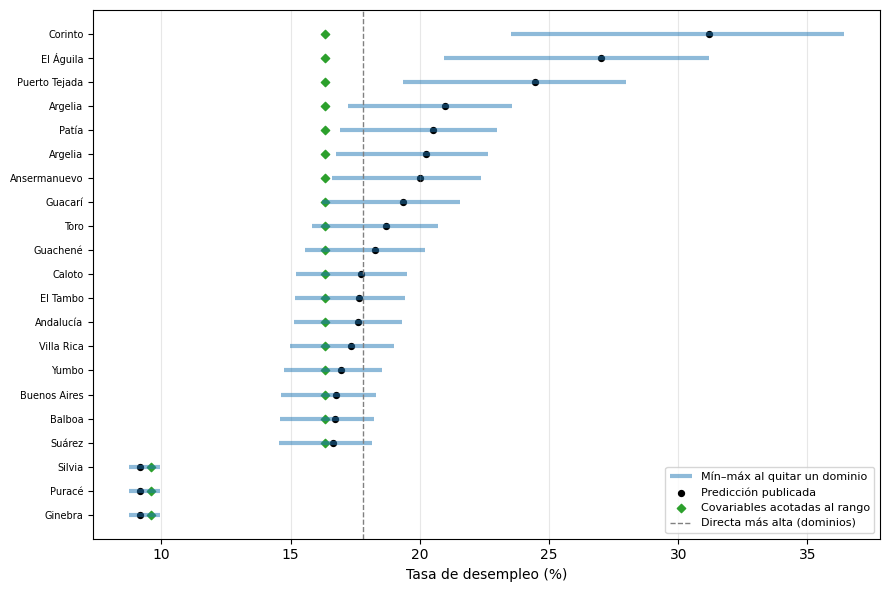
\includegraphics[width=0.9\linewidth]{img/fh_sensibilidad_extrapolacion.png}
\caption{Municipios que extrapolan: estimación publicada, estimación con la tasa de homicidios recortada al rango de los dominios y franja de la estimación al retirar cada dominio. Fuente: tabla de sensibilidad de la extrapolación.}
\label{fig:app_sensibilidad_extrapolacion}
\end{figure}
%--------------------------------------------------------------------------------------
\anexo{Material complementario de Resultados}
\label{app:resultados}

Esta sección reúne tablas de apoyo de la Sección~\ref{sec:resultados} que no responden por sí solas a un objetivo; cada una se cita desde la sección de Resultados que complementa.

\subsection{Tratamiento de faltantes y atípicos}

Complementa la Sección~\ref{sec:res_faltantes}.

\begin{table}[!htbp]
\centering
\small
\caption{Resultado del tratamiento de faltantes y atípicos.}
\label{tab:res_faltantes}
\begin{tabularx}{\linewidth}{>{\raggedright\arraybackslash}p{4.6cm} >{\raggedright\arraybackslash}X}
\toprule
Caso & Resultado \\
\midrule
Factor de expansión faltante & 0 personas; el procesamiento no se detuvo \\
Registros sin código de área & \num{152314} personas de 2018 (762,753 menos 610,439 con área) no se usan; 9 capitales no tienen registros con código de área en 2018 \\
Indicadores de TerriData con faltantes en los dominios & \num{1073} de \num{1582}; salen en el pre-filtrado \\
Candidatas con faltantes en los municipios objetivo & 0 de 18 \\
Valores atípicos en las candidatas (regla del diagrama de caja) & 22 casos en 13 de las 18; Quibdó y Riohacha son los dominios que más se repiten; ninguno se eliminó \\
Valores atípicos en la tasa directa & Ninguno \\
\bottomrule
\end{tabularx}
\end{table}

\subsection{Variables de la literatura sin dato utilizable}

Complementa la Sección~\ref{sec:res_covariables}.

\begin{table}[!htbp]
\centering
\small
\caption{Variables de la revisión de literatura sin dato utilizable.}
\label{tab:res_excluidas}
\begin{tabularx}{\linewidth}{>{\raggedright\arraybackslash}p{5.2cm} >{\raggedright\arraybackslash}X}
\toprule
Variable & Motivo \\
\midrule
Tasa de analfabetismo (censo) & Sin dato en los dominios con encuesta para 2018 \\
Empresas generadoras de empleo formal por cada 10,000 habitantes & La serie termina en 2016 \\
Incidencia de la pobreza monetaria & Solo departamentos y 23 ciudades; no existe en los municipios objetivo \\
Coeficiente de Gini & Solo departamental \\
Víctimas de desplazamiento forzado ubicadas & Solo 2022 y 2023 \\
Índice de incidencia del conflicto armado & Retirado: mide el conflicto en el propio municipio; $r = 0.92$ con la tasa de homicidios en los dominios; 13 valores distintos \\
\bottomrule
\end{tabularx}
\end{table}

\subsection{Sensibilidad de las covariables de las áreas metropolitanas a la regla de agregación}

Complementa la Sección~\ref{sec:res_covariables}.

\begin{table}[!htbp]
\centering
\small
\caption[Sensibilidad de las covariables de las áreas metropolitanas a la regla de agregación]{Cambio relativo máximo en los 7 dominios con área metropolitana (A.M.) entre la agregación con el denominador propio y la agregación con la población de 15 años y más. Solo se muestran las variables con cambio de 1~\% o más; en las otras 14 es menor.}
\label{tab:res_agregacion_am}
\begin{adjustbox}{max width=\linewidth}
\begin{tabular}{l l r l}
\toprule
Covariable & Denominador propio & Cambio máximo (\%) & Dominio \\
\midrule
Densidad de población & Superficie & 67.67 & Bucaramanga A.M. \\
Valor agregado de actividades secundarias & Valor agregado & 43.94 & Cali A.M. \\
Valor agregado de actividades primarias & Valor agregado & 14.23 & Manizales A.M. \\
Valor agregado de actividades terciarias & Valor agregado & 8.04 & Cali A.M. \\
\bottomrule
\end{tabular}
\end{adjustbox}
\end{table}

\subsection{Frecuencia de selección en la validación con el procedimiento completo}

Complementa la Sección~\ref{sec:res_validacion}.

\begin{table}[!htbp]
\centering
\small
\caption{Frecuencia con que cada covariable entra en las 23 iteraciones del procedimiento completo, en la selección de covariables y en el benchmark.}
\label{tab:res_frecuencia}
\begin{tabular}{l r r}
\toprule
Covariable & Selección (\%) & Benchmark (\%) \\
\midrule
Tasa de homicidios & 78.26 & 69.57 \\
Cobertura de acueducto & 56.52 & 8.70 \\
Cobertura neta en educación media & 8.70 & 4.35 \\
Ingresos tributarios per cápita & 4.35 & 4.35 \\
Valor agregado de actividades primarias & 4.35 & 4.35 \\
Ninguna (solo intercepto) & 17.39 & 17.39 \\
\bottomrule
\end{tabular}
\end{table}

\subsection{Validación dejar-un-dominio-fuera del modelo espacial}

Complementa la Sección~\ref{sec:res_espacial}.

\begin{table}[!htbp]
\centering
\small
\caption[Validación del escenario espacial de referencia]{Validación predictiva dejar-un-dominio-fuera con la tasa de homicidios fija, escenario de referencia (3 vecinos, estructura completa). RMSE: raíz del error cuadrático medio; MAE: error absoluto medio. Errores en puntos porcentuales. Las métricas de los cuatro escenarios están en el Apéndice~\ref{app:espacial}.}
\label{tab:res_validacion_espacial}
\begin{adjustbox}{max width=\linewidth}
\begin{tabular}{l r r r r r}
\toprule
Estimador del dominio retirado & RMSE & MAE & Sesgo & Cobertura (\%) & Habilidad \\
\midrule
Sintético clásico & 2.52 & 2.13 & $-0.07$ & 100.00 & 0.17 \\
Sintético espacial & 2.48 & 2.09 & $-0.07$ & 100.00 & 0.20 \\
Espacial con efecto & 2.35 & 1.99 & $-0.03$ & 100.00 & 0.28 \\
Solo intercepto & 2.77 & 2.23 & $-0.01$ & 95.65 & no aplica \\
\bottomrule
\end{tabular}
\end{adjustbox}
\end{table}

\FloatBarrier


    \end{appendices}
\end{document}